%% ----------------------------------------------------------------
%% Thesis.tex -- MAIN FILE (the one that you compile with LaTeX)
%% ---------------------------------------------------------------- 

% Set up the document
\documentclass[a4paper, 11pt, oneside]{Thesis}  % Use the "Thesis" style, based on the ECS Thesis style by Steve Gunn
\graphicspath{Figures/}  % Location of the graphics files (set up for graphics to be in PDF format)

% Include any extra LaTeX packages required
\usepackage[square, numbers, comma, sort&compress]{natbib}  % Use the "Natbib" style for the references in the Bibliography
\usepackage{verbatim}  % Needed for the "comment" environment to make LaTeX comments
\usepackage{vector}  % Allows "\bvec{}" and "\buvec{}" for "blackboard" style bold vectors in maths
\hypersetup{urlcolor=blue, colorlinks=true}  % Colours hyperlinks in blue, but this can be distracting if there are many links.
\makeglossaries
%% ----------------------------------------------------------------
\begin{document}
\frontmatter      % Begin Roman style (i, ii, iii, iv...) page numbering

% Set up the Title Page
\title  {Reverse Engineering Object-Oriented Systems into Umple: An Incremental and Rule-Based Approach}
\authors  {\texorpdfstring
            {\href{mgarzon@uottawa.ca}{Miguel A. Garz\'{o}n Torres}}
            {Miguel A. Garz\'{o}n}
            }
\date  {\normalsize \copyright  Miguel Garz\'{o}n, Ottawa, Canada, 2015}

\maketitle
%% ----------------------------------------------------------------

\setstretch{1.3}  % It is better to have smaller font and larger line spacing than the other way round

% Define the page headers using the FancyHdr package and set up for one-sided printing
\fancyhead{}  % Clears all page headers and footers

\rhead{\thepage}  % Sets the right side header to show the page number
\lhead{}  % Clears the left side page header

\pagestyle{fancy}  % Finally, use the "fancy" page style to implement the FancyHdr headers

%% ----------------------------------------------------------------
% The "Funny Quote Page"
\pagestyle{empty}  % No headers or footers for the following pages
\null\vfill
% Now comes the "Funny Quote", written in italics
\textit{``Live as if you were to die tomorrow. Learn as if you were to live forever.''}

\begin{flushright}
Mahatma Gandhi   
\end{flushright}

\vfill\vfill\vfill\vfill\vfill\vfill\null
\clearpage  % Funny Quote page ended, start a new page
%% ----------------------------------------------------------------

% The Abstract Page
\addtotoc{Abstract}  % Add the "Abstract" page entry to the Contents
\abstract{
\addtocontents{toc}{\vspace{1em}}  % Add a gap in the Contents, for aesthetics

This thesis investigates a novel approach to reverse engineering, in which modeling information such as UML associations, state machines and attributes is incrementally added to code written in Java or C++, while maintaining the system in a textual format. Umple is a textual representation that blends modeling in UML with programming language code. The approach, called umplification, produces a program with behavior identical to the original one, but written in Umple and enhanced with model-level abstractions. As the resulting program is Umple code, our approach eliminates the distinction between code and model. We implemented automated umplification in  a tool called the Umplificator. The tool is rule-driven: code, including Umple code, is parsed and processed into an internal representation, which is then operated on by rules; transformed textual code and model, in Umple, is then generated. The rules used to transform code to model have been iteratively refined by using the tool on a variety of open-source software systems.

The thesis consists of three main parts. The first part (Chapters 1 and 2) present the research questions and research methodology, as well as introducing Umple and the background necessary to understand the rest of the thesis. The umplification method is presented at increasing levels of detail through Chapters 3 and 4. Chapters 5 and 6 present the tool and evaluation of our approach, respectively. An analysis of related work, and comparison to our own, appears in Chapter 7.
}

\clearpage  % Abstract ended, start a new page
%% ----------------------------------------------------------------

\setstretch{1.3}  % Reset the line-spacing to 1.3 for body text (if it has changed)

% The Acknowledgements page, for thanking everyone
\acknowledgements{
\addtocontents{toc}{\vspace{1em}}  % Add a gap in the Contents, for aesthetics

Foremost, I would like to express my sincere gratitude to my dear supervisor, Professor Timothy Lethbridge, for guiding me during my graduate studies. I greatly appreciate his vast knowledge, dedication and assistance in writing proposals, scholarship applications, papers and this thesis. Throughout my studies, Tim contributed to my development as a researcher, professor and as a person.

Besides my supervisor, I would also like to thank the members of my PhD committee for the feedback provided at the different stages or this research. 

My sincere thanks to Professors Daniel Amyot and Liam Peyton for the continuous encouragement to my work. More than my instructors, they have been mentors who helped shape my career path. 

I thank each of the members of the Complexity Reduction in Software Engineering (CRuiSE) research group. Particular and well deserved thanks to Hamoud Aljamaan for all of his constructive feedback.

I wish to deeply thank the University of Ottawa for being my second home for the past 10 years and for offering me all the support required to carry out my research work.

I would also like to thank my whole family for the support they provided me through my entire life. In particular, I would like to thank my mother Patricia, my brothers Laura and Sebastian for their love and encouragement during this busy period of my life.

Last, but not least, I would like to thank my wife Idalia for her understanding and love during the past few years and for her contribution on the graphics of this thesis.
}
\clearpage  % End of the Acknowledgements
%% ----------------------------------------------------------------

\pagestyle{fancy}  %The page style headers have been "empty" all this time, now use the "fancy" headers as defined before to bring them back


%% ----------------------------------------------------------------
\lhead{\emph{Contents}}  % Set the left side page header to "Contents"
\tableofcontents  % Write out the Table of Contents

%% ----------------------------------------------------------------
\lhead{\emph{List of Figures}}  % Set the left side page header to "List if Figures"
\listoffigures  % Write out the List of Figures

%% ----------------------------------------------------------------
\lhead{\emph{List of Tables}}  % Set the left side page header to "List of Tables"
\listoftables  % Write out the List of Tables

%% ----------------------------------------------------------------
%\lhead{\emph{List of Listings}}  
%\lstlistoflistings  % Write out the List of Tables
%% ----------------------------------------------------------------
\setstretch{1.5}  % Set the line spacing to 1.5, this makes the following tables easier to read
\clearpage  % Start a new page
\lhead{\emph{Glossary}}  % Set the left side page header to "Abbreviations"
%% ----------------------------------------------------------------
\mainmatter	  % Begin normal, numeric (1,2,3...) page numbering
\pagestyle{fancy}  % Return the page headers back to the "fancy" style

% Include the chapters of the thesis, as separate files
% Just uncomment the lines as you write the chapters
\lhead{\emph{\rightmark}} 

\chapter{Introduction}

In this thesis, we present the design and analysis of a reverse-engineering technique called Umplification. Our approach makes it possible to incrementally refactor existing programs so that textual Umple abstractions come to be incorporated into the code. Such programs can be maintained using visual UML(Unified Modeling Language) modeling tools or text editors.  Umplification hence eliminates the distinction between modeling and programming since the end-product of umplification is not a separate model, but is an incremental change to the code/model. 

Many software systems experience growth and change for an extended period of time. Maintaining consistency between documentation and the corresponding code becomes challenging. This situation has long been recognized by researchers, and significant effort has been made to tackle it. Reverse engineering is one of the fruits of this effort and has been defined as the process of creating a representation of the system at a higher level of abstraction \cite{Chikofsky}.

Reverse engineering, in general, recovers documentation from code of software systems. When such documentation follows a well-defined syntax, it is often now referred to as a model.  Such models are often represented using UML, which visually represents the static and dynamic characteristics of a system. 

There is a long and rich literature in reverse engineering \cite{CanforaHarman2007}. Most existing techniques result in the generation of documentation that can be consulted separately from the code. Other techniques generate models in the form of UML diagrams that are intended to be used for code generation of a new version of the system. The technique discussed in this thesis goes one step further: It modifies the source code to add model constructs that are represented textually, but can also be viewed and edited as diagrams. The target language of our reverse engineering process is Umple \cite{UmpleMAIN}, which adds UML and other constructs textually to Java, C++ and PHP.
%FINAL CHANGE START
\textit{Umplification} comes from the play on words with the concept of `amplification' and also the notion of converting into Umple. Earlier work from our research group \cite{Lethbridge2010c} found that umplifying code is reasonably straightforward for someone familiar with Umple, and with knowledge of UML modeling pragmatics. Moreover, manual umplification of several systems, including the Umple compiler itself, has been performed by other members of our research group.
%FINAL CHANGE END
The present thesis focuses on how the umplification process can be performed automatically using reverse engineering technology. This thesis presents an automated approach for detection and transformation of Umple constructs.

In the next section, we state the research problem addressed by this thesis and list the research questions. Then, we present the methodology that we will follow in order to answer our research questions.

\section{Problem Statement}
The problem to be addressed in this research is as follows:

Developers currently often work with large volumes of legacy code. Tools exist to allow them to extract models or transform their code in a variety of ways. However doing so tends to result in a system that is quite different in syntax and structure. They are thus inhibited from using reverse engineering tools except to generate documentation.

%TLFINAL split paragraph here
The Umple technology partially solves this problem by allowing incremental addition of modeling constructs into familiar programming language code. This allows developers to maintain the essential `familiarity' with their code as they gradually transform it. Converting to Umple (Umplification) has been done manually; indeed, it was applied to the Umple compiler itself \cite{Lethbridge2010c} –  but it ought to have tool support so it can be done in a more automatic, systematic and error-free manner on large systems. We present an approach that automatically extracts the model from an object-oriented system in the form of Umple code. 

\section{Research Questions}

The guiding research questions that have motivated our research are the following:
%FINAL CHANGE START
\paragraph*{RQ1. To what extent can we achieve automated umplification?}
Although, in previous work, other members of our research group have found that the process of extracting an Umple model from source code can be relatively easily performed if done manually; our investigation focuses on performing the process automatically by means of a reverse engineering technology. 
In this thesis, we address this research question by exploring technology alternatives, developing and refining a tool, and then evaluating and assessing the effectiveness of the products of the tool. The latter is described in Chapter \ref{chap:evaluation}.
%FINAL CHANGE END
%Notice the rewrite above. You do not give answers in this part of the thesis. Leave that to the conclusions/
%MG OK.
\paragraph*{RQ2. What transformation technology and transformations  will work effectively for umplification?}

In the course of investigating RQ1, we explore various transformation technologies with the purpose of umplifying a software system. During the initial stages of this work \cite{DoctoralSymposiumWCRE} XML-based solutions were explored to implement the reverse engineering capabilities. Alternative approaches are evaluated in this thesis. In Chapter \ref{chap:technology}, we evaluate ATL and TXL to see to which extent they could fulfill our needs. 

% The last two paragraphs are answers to the question. Move these to the conclusions. In this chapter you merely need to say that various approaches will be explored.
%MG fixed.

\paragraph*{RQ3. What should be the architecture, design and implementation of an umplification tool?}

In Chapter \ref{chap:technology}, we discuss all the design decisions and propose a set of tools and technologies that our  tool uses.

\paragraph*{RQ4. What would be an effective process for improving the accuracy of the umplification tool?}

To answer this question we will explore an iterative process that can refine the effectiveness of automated umplification. The results of our evaluation are presented in Chapter \ref{chap:evaluation}.

\section{Hypothesized Solutions}

Our main hypothesis is stated as follows.

\paragraph*{H1: Automated umplification can be achieved on a wide variety of systems.}

Our investigations focus on the automation of the umplification process. As we will see later, our evaluation indicates that the approach can be applied on a wide variety of systems such as small-sized  and medium-sized open source projects. 
%We anticipate that the set of technologies selected to implement the umplification approach will be flexible enough to accommodate other object-oriented programming languages or language idioms that the tool were not able to catch when performing the umplification process. 

% Rephrase the last sentence. It sounds as though you are saying that we anticipate the tool will be able to work on things it cannot work on.
% MG removed.

This hypothesis is investigated throughout our research activities.

\section{Research Methodology and Activities}
%LAST START
This thesis follows the design science methodology \cite{designscience}, in which research is done through the process of building and evaluating products. During our research we follow the five process steps of the design cycle. The knowledge obtained by constructing and evaluating the artifacts is used as input for a better understanding of the problem. 

The major steps in the methodology that were conducted to address our research questions and verify our hypothesis are stated below:

\begin{enumerate}
\item \textit{Awareness of the problem}: Manually perform umplification to gain an understanding of what will be needed;

\item \textit{Suggestion}: Propose a technique and a set of heuristics to perform automated umplification of Umple attributes and associations;

\item \textit{Development}:	Iteratively develop the Umplificator tool, exploring the effectiveness of various reusable components and transformation approaches. This includes selection or creation of an easy-to-use tool to express transformations from the base language to Umple;
% We want to avoid complex XML-based solutions since usability will be key.

% I think this bit about XML-based is going to be confusing at this point. The reader will wonder what you mean by XML-based solutions. Discuss this in another part of the thesis if not already discussed, and remove here.
% MG. 
\item  \textit{Evaluation}: 
\begin{itemize}
\item Start with a major case study (JHotDraw), iteratively umplifying it and improving the Umplificator until the Umple version of the case study compiles and a significant number of constructs have been umplified successfully;
\item Iteratively develop more and more transformations to convert additional base language code into Umple. Introduce additional case studies until the Umplificator works well on 5-10 reasonably large open-source systems. Java is the first targeted language in our exploration; 
\end{itemize}

\item \textit{Conclusion}: Compare the work to alternative approaches and outline the areas for future research.
\end{enumerate}
%LAST END
\section{Thesis Contributions}

The major research contributions of this thesis are:

\begin{itemize}
\item The overall concept of automated umplification;

\item An understanding of how umplification compares with other reverse engineering techniques;

\item The Umplificator tool itself;

\item Case studies of Umplification, demonstrating strengths, weaknesses and opportunities;

\item Mapping rules for Umplification and the language for expressing these. These should be general-purpose and easily modifiable to allow future researchers, and even end users, to add to them;

\item Detection of associations in a body of source code written in an object-oriented programming language. 
\end{itemize}

\section{Thesis Outline}

The remainder of the thesis is organized as follows:

\begin{description}
  \item[Chapter 2] presents background research, a brief introduction to Umple and its modeling constructs. Covered in this chapter are the concepts related to reverse engineering and modeling transformations. 

  \item[Chapter 3] presents umplification in detail, the core concept of this thesis. 

  \item[Chapter 4] presents the mechanisms allowing us to detect Umple constructs. In particular, we present the mapping rules derived from our analysis. 

  \item[Chapter 5] presents two different technologies that were explored as part of our research activities. We evaluate ATL and TXL to see to which extent they could fulfill our needs. ATL and TXL are two well-known model-to-model transformation technologies. We discuss all the design decisions and propose a set of tools and technologies that our reverse engineering tool uses.

    \item[Chapter 6] presents a multi-stage approach to validate our implementation. Three major case studies, umplification of JHotDraw, Weka and args4j,  are presented in order evaluate the effectiveness and efficiency of our approach.

    \item[Chapter 7] presents  selected on-going research activities that bear similarity to our research. We focus on highlighting aspects of the existing research that influenced our direction, and position our research with respect to existing work.

    \item[Chapter 8] summarizes our research and gives an outline of future research directions.
\end{description}


 % Introduction

\lhead{\emph{\leftmark}}  
\chapter{Background}
\label{chap:background}

This chapter presents the background knowledge required for readers to fully understand the subsequent chapters. The umplification approach presented in this thesis is an incremental reverse engineering technique performing model transformations to transform base language programs into Umple. In the following sections, we introduce the Umple language and we present the most important concepts about reverse engineering. 

\section{Umple Modeling Language}

Umple \cite{UmpleMAIN} is an open-source textual modeling and programming language that adds UML abstractions to base programming languages including Java, PHP, C++ and Ruby.

Umple has been designed to be general purpose and has UML class diagrams and UML state diagrams as its central abstractions. It has state-of-the art code generation and can be used incrementally, meaning that it is easy for developers to gradually switch over to modeling from pure programming. Umple was designed for modeling and developing large systems and for teaching modeling \cite{teachingUmple}. Umple is written in itself -- the original Java version was manually umplified many years ago. That experience was one of the motivations for the current work.

In addition to classes, interfaces and generalizations available in object oriented languages, Umple allows software developers to specify:
\begin{enumerate}

 \item 	\textit{Associations}: As in UML, these specify the links between objects that will exist at run time. Umple supports enforcement of multiplicity constraints and manages referential integrity \- ensuring that bidirectional references are consistently maintained in both directions \cite{UmpleAssociations} Umple generates many methods to add, delete and query the links of associations.

 \item 	\textit{Attributes}: These abstract the concept of instance variables. They can have properties such as immutability, and can be subject to constraints, tracing, and hooks that take actions before or after they are changed \cite{UmpleAttributes}. Umple generates public getter and setter methods, leaving the underlying variable private.
 
 \item \textit{State Machines}: These also follow UML semantics, and can be considered to be a special type of attributes, subject to events that cause transitions from one value to another. States can have entry or exit actions, nested and parallel substates, and activities that operate in concurrent threads \cite{Badreddin2012_Thesis}. Umple generates event methods, and other complex code to handle all aspects of state transitions, actions, and activities.
 
 \item 	\textit{Traits}: A trait is a partial description of a class (containing elements such as methods, attributes and state machines) that can be reused in several different classes, with optional renaming of elements. They can be used to describe re-usable patterns.

 \item 	\textit{Patterns}: Umple currently supports the singleton and immutable patterns, as well as keys that allow generation of consistent code for hashing and equality testing.

 \item 	\textit{Aspect Oriented Code Injection}: This allows injection of code that can be run before or after methods, including Umple-defined actions on attributes, associations and the elements of state machines. Such code can be used as preconditions and post-conditions or for various other purposes. Code can be injected into the API methods (those methods generated by Umple) as well as into user-defined methods. 
 \item 	\textit{Tracing}:  A sublanguage of Umple called MOTL (Model-oriented tracing language) allows developers to specify tracing at the model level, for example to enable understanding of the behavior of a complex set of state machines operating in multiple threads and class instances \cite{UmpleTracing}.

 \item 	\textit{Constraints}: Invariants, preconditions and postconditions can be specified.

 \item 	\textit{Concurrency}: Umple provides several mechanisms to allow concurrency to be specified easily, including active objects, queuing in state machines, ports, and the aforementioned state activities.
\end{enumerate}

The Umple compiler supports code generation for Java, PHP, Ruby and C++, as well as export to XMI and other UML formats. The compiler generates various types of methods including mutator, accessor, and event methods from the various Umple features. A mutator (e.g. set(), add()) method is a method used to control changes to a variable and an accessor (e.g. get()) method is the one used to return values of the variable. An event method triggers state change. An extended summary of the API generated by Umple from attributes, associations, state machines and other features can be found in the Umple user manual \cite{UmpleAPI}. Umple can also generate diagrams, metrics, and various other self-documentation artifacts. Umple models can be created or edited using the \textit{UmpleOnline} Web tool \cite{UmpleOnline}, the command line compiler or an Eclipse plugin. 
%FINAL CHANGE START
The umplification method discussed in this thesis currently focuses on attributes and associations with some generation of code injections. Umplification of state machines is left for future work. The next sub-sections introduce these Umple constructs in greater detail.
%FINAL CHANGE END
\subsection{Umple Language Definition}
In this sub-section, we present the grammar and metamodel defining the syntax and semantics of the Umple language. 

\subsubsection{Grammar}

Umple is a language description is written in a slightly non-standard EBNF syntax. In standard EBNF grammars all tokens have to be strictly defined. Umple, however, supports blocks of code written in the different programming languages that do not need to be parsed. This means that an Umple developer/user can choose to embed a wide variety of blocks of native code within Umple code. The following are the main elements of the Umple grammar notation:

%TLFINAL edited below
\paragraph*{Non-Terminals} A \textit{rule-based} non-terminal uses double square brackets and represents a reference to a another rule. In the example in Listing \ref{lst:grammarNT}, \textit{classContent} is a rule-based non terminal referring to the ClassContent rule. This allows reuse of such rules.  If the rule is declared with a minus sign following it, then the rule name is not added to the resulting tokenization string (abstract syntax tree) for simplicity; an example of this is found in Listing \ref{lst:grammarExtra}. The definition of rule \textit{classContent} is shown in Listing \ref{lst:fullGrammar1}.


\begin{lstlisting}[language={grammar}, label=lst:grammarNT,caption=Grammar for Umple classes]
 classDefinition : class [name] { [[classContent]]* }
\end{lstlisting}

\paragraph*{Terminals} Terminals come in two types. Those shown in single square brackets match, by default, any alphanumeric string. In Listing \ref{lst:grammarNT}, \textit{name} is a terminal that matches an arbitrary alphanumeric string, and is expected to be followed by a curly bracket in this case. The second type of terminal is shown as actual text and guides the parsing. So for example in Listing \ref{lst:grammarNT} `class' is a terminal that must match exactly, as are the open and close curly brackets. Note that the regular parentheses are metacharacters used for grouping, and the asterisk means zero-or-more matches.
%TLFINAL removed duplicate word above

\paragraph*{Native code blocks}
As we already discussed, blocks of native code are skipped. The rule in Listing \ref{lst:grammarExtra} defines the body of a method. The \textit{**code}  will match everything until the ending curly bracket is reached, while properly dealing with nested pairs of curly brackets found in the code. This allows the grammar to stay unchanged as new languages are added. 

In the following grammar examples, {\color{variableBlue}rules} are shown in blue, {\color{keywordRed}terminal} symbols are in red, {\color{stringGreen}identifiers} are in green and arbitrary input is in \textbf{black} and surrounded by [**]. 

\begin{lstlisting}[language={grammar}, label=lst:grammarExtra,caption=Grammar for Umple classes]
methodBody- : ( [[codeLangs]] { ( [[precondition]] | [[postcondition]] )* [**code] } )+
\end{lstlisting}

The grammar to parse classes (declarations), attributes, and associations is presented in Listings \ref{lst:fullGrammar1}-\ref{lst:fullGrammar3} respectively. The basic properties of attributes and the special kinds of associations are presented in Sections \ref{subsection:attributes} and \ref{subsection:associations}.

A class definition starts with a name, followed by a curly bracket and any of the items in Lines 2-6 of Listing \ref{lst:fullGrammar1} such as attributes, state machines or inline associations. Note that for conciseness reasons, some rules have been omitted from Listing \ref{lst:fullGrammar1}. Additional details about the grammar metalanguage can be obtained in the online Umple user manual at \url{http://cruise.eecs.uottawa.ca/umple/UmpleGrammar.html}. The entire Umple grammar definition is located at \url{http://grammar.umple.org}.


\begin{lstlisting}[language={grammar}, label=lst:fullGrammar1,caption=Umple grammar for classes]
classDefinition : class [name] { [[classContent]]* }
classContent- : [[comment]] | [[abstract]] | [[keyDefinition]] 
 | [[softwarePattern]] | [[depend]] | [[symmetricReflexiveAssociation]]
 | [[attribute]] | [[stateMachine]] | [[inlineAssociation]] 
 | [[concreteMethodDeclaration]]| [[constantDeclaration]] [[invariant]] 
 | [[exception]] |[[extraCode]]
\end{lstlisting}

\begin{lstlisting}[language={grammar}, label=lst:fullGrammar2,caption=Umple grammar for attributes]
attribute : [[simpleAttribute]] | [[autouniqueAttribute]] | [[derivedAttribute]] | [[complexAttribute]]
simpleAttribute- : [=gpIdentifier:%]? [~name] ;
autouniqueAttribute- : [=autounique] [~name] ;
derivedAttribute- : [=modifier:immutable  |settable  |internal |defaulted |const |fixml]? [[typedName]] = ([[moreCode]] )+
complexAttribute- : [=unique]? [=lazy]? [=modifier:immutable |settable |internal |defaulted  |const |fixml]?[[typedName]] (= [**value])? ;
\end{lstlisting}

\begin{lstlisting}[language={grammar}, label=lst:fullGrammar3,caption=Umple grammar for associations]
association : [=modifier:immutable]? [[associationEnd]] [=arrow:-- |-> |<- |>< |<@>- |-<@>] [[associationEnd]] ;
symmetricReflexiveAssociation : [[multiplicity]] self [roleName] ;
inlineAssociation : [=modifier:immutable]? [[inlineAssociationEnd]] [=arrow:-- |-> |<- |>< |<@>-  |-<@>] [[associationEnd]] ;
inlineAssociationEnd : [[multiplicity]] [~roleName]? [[isSorted]]?
singleAssociationEnd : [[multiplicity]] [type] [~roleName]? ;
// gpIdentifier = general parameter identifier
associationEnd : [[multiplicity]] [=gpIdentifier:%]? [type] [~roleName]? [[isSorted]]?
multiplicity- : [!lowerBound:\d+|[**]] .. [!upperBound:\d+|[**]] | [!bound:\d+|[**]]
isSorted- : sorted { [priority] } : [=modifier:immutable]? [[inlineAssociationEnd]] [=arrow:-- | -> |<-| >< | <@>-|-<@>] [[associationEnd]] ;
inlineAssociationEnd : [[multiplicity]] [~roleName]? [[isSorted]]?
multiplicity- : [!lowerBound:\d+|[**]] .. [!upperBound:\d+|[**]] | [!bound:\d+|[**]]
\end{lstlisting}

The complete set of grammar files, which are part of the source code of Umple \cite{umpleRepository}, can be found in the following directory:
\url{cruise.umple/src/*.*.grammar}

The intent of discussing the underlying grammar of Umple is to help provide context. To obtain a deeper appreciation for the capabilities of Umple one needs to understand the semantics, which we will outline in the following subsections.

%TLFINAL capitalized Figure below
\subsubsection{Metamodel}
Umple is represented internally using a metamodel that describes all the elements and their relationships. The Umple metamodel is developed in Umple itself; Figure \ref{fig:umpleMetamodel} gives a partial view of the core classes in the metamodel. This class diagram was generated using Umple's internal diagram-drawing mechanism. As shown in the metamodel, an UmpleClass can be associated with many attributes, association variables and code injections. For a complete view of the Umple metamodel, refer to \cite{UmpleMetamodel}.

\begin{figure}[H]
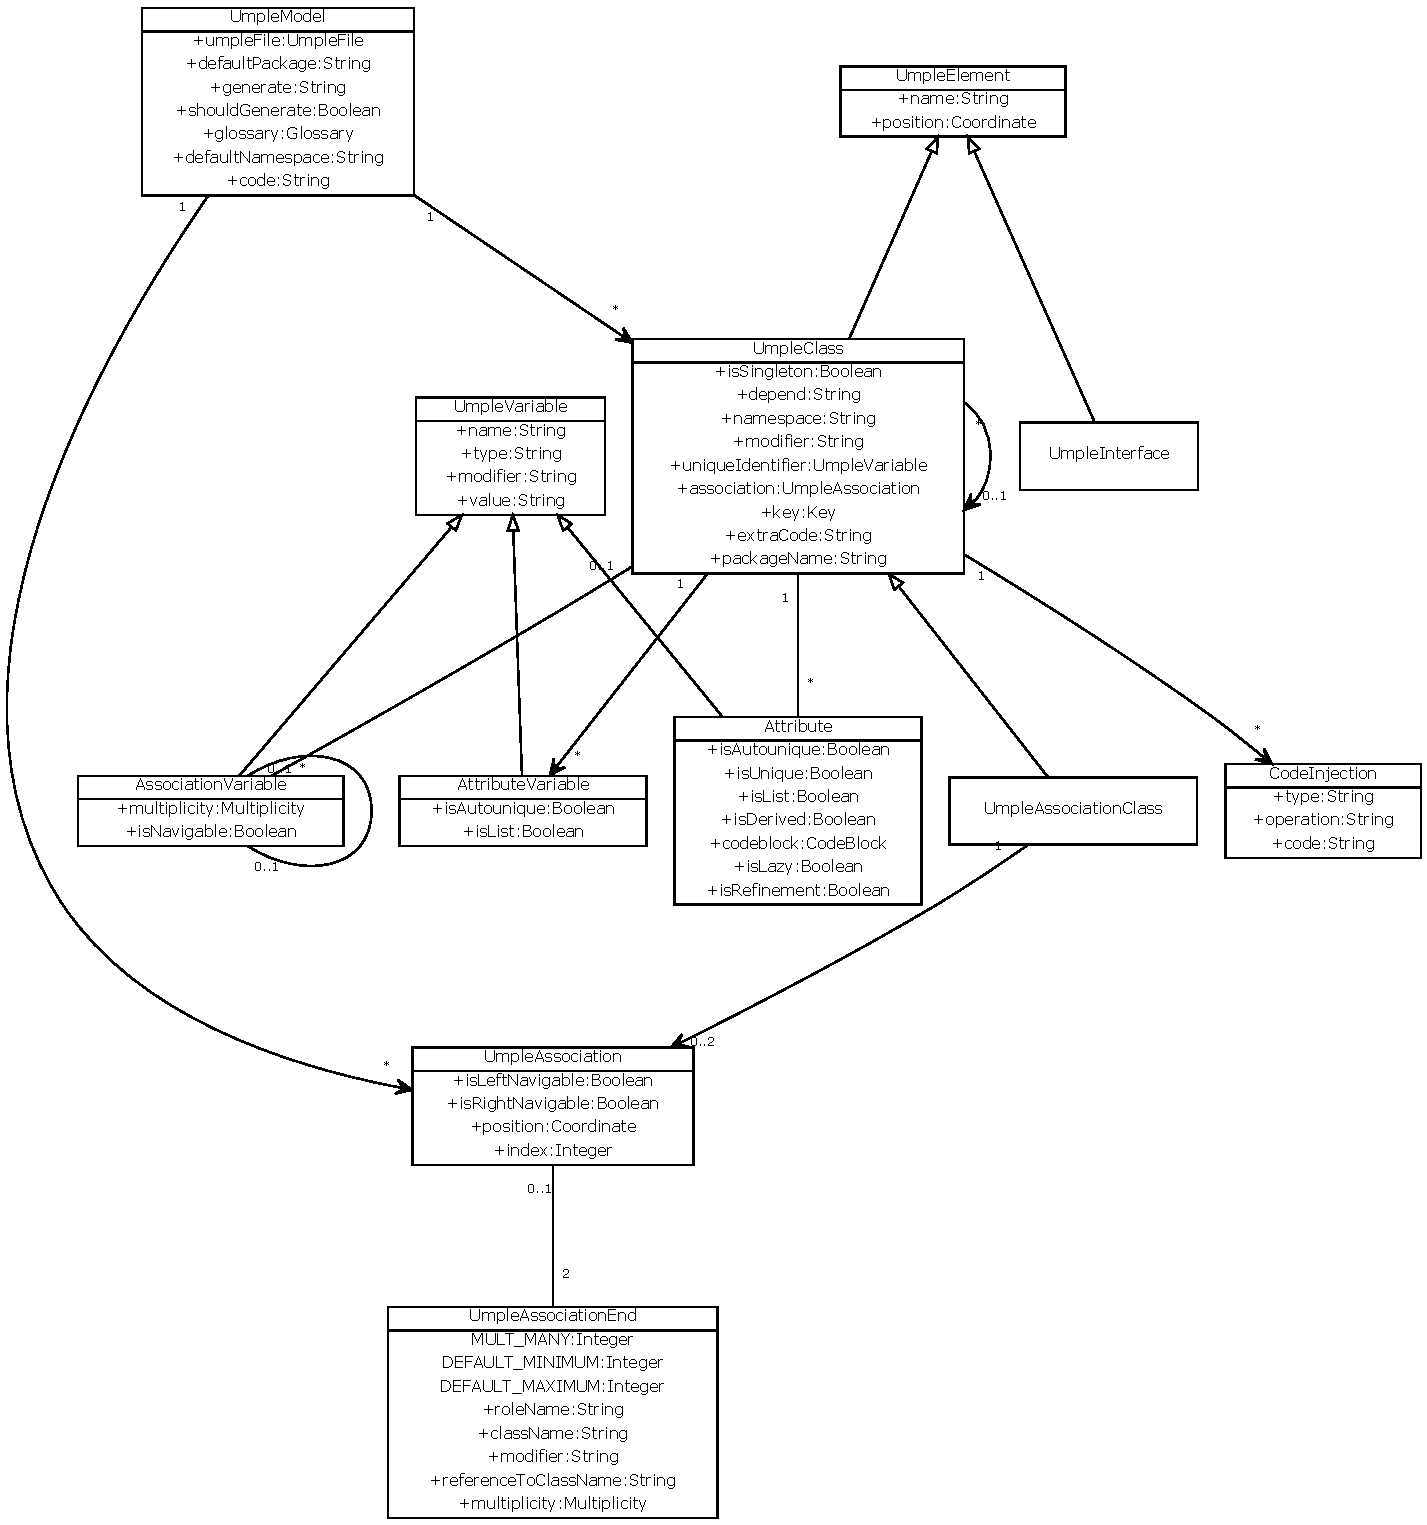
\includegraphics[width=1\textwidth]{Figures/metamodelUmple.pdf} 
\caption{Umple metamodel (partial)}
\label{fig:umpleMetamodel}
\end{figure}

\subsection{Umple Attributes}
\label{subsection:attributes}
An Umple attribute represents some information held by a class. For instance, 
a Person object might have a \textit{name} and an \textit{address}. 
An attribute can have various properties described in the following subsections.

\subsubsection{Basic Attributes}
A basic attribute in Umple represents simple data and is composed of one of the Umple data types and the name of the attribute. As shown in Tables \ref{table:apiAttrs1} and \ref{table:apiAttrs2}, the implications on code generation include a parameter in the constructor and simple set and get methods to manage access to the attribute. The String datatype in Umple is the default type, when no type is specified. The example in Listing \ref{lst:basicAttribute} shows multiple attributes having different (Umple) datatypes.

\begin{lstlisting}[style=umplePlain, label=lst:basicAttribute,caption=Basic Umple attribute]
class Demo 
{
  name; // String type
  Integer i;
  Float flt;
  String str;  
  Double dbl;
  Boolean bln;
  Date dte; 
  Time tme;
}
\end{lstlisting}

\subsubsection{Immutable Attributes}
The value of an immutable attribute cannot change during the lifetime of an instance of the class. The resulting base language code (e.g. Java) for an immutable attribute would be the same as the basic attribute implementation except that there would be not setter method generated. A constructor argument is required so the value can be set at construction time but  cannot be changed afterwards since no setter is generated. The syntax for an immutable attribute is shown in Listing \ref{lst:immutableAttribute}. In this example, the \textit{studentId} must be initialized during construction and cannot be changed after it. 
\newpage
\begin{lstlisting}[style=umplePlain,label=lst:immutableAttribute, caption=Immutable Umple attribute]
class Student 
{
immutable Integer studentId;
}
\end{lstlisting}

\subsubsection{Lazy and Immutable Attributes}
In cases where the attribute should be immutable, but the value is not available at the time of construction, the attribute can be declared as \textit{lazy immutable}. The use of the lazy syntax means that the attribute is not initialized in the constructor (i.e. it is not part of the constructor's signature). The generated code will contain a flag to track whether the object has been set yet, allowing only a single set to occur. In Listing \ref{lst:lazyimmutableAttribute},
attribute \textit{x} is declared as a lazy immutable attribute. The setter method of this attribute can be called once, since it will return false if we try to set it again (setter returns a boolean). Lazy immutable attributes are useful in architectures where the developer does not possess any control over the creation of the objects and therefore he cannot specify constructor arguments.

\begin{lstlisting}[style=umplePlain,label=lst:lazyimmutableAttribute, caption=Lazy immutable Umple attribute]
class A 
{
  lazy immutable x;
}
\end{lstlisting}


\subsubsection{Defaulted Attributes}
A defaulted attribute is set in the constructor to the default value, and can be reset to the default any time by calling a reset method (in this example \textit{resetName()}). It can be also set to any other value using its setter method. In Listing \ref{lst:defaultedAttribute}, the attribute 'name' is initializated to the default value 'UOttawa'. This default value can be queried by calling \textit{getDefaultName()}.

\begin{lstlisting}[style=umplePlain,label=lst:defaultedAttribute, caption=Defaulted Umple attribute]
class School 
{
  String name="UOttawa";
}
\end{lstlisting}

\subsubsection{Unique Attributes}
The unique attribute guarantees its uniqueness within a particular class.
For instance, in the example in Listing \ref{lst:uniqueAttribute}, in the set method of attribute `name', prior to setting its value, we will check for uniqueness. 

\begin{lstlisting}[style=umplePlain,label=lst:uniqueAttribute, caption=Unique Umple attribute]
class Student 
{
  unique String name;
}
\end{lstlisting}

\subsubsection{Autounique Attributes}
The implementation of autounique attributes is very similar to the implementation of unique attributes presented in the previous sub-section. The main difference is that the autounique attribute is set in the constructor to the next available value. Autounique attributes must be of type Integer as shown in Listing \ref{lst:autouniqueAttribute}.

\begin{lstlisting}[style=umplePlain,,label=lst:autouniqueAttribute, caption=Autonique umple attributes]
class Student 
{
  autounique Integer studentId;
}
\end{lstlisting}

\subsubsection{Constant Attributes}
A constant (class level) attribute is identified using the \textit{const} keyword as illustrated below. A constant is associated with the type itself, rather than an \textit{instance} of the type (i.e. it would be generated as a static variable in Java). Listing \ref{lst:constantAttribute} declares a constant of type Integer. 

\begin{lstlisting}[style=umplePlain,label=lst:constantAttribute, caption=Constants in Umple]
class Student 
{
  const Integer MAX_COURSES = 10;
}
\end{lstlisting}

\subsubsection{Array Attributes}
Umple supports attributes that might contain multiple values. The square brackets notation '[]' is used as illustrated in Listing \ref{lst:arrayAttribute}.

\begin{lstlisting}[style=umplePlain,label=lst:arrayAttribute, caption=Array attributes]
class Student 
{
  String[] nickname;
}
\end{lstlisting}

In translating Umple attributes into object-oriented programming languages such as Java, it is common to generate mutator and accessor methods. Tables \ref{table:apiAttrs1} and \ref{table:apiAttrs2} present the list of accessor and mutator methods generated from Umple attributes. In Tables \ref{table:apiAttrs1} and \ref{table:apiAttrs2}, T is the type of the attribute (String if omitted) and z is the attribute name.	

\begin{table}[h]
\centering
\caption{API generated methods from Umple attributes - Accessor  methods \cite{UmpleAPI}}
\label{table:apiAttrs1}
\begin{tabular}{lccc}
\toprule
\rowcolor[HTML]{BBDAFF}
\textbf{}               & \textbf{T getZ()}                                             & \textbf{boolean isZ()}     & \textbf{boolean equals(Object)} \\ \hline
      & returns the value                             & returns the value                                              & tests for reference equality    \\ \hline
\textbf{Basic}          & Yes                                                           & \begin{tabular}[c]{@{}l@{}}Yes;\\ if T is boolean\end{tabular} & No                              \\ \hline
\textbf{Initialized}    & Yes                                                           & \begin{tabular}[c]{@{}l@{}}Yes;\\ if T is boolean\end{tabular} & No                              \\ \hline
\textbf{Lazy}           & Yes                                                           & \begin{tabular}[c]{@{}l@{}}Yes;\\ if T is boolean\end{tabular} & No                              \\ \hline
\textbf{Defaulted}      & Yes                                                           & \begin{tabular}[c]{@{}l@{}}Yes;\\ if T is boolean\end{tabular} & No                              \\ \hline
\textbf{Immutable}      & Yes                                                           & \begin{tabular}[c]{@{}l@{}}Yes;\\ if T is boolean\end{tabular} & No                              \\ \hline
\textbf{Lazy immutable} & Yes                                                           & \begin{tabular}[c]{@{}l@{}}Yes;\\ if T is boolean\end{tabular} & No                              \\ \hline
\textbf{Autounique}     & \begin{tabular}[c]{@{}l@{}}Yes; \\ T always int.\end{tabular} & No                                                             & No                              \\ \hline
\textbf{Constant}       & No                                                            & No                                                             & No                              \\ \hline
\textbf{Internal}       & No                                                            & No                                                             & No                              \\ \hline
\textbf{Key}            & Yes                                                           & Yes                                                            & Yes                             \\ \hline
\end{tabular}
\end{table}

\begin{table}[h]
\centering
\caption{API generated methods from Umple attributes - Mutator methods \cite{UmpleAPI}}
\label{table:apiAttrs2}
\begin{tabular}{lcc}
\toprule
\rowcolor[HTML]{BBDAFF}
\textbf{}               & \textbf{boolean setZ(T)}                                  & \textbf{boolean resetZ()}                     \\ \hline
\textbf{Description}    & \multicolumn{1}{l}{mutates the attribute}                 & \multicolumn{1}{l}{restores original default} \\ \hline
\textbf{Basic}          & Yes                                                       & No                                            \\ \hline
\textbf{Initialized}    & Yes                                                       & No                                            \\ \hline
\textbf{Lazy}           & Yes                                                       & No                                            \\ \hline
\textbf{Defaulted}      & Yes                                                       & Yes;                                          \\ \hline
\textbf{Immutable}      & No                                                        & No                                            \\ \hline
\textbf{Lazy immutable} & \begin{tabular}[c]{@{}c@{}}Yes;\\ only once.\end{tabular} & No                                            \\ \hline
\textbf{Autounique}     & No                                                        & No                                            \\ \hline
\textbf{Constant}       & No                                                        & No                                            \\ \hline
\textbf{Internal}       & No                                                        & No                                            \\ \hline
\textbf{Key}            & Yes                                                       & No                                            \\ \hline
\end{tabular}
\end{table}

\subsection{Umple Associations}
\label{subsection:associations}
In Umple, as in UML, an association defines a relationship from a class to another class. Furthermore, it specifies which links, such as references or pointers, may exist at run time between the different instances of the classes.
More specifically, an Umple association is composed of the following information:

\begin{itemize}

\item \textit{Association Ends}: These are the classes involved in the relationship.

\item \textit{Navigability:} The navigability determines whether or not the association can be accessed from the opposite end. The notation '\--' is used when each class can access the linked objects of the other class and '-\textgreater{}' or '\textless{}-' to indicate that the navigation is possible in only one direction.

\item \textit{Multiplicity:} These are the restrictions on the numbers of objects allowed in the relationship.

\item \textit{Role names:} These are used to clarify the relationship and avoid name collisions if two classes are associated in multiple ways. Role names are optional except in reflexive associations or in other situations when name collisions might exist. The Umple compiler will give an error message if a role name is needed but absent.
\end{itemize}

The code segment in Listing \ref{lst:inlineAssoc} illustrates an association between instances of classes \emph{School} and \emph{Student}. In this example, an instance of class School can be associated to zero or more instances of class Student. The 'isA' notation is used to denote an inheritance relationship between the classes (Student is a subclass of Person). It should be noted that 'isA' is also used for other generalization relationships in Umple, such as implementation of Interfaces.

\begin{lstlisting}[style=umplePlain, caption=An example of an inline Umple association, label=lst:inlineAssoc]
class School {
 0..1 -- * Student student; //inline association
}
class Student {
  isA Person;
}
class Person { }
\end{lstlisting}

Alternatively, in addition to defining an association embedded in one of the associated classes, it is also possible to specify an association independently as shown in Listing \ref{lst:independentAssoc}. 

\begin{lstlisting}[style=umplePlain, caption=An example of an independent Umple association,label=lst:independentAssoc]
class School {
}
class Student {
  isA Person;
}
class Person { }

association {
 0..1 School -- * Student student;
}
\end{lstlisting}
Furthermore, Umple supports various kinds of associations as summarized below.
\paragraph{Reflexive}
An association in which both associations ends connect to the same class ~\cite{UMLSpec}. In other words, the class is associated to itself. In Listing \ref{lst:reflexiveAssoc}, the association is defined between Employee and itself, through the manager/manages role. The relationship means that an Employee in the role of manager can be associated with many managed Employees. 

\begin{lstlisting}[style=umplePlainNumbers, caption=A Reflexive association,label=lst:reflexiveAssoc]
class Employee {
0..1 manager -- * Employee manages ;
}
\end{lstlisting}

\paragraph*{Compositions}
A composition \cite{UMLSpec} is a sub-type of association where there is mandatory delete on the composition end, regardless of the multiplicity. 

The association in Listing \ref{lst:compositionAssoc} specifies that a Folder could contain many files, while each File has exactly one Folder parent. The composition constraint states that if a Folder (instance) is deleted, all contained Files (instances) are deleted as well.
\begin{lstlisting}[style=umplePlainNumbers, caption=A Composite association,label=lst:compositionAssoc]
class Folder { 
   1 parent <@>-* File files;
}
class File {}
\end{lstlisting}

\paragraph*{External}  
To associate a class to another class (external) that is not present or needs to be omitted from the compilation. External classes are useful when writing Umple code that will be connected to code written separately, such as code in a GUI library.
In Listing \ref{lst:externalAssoc}, class A is associated to class B which is not part of this model. Class B is shown as an external reference.
\begin{lstlisting}[style=umplePlainNumbers, caption=External associations,label=lst:externalAssoc]
class A {  
  1 -- 0..1 B; 
}  
external B {}
\end{lstlisting}

\paragraph*{Association Classes}
Association classes \cite{UMLSpec} define the features that do not belong to any of the connected classes but rather to the association itself. That is, a  shorthand for two one-to-many associations to a class that contains data that relates the two classes. The two related classes are logically in a many-many relationship. For instance, the association class in Listing \ref{lst:classAssoc} is used to gather the number of points a player gained on a particular team. 
\begin{lstlisting}[style=umplePlainNumbers, caption=An association class,label=lst:classAssoc]
class SportsPlayer {
  name;
}
class Team {
  name;
}
associationClass PlayerInTeam {
  Integer points;
  * SportsPlayer player;
  * Team team;
}
\end{lstlisting}

In Tables \ref{table:apiAssocs1} and \ref{table:apiAssocs2}, we show the generated API methods for accessing and mutating the links in the association. X is the name of the current class, W is the name of the class at the other association end and r is a role name used when referring to W.

\begin{table}[h]
\centering
\caption{API generated from Umple associations - Accessor methods \cite{UmpleAPI}}
\label{table:apiAssocs1}
\begin{tabular}{l|l}
\toprule
\rowcolor[HTML]{BBDAFF}
\textbf{Method Signature} & \textbf{Description}     \\ \midrule
W getW() & Return the W  \\ 
W getW(index) &	Picks a specific linked W  \\ 
List \textless W\textgreater getWs() & Gets immutable list of links  \\ 
boolean hasWs() & Returns true if cardinality is \textgreater  0 \\ 
int indexOfW(W)	 & Return index of W in the list\\ 
int numberOfWs() & Return the cardinality \\ 
\bottomrule
\end{tabular}
\end{table}

\begin{table}[h]
\centering
 \caption{API generated from Umple associations - Mutator methods \cite{UmpleAPI}}
\label{table:apiAssocs2}
\begin{tabular}{l|l}
\toprule
\rowcolor[HTML]{BBDAFF}
\textbf{Method Signature} & \textbf{Description}     \\ \midrule
boolean setW(W)   & Adds a link to existing W	\\ 
W addW(args)    & Constructs a new W and adds link      \\ 
boolean addW(W)  & Adds a link to existing W            \\ 
boolean setWs(W…)    & Adds a set of links              \\ 
 boolean removeW(W) &   Removes link to W if possible   \\
 \bottomrule
\end{tabular}
\end{table}
%TLFINAL removed semicolons above

\subsection{Code Injections}
Code injections are used to insert certain code statements \textbf{before} or \textbf{after} various Umple-defined actions on attributes, associations and (components of) state machines. Using \textbf{before} statements allows the developer to enforce preconditions, and using \textbf{after} statements to enforce postconditions or take actions based on the results of other actions. Code injections (after and before statements) can be added into the constructor, generated state machine event methods, any user-defined methods and into the API generated methods such as \textit{getX, setX, addX, removeX, getXs, numberOfXs, indexOfX}, where X is the name of the attribute or association.

\begin{lstlisting}[style=umpleOut,label={lst:codeInjection},caption=A code injection into the constructor]
class Operation {  
  const Boolean DEBUG=true;  
  query;  
  before constructor {  
    if (aQuery == null)  
    {  
      throw new RuntimeException("Please provide a valid query");  
    }  
  }  
  after constructor {  
    if (DEBUG) { System.out.println("Created " + query); }  
  }  
}  
\end{lstlisting}

The following gives details of the above:
\begin{itemize}
\item Line 2. Declares a constant (static final in Java). 
\item Line 3. Declares a simple (String) attribute.   	 
\item Line 4-9. Declares a code injection to be inserted at the beginning of the constructor.  
\item Line 10-12. Declares a code injection to be inserted at the end of the constructor.      
\end{itemize}

The code in Listing \ref{lst:codeInjection} generates the following (Java) constructor:

\begin{lstlisting}[style=java, caption=Generated constructor after code injection]
public Operation(String aQuery)
{
  if (aQuery == null)  
  {  
    throw new RuntimeException("Please provide a valid query");  
  }
  query = aQuery;
  if (DEBUG) { System.out.println("Created " + query); }
} 
\end{lstlisting}

\subsection{Umple Architecture and Tools}

The Umple compiler, which was originally written in Java, was fully rewritten in Umple in 2008, and has been developed and maintained in Umple since then. 

The compiler has a layered and pipelined architecture as shown in Figure \ref{fig:umpleArchitecture}. 
The components of Umple include: a parser, an analyzer as well as several code generators and model-to-model transformation engines. These are described below:

\begin{enumerate}
\item \textbf{Parser}: The parser receives an input model, written in Umple (with code in other languages mixed in), tokenizes it and passes it to the next component in the pipeline.

\item \textbf{Analyzer}: This component processes the tokens previously obtained and converts them into an internal representation consistent with Umple's metamodel (instances of the metamodel classes). Errors and warnings are produced at this stage. Warnings mean that generation can occur, but there may be issues with the generated result. Errors mean that no code generation will be possible.

\item \textbf{Code-Generator(s)}: The internal representation is then translated into other artifacts; either additional models like Papyrus XMI, Ecore, Yuml; various diagrams, or source code such as Java, C++, PHP, Ruby or SQL. The compiler generates various types of methods including mutators (to control changes to a variable) and accessors (to return the value of a variable) from the various Umple features. Sophisticated code for managing state machines, tracing \cite{UmpleTracing}, generation templates, patterns, aspects and concurrency can also be generated from models.

\end{enumerate}
\begin{figure}[h]
\centering
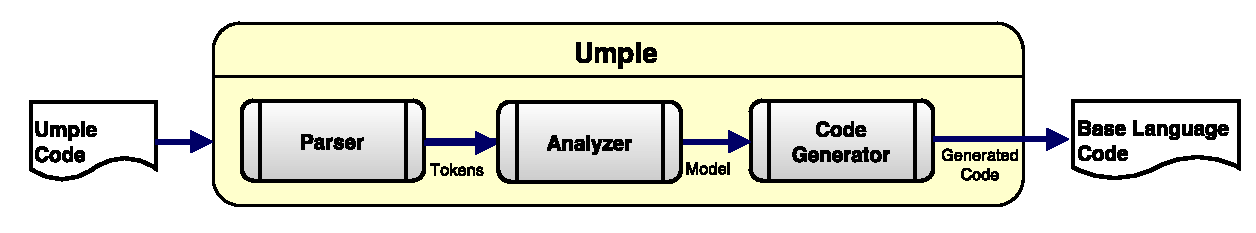
\includegraphics[width=0.99\textwidth]{Figures/umpleArchitecture.pdf} 
\caption{Umple architecture}
\label{fig:umpleArchitecture}
\end{figure}

Each component is tested independently to ensure that the input is processed correctly and the output produced is valid ~\cite{umpleTesting2014}. Testing the Umple parser is centered on tokenization of Umple code. Testing the metamodel classes ensures that the analyzer component produces valid metamodel instances. Testing of generated systems is also performed.

In addition to the Eclipse plugin and command-line based compiler, UmpleOnline \cite{UmpleOnline}, a web-based application shown in Figure \ref{fig:uonline}, allows to instantly experiment with Umple on the Web. 

\begin{figure}[h]
\centering
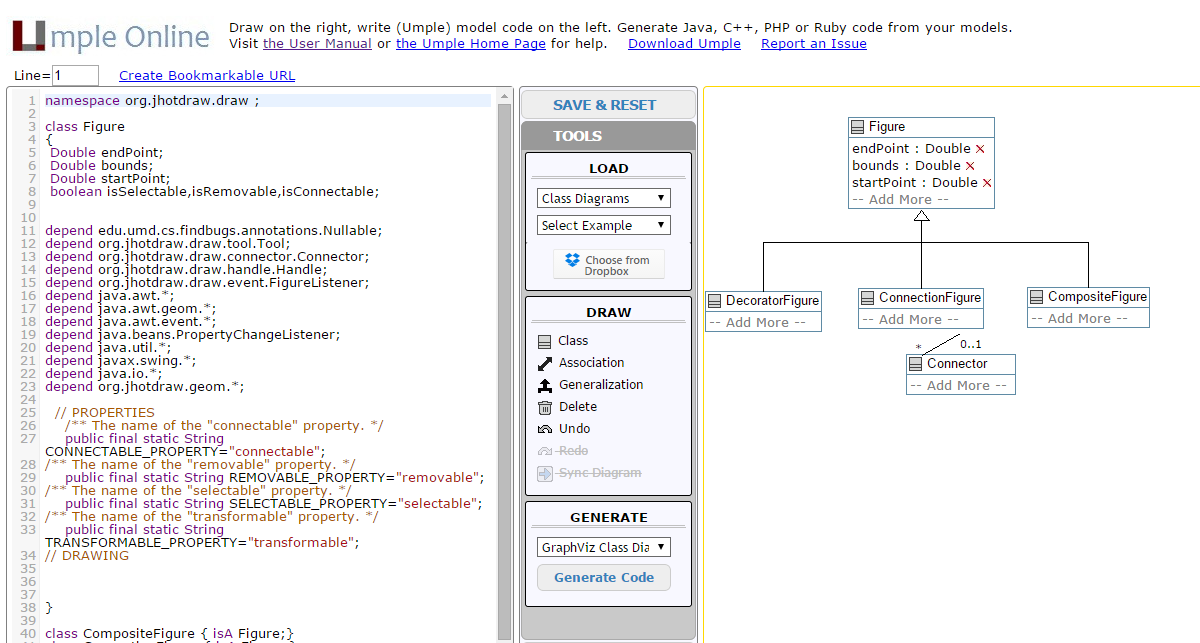
\includegraphics[width=0.75\textwidth]{Figures/uonline.png} 
\caption{Umple online}
\label{fig:uonline}
\end{figure}


\section{Transformations}

In this section we will describe the different transformations that can occur during software design and implementation activities that are relevant to our research. In particular, we will present transformations that can occur during the design phase, during the implementation phase and when moving from one phase to another. Forward engineering, reverse engineering, model transformations and refactorings will be introduced in the following sections. The different transformations enumerated above are relevant to our work for the following reasons: 

\begin{itemize}
\item The umplification approach presented in this thesis is a \textit{reverse engineering} technique performing \textit{model transformations} to transform a base language model into an Umple model. 
\item The output of umplification is an Umple model. Umple models can be used to generate high quality code (\textit{forward engineering}).
\item \textit{Refactorings} by means of umple code injections are required to adapt the different methods of an input class to conform to the Umple generated methods.
\item The umplification approach can be used in some measure to re-engineer an existing software system. A case study presenting a modernized software system is studied in the last section of Chapter \ref{chap:evaluation}.
\end{itemize}

To better conceptualize the different transformations, it is necessary to place them in the larger context of the software system lifecycle. As described in \cite{Chikofsky} and illustrated in Figure \ref{fig:reveng}, we assume a software life cycle with three main stages: Requirements, Design and Implementation (even in an agile approach, these would occur, though in tight iterations). In the requirements phase, the problem being solved is specified, in the design phase the solution is specified using a well-defined model and in the implementation phase the code is produced from the previously obtained model. The work presented in this thesis as well as the related work studied focuses exclusively on the transformation that occur in the two last (abstract) stages of the life-cycle. Figure \ref{fig:reveng} has been taken from \cite{Chikofsky} but has been simplified and modified for our purposes. As illustrated in Figure \ref{fig:reveng}, the level of abstraction is higher in early stages and lower in later stages. Five different types of transformations can be distinguished:

\begin{figure}[h]
\centering
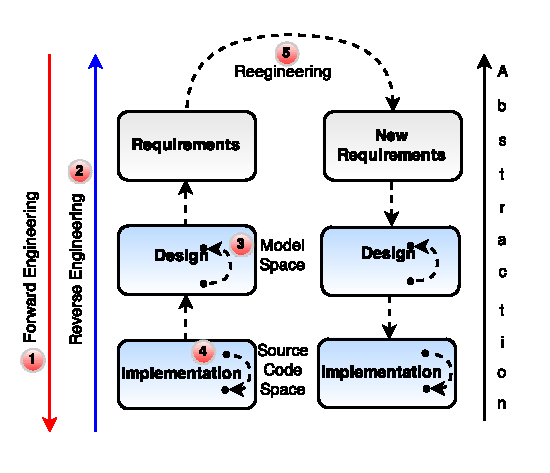
\includegraphics{Figures/transformationsRE}
\caption{Transformations across the different software life-cycle phases}
\label{fig:reveng}
\end{figure}

\begin{enumerate}
\item \textit{Forward engineering} produces source code corresponding to an object model. The modeling constructs in the model such as attributes, associations and high-level constraints, are automatically mapped to source code constructs supported by the selected programming language. 

\item \textit{Reverse engineering} produces a model corresponding to source code. This transformation is often applied when the design of the system has been lost and must be recovered. Reverse engineering can be seen as going backwards through the development cycle. Furthermore, reverse engineering does not involve changing aspects of the subject system. 

\item \textit{Model transformations} involve a conversion of an object model into another object model. 

\item \textit{Refactorings} involve transformations that operate on source code elements. Their goal is to improve aspects of the system without changing its functionality. They operate in the source code space.
\item \textit{Re-engineering} produces a new form of the subject system. 
\end{enumerate}

\subsection{Forward Engineering}

In Forward Engineering the target system is created by moving down from high-level abstractions to logic design and proceeds to the physical design of the system. The main goal of forward engineering is to maintain a strong correspondence between the object design model and the code and to reduce the development effort. 

\begin{quote} 
``Forward engineering is the traditional process of moving from high-level abstractions and logical, implementation-independent designs to the physical implementation of a system.'' \cite{Chikofsky}
\end{quote} 

Examples of forward engineering transformations include:

\begin{description}

\item [Mapping UML classes to base language classes:]
Classes in the well-defined model (UML, Umple) are taken one by one and mapped into classes in the target programming language. 

\item [Mapping attributes to member variables and related code:]
Attributes in the model are mapped into member variables according to their characteristics. Implications on code generation in a object-oriented language such as Java, include a parameter in the constructor and mutator and accessor methods to manage access to the attribute.

\item [Mapping associations to variables, collections, and related code:]
Associations, model concepts representing links between two or more objects are mapped into member variables and methods. Object-oriented programming languages do not support directly the concept of associations, they provide references to objects that can be stored. Associations are then realized in terms of references, taking into account the different parts of an association such as the role name, multiplicities and navigability. 

\item [Mapping constraints to Exceptions or other types of code:]
Model constraints expressed in the model in \textit{OCL} or in natural language are mapped to code that checks the preconditions, postconditions and invariants in the target programming language.

\item [Mapping Object models to a persistent storage schema:]
Object model is mapped to a storage schema. Attributes of the object models are mapped into columns and associations between the objects are mapped using a combination of primary and foreign keys. 
\end{description}

\subsection{Reverse Engineering}

Reverse engineering, which involves extracting design artifacts and recovering models that are less implementation-dependent, has been defined by Chikofsky and Cross \cite{Chikofsky} as:

\begin{quote} 
``the process of analyzing a subject system to
\begin{itemize}
\item identify the system's components and their interrelationships and
\item create representation of the system in another form or at a higher level of abstraction''.
\end{itemize}
\end{quote}

Reverse-engineering is generally used to:
\begin{itemize}
\item Cope with complexity: understand large and complex systems.
\item Generate alternative views: automatically generate different ways to view systems
\item Recover lost information: extract what changes have been made and the reasons for those changes.
\item Detect side effects: help understand ramifications of changes.
\item Synthesize higher abstractions:  create alternative views that transcend to higher abstraction-level software.
\item Facilitate reuse: detect candidate reusable artifacts and components.
\end{itemize}

The umplification process can be used to do all of these, but in particular to synthesize higher abstractions.

Table \ref{table:approachesRE} summarizes another categorization  of reverse engineering approaches \cite{Chikofsky}. Umplification includes design recovery, restructuring, refactoring, and a certain amount of data re-engineering.

\begin{table}[h]
\centering
\caption{Summary of Reverse engineering approaches \cite{Chikofsky}}
\label{table:approachesRE}
\begin{tabular}{l|p{6cm}|p{4cm}}
\toprule
\rowcolor[HTML]{BBDAFF}
\textbf{Approach} & \textbf{Description}  & \textbf{Related Techniques}  \\ \midrule
Re-documentation 
&  The creation or revision of a semantically equivalent representation within the same relative abstraction level. 
& Pretty printers, diagram generators, reference listing generators.\\ \hline

Design recovery & Extracts design abstractions from a combination of code and existing documentation of the system. & Software metrics generators, static analyzers, dynamic tracers, visualization tools. \\ \hline

Restructuring & The transformation from one representation form to another at the same relative  abstraction level, while preserving the system's external behavior & Source code analyzers, source code translators.   \\ \hline

Data re-engineering & The process of analyzing and is the process of analyzing and
reorganizing the data structures (and sometimes the data values) in a system to make it more understandable & Data model analyzers  \\ \hline
Refactorings & Small scale restructuring & Refactoring APIs \\ 
\bottomrule 
\end{tabular}
\end{table}

\subsection{Model Transformations}

Model transformation is a method that allows the automation of many activities like reverse engineering, refactoring, integration, analysis and simulation \cite{biehl2010literature}, which are used extensively in software development, maintenance and modernization. Model transformations are employed in tools such as code generators and parsers as well.

Kleppe et al. \cite{mccKleppe} provide a more formal definition of a model transformation:


\begin{quote}
``A \textit{transformation} is the automatic generation of a target model from a source model, according to a transformation definition. 
\end{quote}
\begin{quote}
A transformation \textit{definition} is a set of transformation rules that together describe how a model in the source language can be transformed into a model in the target language.
\end{quote}
\begin{quote}
A transformation \textit{rule} is a description of how one or more constructs in the source language can be transformed into one or more constructs in the target language.''
\end{quote}

Model transformations provide a mechanism for automatically creating or updating target models based on information contained in a source model, e.g. the generation of code from a UML model, the translation of a UML Class Diagram into an ER (entity-relationship) diagram or the translation of base language code into UML or any other textual or visual modeling language, such as Umple.

In order to perform a transformation between models, the models need to be expressed in a software language. This language can be specified by a \textit{grammar} or a \textit{metamodel}. As stated by Kleppe \cite{kleppe2007language}, grammars focus on the concrete syntax of the language while metamodels focus on the abstract syntax.

Grammars are useful to describe the structure of the words in a language, metamodels are better in describing the language's concepts and its relations. Compared to metamodels, grammars have a strong mathematical basis (induction can be used to prove correctness) and are tree based (e.g., parse trees are generated from them). Also, there are a great variety of  advanced tools to produce, parse and validate grammars.

On the other hand, metamodels are graph based in which relations between language elements are better perceived. Moreover, metamodels are more suitable when defining object-oriented languages but do not contain information on how the concepts in the metamodel are to be represented to the language user \cite{kleppe2007language}. Nevertheless, as studied by Alanen et al. \cite{alanen2003} it is possible to transform a grammar definition into a metamodel definition and vice-versa. In fact, the relation between a metamodel and a BNF grammar can in practise be defined using two mappings, one transforming a BNF grammar to a MOF metamodel,
and one transforming a MOF metamodel to a BNF grammar.

Previous work \cite{Czarnecki2006, biehl2010literature} on model transformations allows us to conclude that no existing model transformation tool or technique is \textit{absolutely} better than another one. Instead we can search for a model transformation approach that is suitable for a specific transformation problem. The following are the main properties of model transformation problems \cite{biehl2010literature}:

\begin{itemize}

\item Change of abstraction: Model transformations can change the level of abstraction between the source and the target model. That is, the transformation increases or decreases the level of detail or leaves it unchanged.

\item Change of Metamodel: 
	\begin{itemize}
		\item In an \textit{endogenous} \cite{Visser2005} transformation, both the source and target metamodels are the same.
		\item In an \textit{exogenous} \cite{Visser2005} transformation,  the source and target metamodels are 			different.
	\end{itemize}
\item Supported technical spaces: Model transformations can operate between the metametamodel, metamodel and model levels \cite{OOPSLA2004Bezivin}. 

\item Supported number of models: A transformation can involve one model (same source model resulting in a modified target model), two models (source and target models are different) and multiple models (several source models that produce a single target model).

\item Supported target type: The target model can be either text or another model. A Model-to-Text transformation creates its target as a set of strings while a  Model-to-Model transformation creates its target as an instance of the target metamodel.

\item Preservation of properties: Transformations can be performed in such a way that the source and target models have a common property that is not transformed by the transformation \cite{biehl2010literature}. The intent of that common property can be to preserve the semantics, syntax or behavior of the source and target models. 
\end{itemize}

Based on the target type supported, we categorized the model transformation approaches into two major categories \cite{Czarnecki2006}: Model-to-Model and Model-to-Text approaches. 

\subsubsection{Model-To-Text Approaches}
\begin{description}

\item[Visitor-Based Approaches:]
An approach based on the notion of traversing the internal representation of the model. The output is written to a text stream. The approach is based on the Visitor software pattern \cite{gamma1994design}. 

\item[Template-Based Approaches:]
Template-based approaches are used in the implementation of code generators. The basic idea is to refine and transform models into code. The templates contain fragments of the target text and pieces of code that are replaced with information derived from the source model (called meta-programs). This approach can be combined with the visitor-based approach for model traversing. 
\end{description}

\subsubsection{Model-To-Model Approaches}
\begin{description}

\item[Direct-Manipulation Approaches:] The approach typically consists of an internal representation of the model (e.g. AST) and some API's to manipulate and query it. The Modisco \cite{ModiscoMain} technology falls under this category.

\item[Structure-Driven Approaches:]
The basic idea behind this approach is to copy model elements from the source to the target, which can  then be adapted to achieve the transformations goals. The approach is structure-driven because this approach first creates the hierarchical structure of the target model. The \textit{OptimaJ} framework is one of the representative technologies falling under this category.

\item[Operational Approaches:]
Operational approaches extend the metamodeling formalism with facilities for expressing mapping rules. 
Imperative approaches focus on how the transformation itself needs to be performed. Operational transformation languages provide support to describe how the transformation language is supposed to be executed. The constructs and concepts of an imperative language are similar to those of general purpose programming languages such as Java. The model transformation in this case is described as an ordered sequence of actions. \textit{Kermeta} and \textit{QVT}, presented later in this chapter, are examples of technologies in this category.

\item[Declarative Approaches:]
Declarative approaches do not offer explicit control flow. They do not describe how the transformation should be executed but instead what should be mapped by the transformation. In other words, they describe the relationship between the source and the target metamodels. The transformation descriptions (or mapping rules) for these languages are, in general, short and concise. 

\item[Hybrid Approaches:]
Hybrid transformation languages are a mix of declarative and operational approaches and offer the possibility of declaring how and what elements of the metamodels are going to be mapped \cite{HybridModelTransform}.

\item[Graph-Transformation-Based Approaches:]
Graph-based approaches can be considered as a special subcategory of declarative languages. Models are interpreted as graphs, and the transformation manipulates these graphs \cite{GraphTransformations2006}. For instance, the Triple Graph Grammar (TGG) \cite{GraphTransformations2006} is a way of describing graph transformations. Their rules are specified using three graphs, the left-hand side graph corresponding to the source graph, the right-hand side graph corresponding to the target graph and a correspondence graph describing the mapping between elements of the left-hand side and elements of the right-hand side.

\item[XML Approaches:]
In this approach models are serialized as XML and then traversed and transformed using XSLT or similar technology. However, the use of XMI and XSLT has scalability limitations \cite{peltier2001mtrans}. 
\end{description}

\subsubsection{Model Transformations Languages and Tools}

We now introduce some of the most popular existing model transformation technologies.

\begin{description}
\item[ATL]
The ATLAS Transformation Language \cite{atl} is a hybrid model-to-model trans-formation language supporting both declarative and imperative constructs. ATL is integrated in the Eclipse development environment and can handle models based on EMF (Ecore). The ATL code (.atl files) is compiled and then executed by its own transformation engine. Examples of Java-to-Umple ATL transformations will be presented in Chapter \ref{chap:tool}.

\item[QVT]
The Query/View/Transformation \cite{QVTMain} is a standardized language for model transformation established by the Object Management Group (OMG). QVT defines three syntaxes for model-to-model transformations: a textual concrete syntax, an XMI-based metamodel and visual syntax for matching element between metamodels.
Listing \ref{lst:QVTExample} shows a partial transformation from a UML class model to an Umple model.

\begin{lstlisting}[style=java,label=lst:QVTExample, caption=A basic QVT transformation]
transformation uml2Umple(
 in uml : SimpleUML,
 out umple : SimpleUmple
);

main() {
  uml.objectsOfType(Class)->map UMLClassToUmpleClass();
}

mapping Class::classToUmpleClass () : UmpleClass
{
  name := self.name;
  attributes : self.attributes->map attributeToUAttribute();
}

mapping Attributes::attributeToUAttribute () : Attribute {
 ... omitted
}
\end{lstlisting}

The following gives details of the above:

\begin{itemize}

\item Lines 1-4. The transformation declaration specifies the parameter models. The transformation is unidirectional from UML to Umple.

\item Line 6. The entry point for the execution is the function \textit{main()}, which invokes the \textit{UMLClassToUmpleClass} mapping on all UML classes. 

\item Lines 10 and 16. The mappings are defined using the OCL notation. The attributes of each UML class are traversed and converted to Umple attributes (code is omitted). The body of the mapping populates the properties of the return object, while self refers to the object on which the mapping is invoked.
\end{itemize}

\item[JET]
Java Emitter Templates (JET) is a generic template engine that can be used to generate SQL, XML, Java source code and other output from templates. The templates uses a JSP-like syntax.
For instance, the code in Listing \ref{lst:JETExample} will print the words "Hello, Thesis Reader!" to the standard console output. The JET Builder translates the template to a class named BasicTemplate. The template file receives a string argument.

% I don't see a reference to Jet

\begin{lstlisting}[style=java,label=lst:JETExample, caption=A basic JET Template]
<%@ jet package="hello" class="BasicTemplate" %>
 Hello, <%=argument%>!
\end{lstlisting}

To pass arguments to the template method, we use the generate \textit{method} as shown in Listing \ref{lst:JETExample2}. Note that it is possible to pass a reference (a model element) type as argument. 

\begin{lstlisting}[style=java,label=lst:JETExample2, caption=Instantiating the BasicTemplate class]
 BasicTemplate sayHello = new BasicTemplate();
 String result = sayHello.generate("Thesis Reader");
 System.out.println(result);
\end{lstlisting}

\item[Kermeta]
Kermeta \cite{kermetaMain} is an imperative programming language used to perform model transformations and for other more general purposes. It offers EMF meta-modeling, checks and behavior support. Incremental model transformations are supported. The Kermeta language uses metamodel-based actions to manipulate elements from different metamodels (in XMI format) and transform them. 

\item[ETL]
ETL \cite{ETLMain}  is a hybrid model-to-model transformation language. It can handle several source and several target models. It offers support for query/navigate/modify both source and target models. It works at the metamodel level and supports EMF models. 

\item[TXL]
TXL \cite{Cordy2006}  is a programming language designed for a variety of analysis and source transformation tasks. TXL is a hybrid rule-based language and it is best at tasks involving source-to-source transformations.  Examples of Java-to-Umple TXL transformations will be presented in Chapter \ref{chap:tool}.
\end{description}

Table \ref{table:toolSummary} summarizes the most representative tools for each model transformation approach discussed.

\begin{table}[h]
\centering
\caption{Summary of model transformation technologies}\label{table:toolSummary}
\begin{tabular}{l|p{6cm}}
\toprule
\rowcolor[HTML]{BBDAFF}
\textbf{Tranformation Approach} & \textbf{Technologies}     \\  \midrule
M2T- Visitor-Based Approaches & Jamada, CodeWirters  \\  \\ \hline
M2T- Template-Based Approaches  & JET, Velocity, XDoclet, Codagen  \\ \\ \hline
\hline
Direct-Manipulation Approaches & JML   \\ \hline
Structure-Driven Approaches & QVT, OptimalJ   \\ \hline
Operational Approaches & XMF-Mosaic, QVT-Relational, Kermeta  \\ \hline
Declarative Approaches & ATL, ETL    \\ \hline
Hybrid Approaches & CSCWMDA   \\ \hline
Graph-Based Approaches & AGG, AToM3, VIATRA, GReAT, UMLX, BOTL, MOLA, and Fujaba  \\ \hline
XML Approaches & XSLT   \\ 
\bottomrule
\end{tabular}
\end{table}

\subsection{Refactorings}

A \textit{refactoring} is a transformation of the \textit{source code} aiming at improving its readability and/or design of the code without changing the behavior of the system \cite{Fowler2000}. To ensure that the refactoring does not change the behavior of the system, the refactoring is done in small incremental steps that are interleaved with tests. 
For example, a sequence of three refactorings are performed to the source code in Listing \ref{lst:refactoring}.
The resulting source code after the transformations is presented in Listing  \ref{lst:refactoring2}. The refactorings are performed one by one, ensuring that the refactoring does not change the intended behavior of the system. For a complete catalog of  refactorings refer to \cite{Fowler2000}. 

\begin{enumerate}
\item Pull Up Field: Common field in subclasses is moved to the superclass. In our example, field \textit{name} is moved to superclass. 
\item Pull up Constructor: Common code in constructor bodies of subclasses is moved to the superclass constructor. 
\item Pull up Method: Methods with identical results on subclasses are moved to superclass. In our example, the methods accessing the \textit{name} field are moved from the subclasses to the superclass. 
\end{enumerate}


\noindent\begin{minipage}{.45\textwidth}
\begin{lstlisting}[style=java,caption=Before refactorings,label=lst:refactoring]{Name}
public class Student {
  private String name;
  public Student(String name) {
   this.name = name;
  }
  public String getName() {
	return name;
  }
}
///----- Class Mentor ------
public class Mentor {
  private String name;
  public Mentor(String name) {
   this.name = name;
  }
  public String getName() {
	return name;
  }
}
\end{lstlisting}
\end{minipage}\hfill
\begin{minipage}{.45\textwidth}
\begin{lstlisting}[style=java,caption=After refactorings,label=lst:refactoring2]{Name2}
///----- SuperClass ------
public class Person {
  private String name;
  public Person(String name) {
   this.name = name;
  }
  public String getName() {
	return name;
  }
}
///----- Class Student ------
public class Student extends Person {
  private String name;
  public Student(String name) {
   super(name);
  }
}
///----- Class Mentor ------
public class Mentor extends Person {
  private String name;
  public Mentor(String name) {
   super(name);
  }
}
\end{lstlisting}
\end{minipage}

\subsection{Re-engineering}

Re-engineering is the examination and alteration of a subject system to reconstitute it in a new form \cite{Chikofsky}. 
Re-engineering transformations are usually concerned with reimplementing a system (or parts of it) to make it more maintainable. Re-engineering involves redocumenting the system, organizing and restructuring the system or translating the system to a more modern programming language, know as modernization. Modernization is performed to extract the main components of the system, written in old (legacy) code, and to reproduce the original system using a more recent programming language or using modern frameworks and libraries.

The main activities in a typical re-engineering process are:

\begin{description}
\item[Source Code Translation:]
The most simple form of re-engineering is source code translation and involves the automatic translation of source code written in one programming language to source code in another (i.e., C to C++). The translation should not modify the structure and organization of the system. Source code translation can be done to the same but more modern version of the language (i.e., Java 1.4 to Java 1.8). A source code translation is very desirable when the language compiler or support is discontinued or when the organization policies impose a change on the language (i.e., Microsoft technologies to open source technologies). Furthermore, systems written in modern languages are often easier to understand, test and maintain than legacy systems \cite{Pressman2001}.

\item[Reverse Engineering:]
Reverse engineering can be used as part of the reengineering process to recover the original program design. The design can then help developers understand the program internals before attempting to improve it. As originally explained by Chikofsky  \cite{Chikofsky}, reverse engineering and reengineering differ in their purpose. The main goal of reverse engineering is to derive the specification or design of a system from its source code, while the purpose of reengineering is to produce a new but more maintainable system. 

\item[Program Improvements:]
This part of the reengineering process involves improving the structure of the program to optimize memory use or to simplify the logic structure of the system. 
\end{description}

\section{Summary}

Umple is a modeling and programming language that incorporates UML concepts. We have focused our discussion about Umple classes, attributes, associations and code injections. This chapter analyzed the syntax of attributes and associations and presented the code generation patterns when these Umple constructs are translated into Java. Furthermore, we provided an overview of the tools currently available to support the creation of Umple systems; as well as the Umple Grammar, metamodel and architecture.

A wide range of reverse engineering and modeling transformation techniques and tools were introduced in this chapter. Both are required to understand the core concept of this thesis, the umplification technique, a reverse engineering technique that employs model-to-model transformations to  incrementally transform base language code into Umple code. The umplification technique will be described in the next chapter. % Background  

\lhead{\emph{\leftmark}} 
\chapter{Reverse Engineering of Object Oriented Systems into Umple}
\label{chap:core}

In this chapter we provide an overview of our reverse-engineering technique, called \textit{umplification}. Then, we discuss our motivations for developing the umplification technique and present a comprehensive example. 

\section{Umplification Process}

\textit{Umplification} is a play on words with the concept of `amplification' and also the notion of converting into Umple. The technique produces a program with behavior identical to the original one, but written in Umple. The umplification process is incrementally performed until the desired level of abstraction is achieved. 

The purposes of umplification include a) allowing the user to better understand their system, since the model becomes visible; b) reducing code volume by generating code that would otherwise be repetitive; c) allowing the developer to switch to model-driven development from that point onwards, and to use the modeling abstractions found in Umple more fully.

\subsection{Description}
Umplification, as illustrated in Figure \ref{fig:umplificationLoop}, involves recursively modifying the Umple model/code or the base language code to incorporate additional abstractions, while maintaining the semantics of the program, and also maintaining, to the greatest extent possible, such elements as layout. The end product of umplification is an Umple program/model that can be edited and viewed textually just like the original program, and also diagrammatically, using Umple's tools. 

\begin{figure}[h]
\centering
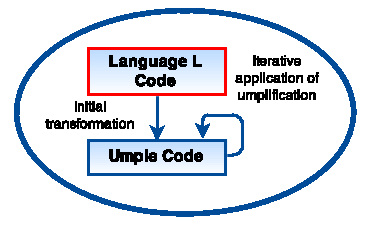
\includegraphics[width=0.50\textwidth]{Figures/UmplificationProcess.pdf}
\caption{The Umplification process generalized}
\label{fig:umplificationLoop}
\end{figure}

\subsection{Properties}

The umplification process has several properties. It is:
\begin{enumerate}
 \item \textbf{incremental}, 
 \item \textbf{transformational},
 \item \textbf{interactive},  
 \item \textbf{extensible}, and
 \item \textbf{implicit-knowledge} conserving. 
\end{enumerate}

The approach is \textbf{incremental} because it can be performed in multiple small steps that produce (quickly) a new version of the system that has a small amount of additional modeling information, such as the presence of one new type of UML/Umple construct. At each step, the system remains compilable. The approach proceeds incrementally performing additional transformations until the desired level of abstraction is achieved.	These incremental transformations allow for user interaction to provide needed information that may be missing or hard to automatically obtain because the input (the source code) does not follow any of the idioms the automatic umplification tool is yet able to recognize.
%FINAL CHANGE START - Clarifying the mess I did on the incrementality concept.
This characteristic of umplification allows developers, if they wish, to repeatedly re-introspect the transformed program and manually validate each change with an understanding of the incremental purpose of the change. From a technical perspective, incrementality is reflected in the fact that the tool implementing our approach accepts Umple as input. That is, an Umple model with a higher level of abstraction can be recovered from an Umple model containing fewer umplified constructs. 
%FINAL CHANGE END
%TLFINAL - minor adjustment made

The approach is \textbf{transformational} because it modifies the original source rather than generating something completely new. It first translates the original language (Java, C++ etc.) to an initial Umple version that looks very much like the original, and then translates step-by-step as more and more modeling constructs are added, replacing original code.

The approach is \textbf{interactive} because the user's feedback may be used to enhance the transformations.

The approach is \textbf{extensible} because the set of transformation rules it uses can be readily extended to refine the transformation mechanism. 

Finally the approach is \textbf{implicit-knowledge} conserving because it preserves code comments, and, where possible, the layout of whatever code is not (yet) umplified. The latter includes the bodies of algorithmic methods – known as \textit{action code} in UML.

Taken together, the above properties allow developers to confidently umplify their systems without worrying about losing their mental model of the source code. Developers gain by having systems with a smaller body of source code that is intrinsically self-documented in UML. 

\subsection{Overview of Transformations Cases}
\label{subsection:overview}
The following gives a summary of the abstract transformations currently implemented. 
\begin{description} 
\item[Transformation 0: Initial transformation] 
Source files written in language L (e.g. Java, C++) are initially renamed as Umple files, with extension .ump. File, package and data type dependencies are translated into Umple dependencies by using the Umple depend construct. 

\item [Transformation 1: Transformation of generalization/specialization, and namespace declarations]
The notation in the base language code for subclassing is transformed into the Umple `isA' notation. Umple now recognizes the class hierarchy. Notations for namespaces or packages are transformed into the Umple `namespace' directives. At this stage, an Umple program, when compiled should generate essentially code identical to the original program.

\item [Transformation 2: Analysis and conversion of many instance variables, along with the methods that use the variables]
This transformation step is further decomposed into sub-steps depending on the abstract use of the variables. The sub-steps are defined as follows.
	\begin{description}

	\item [Transformation 2a: Transformation of variables to UML/Umple attributes]
	If variable \textit{a} is declared in class A and the type of \textit{a} is one of the primitive types in the base language, then \textit{a} is transformed into an Umple attribute. Any accessor (e.g. getA()) and mutator (e.g. setA(…)) methods of variable \textit{a} are transformed as needed to maintain a functioning system. In particular, any getter and setter methods in the original system must be adapted to conform to or call the Umple-generated equivalents.
	
	\item [Transformation 2b: Transformation of variables in one or more classes to UML/Umple associations]
	If variable \textit{a} is declared in Class A and the type of \textit{a} is a reference type B, then \textit{a} is transformed into an Umple Association with ends \{a, b\}. At the same time, if a variable \textit{b} in class B is detected that represents the inverse relationship, then the association becomes bidirectional. The accessor and mutator methods of variable \textit{a} (and \textit{b}) are adapted to conform to the Umple-generated methods. Multiplicities and role names are recovered by inspecting both types A and B.

	\item [Transformation 2c: Transformation of variables to UML/Umple state machines]
	If \textit{a} is declared in Class A, has not been classified previously as an attribute or association, has a fixed set of values, and changes in the values are triggered by events, and not by a set method, then a is transformed to a state machine.
% FINAL CHANGE START
We will not cover this aspect of umplification further in this thesis, and will leave the focus on attributes and associations.
% FINAL CHANGE END
% If time allows, state machines will be cover since I have some rules for it.
% TL: I suggest covering it lightly, indicating that further investigation is future work
\end{description}
\end{description}

As mentioned before, as part of each transformation step, the accessor, mutator, iterator and event methods are adapted (refactored) to conform to the Umple generated methods. Table \ref{table:transformations} summarizes these additional required refactorings. 

\begin{table}[htbp]
	\caption{Refactorings to methods required for each transformation}
	\label{table:transformations}
    \centering
    \begin{tabular}{ l | p{9cm} }
        \toprule
        \rowcolor[HTML]{BBDAFF}
       \textbf{ Transformation case  }   & \textbf{Method Transformations}
        \\ \midrule
        \textbf{(0)  Classes }        & None      \\ \hline
        \textbf{(1)  Inheritance}     & None       \\ \hline
        \textbf{2a)  Attributes}      & 
        Accessor (getter) and mutator (setter) methods are removed from the original code if they are simple since 		Umple-generated code replaces them. Custom accessors and mutators are refactored so Umple generates code 			that maintains the original
        semantics.         		\\ \hline
        \textbf{(2b) Associations }   & 
 		Accessor and mutator methods are removed or correctly injected into the Umple code.        
		\\ \hline
        \textbf{(2c) State Machines  }  & 
		Methods triggering state change are removed if they are simple (just change state) or modified to call 				Umple-generated event methods.  	
		\\ \bottomrule
    \end{tabular}
\end{table}
%FINAL CHANGE START
Mutator and accessor methods are detected in source code based on the naming conventions and semantics of the declarations.
%FINAL CHANGE END
In the following section, we provide a more detailed view of the transformation cases and an example to summarize the main points of the umplification process. To help distinguish between Umple and Java code presented in this thesis, the Umple examples appear in solid borders with blue shading, whereas pure Java examples have solid borders with green shading. 
%TLFINAL added word whereas above

\subsubsection{More Details of the Initial Transformation}

As mentioned, the first step in umplification (Transformation 0) is to rename the Java/C++ files as .ump files.

After this, various syntactic changes are made (Transformation 1) to adapt the code to Umple's notations for various features that are expressed differently in Java and C++. Umple maintains its own syntax for these features so as to be language-independent.
First the base language notation for inheritance (e.g. `extends' in Java) or interface implementation (e.g. `implements') is changed into the Umple notation `isA'. This Umple keyword is used uniformly to represent the generalization relationship for classes, interfaces and traits. The same notation is used for all three for flexibility -- so that, for example, an interface can be converted to a class with no change to its specializations, or a trait can be generated as a superclass in languages such as C++ where multiple inheritance is allowed.

After this, the dependency notation in the native language (e.g. `import' in Java) is changed to the `depend' notation in Umple. Finally `package' declarations are transformed into Umple namespace declarations. 
Transformations made as part of these first refactoring steps, are one-to-one direct and simple mappings between constructs in the base language and Umple. No methods need changing. The final output after execution of the above transformations is an Umple model/program that can be compiled in the same manner as the original base language code.
%FINAL CHANGE START:   * Point out that you run tests on the system.
At this point, any available test cases may be run to ensure that the program's semantics are preserved.
%FINAL CHANGE END
\subsubsection{Details of the Transformations to Create Attributes}

The goal of this step is to transform member variables meeting certain conditions into Umple attributes (Transformation 2a). An Umple attribute, as discussed in Chapter 2, it is more than just a plain private variable: It is designed to be exclusively operated on by mutator methods, accessed by accessor methods and (depending on its properties) automatically initialized in the constructor. These methods, in turn can have semantics such as preconditions and tracing injected into them. 

We start by analyzing all instance variables for their presence in constructor and get/set methods and decide whether the member variable is a good candidate to become an Umple attribute. In addition to the previous conditions, if the candidate attribute has as its type either:

\begin{enumerate}
\item a simple data type
\item a class that only itself contains instance variables meeting conditions in 1 and 2 (for attributes with `many' multiplicity)
\end{enumerate}

Then, the member variable is transformed into an Umple Attribute. If it is not possible to draw a conclusion regarding whether or not the member variable corresponds to an Umple Attribute, the member variable is left to be later transformed into an association or a state machine. If the member variable does not meet any of the criteria required to perform the transformations, the member variable (and its accessors/mutators) is not processed. Further details on this decision making process will be provided in the next chapter of this thesis. 

We culminate this refactoring step by removing or refactoring getters and setters of the previously identified attributes. More specifically, the getters and setters need to be refactored if they are custom. Simple getters/setters are those that only return/update the attribute value.  Custom getters/setters are those that provide behavior apart from getting and setting the variable such as validating constraints, managing a cache or filtering the input.

\subsubsection{Transformations to Create Associations}

As discussed earlier, in the various cases of the refactoring steps, analyses are applied to the input variables to determine whether each variable can be transformed into an Umple association. An association specifies a semantic relationship that occurs between typed instances. A variable represents an association if all of the following conditions apply:

\begin{itemize}
\item Its declared type is a reference type (generally a class in the current system).
\item The variable field is simple, or the variable field is a container (also known as a collection).
\item The class in which the variable is declared, stores, access and/or manipulates instances of the variable type.

\end{itemize}
%FINAL CHANGE START
The sort of refactoring discussed above for attributes is also performed when associations are found, although the actual code logic is more sophisticated. In a context in which a field, being part of the association (i.e., one of the associations ends), references a class whose code is not available, the class is declared as \textit{external}. Refer to section 2.1.3 for more details on \textit{external} associations. This is beneficial in a context where the software makes heavy use of a framework for which only binary code is available. 
%FINAL CHANGE END
A complete analysis on the different transformations cases is presented in Chapter \ref{chap:detections}. From this analysis, a set of transformations rules are derived. The actual implementation of the transformations rules is discussed in Section \ref{chap:tool}.

\section{Motivations}

Our desire to develop our reverse-engineering approach arose for two main reasons. We address each of these in the following sections.

\subsection{Model-Code Duality}

Developers often work with large volumes of legacy code. Reverse engineering tools allow them to extract models in a variety of ways \cite{OsmanChaudron}, often with UML as the resulting formalism.

The extracted models can be temporary, just-in-time aids to understanding, to be discarded after being viewed. Such a mode of use can be useful, but is limited in several ways: Developers still need to know where to start exploring the system, and they need to remember how to use the reverse engineering tool every time they perform an exploration task. 

Developers generally, therefore, would benefit from choosing reverse engineering tools that create a more permanent form of documentation that can be annotated or embedded in larger documents, and serve as the definitive description of the system. 

However, by making the latter choice, the developer then needs to maintain two different artifacts, the original code and the output model. The recovered models become obsolete quickly, unless they are continuously updated or are used for `roundtrip engineering'.  The complexity of this inhibits developers from using reverse engineering tools for permanent documentation.

The umplification technique we present in this thesis overcomes the problems with either mode of reverse engineering described above. It results in a system with a model that can be explored as easily as with just-in-time tools. But there is also no issue with maintaining the model, because model and code become the same thing.

In other words, the key difference compared to existing reverse engineering techniques and the main motivation for this work is that the end-product of umplification is not a separate model, but a single artifact seen as both the model and the code. In the Umple world, modeling is programming and vice versa. More specifically, for a programmer, Umple looks like a programming language and the Umple code can be viewed as a traditional UML class diagram. This allows developers to maintain the essential `familiarity' with their code as they gradually transform it into Umple \cite{Forward2008}. 

\subsection{Improving Program Comprehension}

In addition to solving the problem of having two different software artifacts to maintain,   umplification can be used to simplify a system. The resulting Umple code base tends to be simpler to understand \cite{UmpleMAIN} as the abstraction level of the program has been `amplified'.

With a system written in Umple, large amounts of boilerplate code are avoided. The benefits of \textit{umplifying} a system not only include recovering a textual model but also eliminating that repetitive code from the programs. For instance, when an association is umplified, all the methods for adding, removing and setting links of the association, are removed (or refactored under certain conditions that will be explained later). This promotes code readability and reduces code volume and code density. Kiczales provides in his work \cite{kiczalesAOP} some evidence that reducing the code volume can help to improve program comprehension.

Umplification improves program comprehension by:
\begin{itemize}
\item Allowing developers to describe and develop a system at a more abstract level.

\item Removing boilerplate code when incorporating a new abstraction.

\item Reducing the complexity when an Umple association is incorporated. An Umple association consists of a single line of Umple code. To implement the association in a language like Java, we need to include member variables in both classes, methods to add, delete, query an iterate through links, as well as some code in the constructors.

\item Reducing the complexity when an Umple attribute is incorporated. First, attributes can remain untyped (defaulted to a String implementation) and generate both set/get accessor methods, which further reduces the code volume and code density. Complexity is also significantly reduced since the mechanism to manage a list attribute does not have to be coded. This API includes methods like adding and removing entities, retrieving one or all entities as well as asking how many entities belonging to the instance.
\end{itemize}

\section{School System - Manual Umplification Example}
We will now illustrate the transformations steps through a small example. This will show how umplification is performed manually. In Section \ref{chap:tool} we will show how to perform automated umplification. The original Java is presented through Listings \ref{lst:personJava} - \ref{lst:mentorJava}.
To help distinguish between Umple and Java code, the Umple examples use boxes with {\color{blue} light-blue}  shading, and pure Java examples use boxes with {\color{green} light-green} shading.

\begin{lstlisting}[style=java,caption=Person.java,label=lst:personJava]
package university;
public class Person {
 public String getName() {return this.name;}
 public void setName(String name){
  this.name= name;
 }
}
\end{lstlisting}

\noindent\begin{minipage}{.45\textwidth}
\begin{lstlisting}[style=java,caption=Student.java,label=lst:StudentJava]{Name}
package university;

public class Student extends Person{ 

 public static final int MAX_PER_GROUP = 10; 
 private int id; 
 private String name;
 public Mentor mentor; 

 public Student(int id,String name){ 
  id = id; name = name; 
 } 
 public String getName(){
  String aName = name;
   if (name == null) { 
    throw new RuntimeException("Error");
   } 
   return aName; 
 }
 public Integer getId() {
  return id;
 }
 public void setId(Integer id) { 
  this.id = id; 
 } 
 public boolean getIsActive() { 
  return isActive;
 }
 public void setIsActive(boolean aIsActive) {
  isActive = aIsActive;} 
 }   
 public Mentor getMentor() { 
  return mentor; 
 }
 public void setMentor(Mentor mentor) { 
  this.mentor = mentor; 
 } 
}
\end{lstlisting}
\end{minipage}\hfill
\begin{minipage}{.45\textwidth}
\begin{lstlisting}[style=java,caption=Mentor.java,label=lst:mentorJava]{Name1}
package university;
import java.util.Set;

public class Mentor extends Person{ 

 Mentor() {}
 public Set<Student> students;
 public Set<Student> getStudents() {
  return students; 
 } 
 public void setStudents (Set<Student>students) { 
  this.students = students;
 } 
 public void addStudent( Student aStudent){
  students.add(aStudent); 
 }
 public void removeStudent(Student aStudent) {
  students.remove(aStudent);
 } 
 public String toString() {
      return(
         (name==null ? " " : name) + " " +
         students.size()+ " students"
      );
 }
}
\end{lstlisting}
\end{minipage}

\subsection{School System: Initial Transformation}

We create the .ump files, one Umple file per input file. Three Umple files, in Listings \ref{lst:mentorUmple}, \ref{lst:studentUmple0} and  \ref{lst:personUmple0}, are created as a result of this initial transformation. 

As discussed earlier, the dependency, package and generalization notations are changed to their respective Umple notations. For instance, the Java code of class Mentor shown in Listing \ref{lst:mentorJava} would result in  Umple implementation shown in Listing  \ref{lst:mentorUmple} (in file Mentor.ump). The following gives details of the initial transformation:

\begin{itemize}
\item The package declaration in \ref{lst:mentorJava} becomes an Umple namespace declaration in Listing \ref{lst:mentorUmple}.
\item The import declaration in \ref{lst:mentorJava} becomes an Umple depend declaration in Listing \ref{lst:mentorUmple}.
\item The generalization notation in \ref{lst:mentorJava} is transformed to the `isA' notation (Line 5) in Listing \ref{lst:mentorUmple}.
\item Code in lines 6-26 in Listing \ref{lst:mentorJava} is not touched by the initial transformation; The same exact code is found in the Umple file in Listing \ref{lst:mentorUmple} (Lines 7-27).
\end{itemize}

\begin{lstlisting}[style=UmpleIn,caption=Mentor.ump,label=lst:mentorUmple]
namespace university;
class Mentor { 

 depend java.util.Set;
 isA Person;
 
 Mentor() {}
 public Set<Student> students;
 public Set<Student> getStudents() {
  return students; 
 } 
 public void setStudents (Set<Student>students) { 
  this.students = students;
 } 
 public void addStudent( Student aStudent){
  students.add(aStudent); 
 }
 public void removeStudent(Student aStudent) {
  students.remove(aStudent);} 
 } 
 public String toString() {
      return(
         (name==null ? " " : name) + " " +
         students.size()+ " students"
      );
 }
}
\end{lstlisting}

The Umple code for classes Student and Person, after completion of the first refactoring step, is presented in Listings \ref{lst:studentUmple0} and \ref{lst:personUmple0}. 
\newpage
\begin{lstlisting}[style=UmpleIn,caption=Student.ump,label=lst:studentUmple0]
namespace university;
class Student {
 isA Person;
 public static final int MAX_PER_GROUP = 10; 
 private int id; 
 private String name;
 public Mentor mentor; 

 public Student(int id,String name){ 
  id = id; name = name; 
 } 
 public String getName(){
  String aName = name;
   if (name == null) { 
    throw new RuntimeException("Error");
   } 
   return aName; 
 }
 public Integer getId() {
  return id;
 }
 public void setId(Integer id) { 
  this.id = id; 
 } 
 public boolean getIsActive() { 
  return isActive;
 }
 public void setIsActive(boolean aIsActive) {
  isActive = aIsActive;} 
 }   
 public Mentor getMentor() { 
  return mentor; 
 }
 public void setMentor(Mentor mentor) { 
  this.mentor = mentor; 
 } 
}
\end{lstlisting}

\begin{lstlisting}[style=UmpleIn,caption=Person.ump,label=lst:personUmple0]
namespace university;
class Person { 
 public String getName() {return this.name;}
 public void setName(String name){
  this.name= name;
 }
}
\end{lstlisting}

The visual representation of the Umple model at the end of this transformation step is shown in Figure \ref{fig:Example1a1}. At this point, we have gained knowledge about the hierarchical structure of the system. Attributes and associations are not shown in the diagram since they have not yet been reverse-engineered.

\begin{figure}[h]
\centering
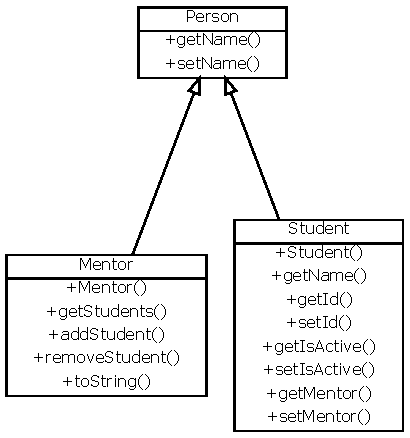
\includegraphics{Figures/Example1a1.pdf} 
\caption{UML class diagram of the Mentor-Student example - Level 1}
\label{fig:Example1a1}
\end{figure}

\subsection{School System: Transformations to Create Attributes}

Assuming that we have successfully performed the initial transformation on all the input files, at this point the input for the second transformation step are three Umple files.
We first analyze the variables (they are still variables even if they are inside an Umple class) to determine certain characteristics such as the following:

\begin{enumerate}
\item Is the field present in the parameters of the constructor?
\item Does the field possess a getter?
\item Does the field possess a setter?
\item Is the field's type, a primitive type?
\end{enumerate}

For instance, if we analyze the member variables in class Student, we obtain the results in Table \ref{table:analysisStudent}.

\begin{table}[ht]
\caption{Analysis of member variables of class Student}
\label{table:analysisStudent}
\centering
\begin{tabular}{l|cccc}
\toprule
\rowcolor[HTML]{BBDAFF}
\textbf{Member Variable} & \textbf{1}  & \textbf{2}   & \textbf{3}   & \textbf{4}    \\ \hline
id & Yes &  Yes &  Yes &  Yes \\ 
isActive &  No &  Yes &  Yes &  Yes \\ 
name &  Yes &  Yes &  No &  Yes \\ 
MAX\_PER\_GROUP &  No &  No &  No &  Yes \\ 
\hline
\end{tabular}
\end{table}

The results of this analysis allow us to generate Umple code with the required types and stereotypes. For example the stereotype `lazy' is added to `isActive' because it should not appear in the constructor, and the stereotype `immutable' is added to \textit{name} since there is no setter. The transformed Umple code after completion of this refactoring step (transformation 2a) is shown in Listing \ref{lst:studentUmple}. Note that this continues to generate a program that is semantically identical to the pre-transformation version.

\begin{lstlisting}[style=UmpleOut,caption=Student.ump,label=lst:studentUmple]
namespace university;

class Student { 
 isA Person;
 Integer id; 
 lazy Boolean isActive; 
 immutable name; 
 const Integer MAX_PER_GROUP = 10; 
 after getName {
  if (name == null) { 
   throw new RuntimeException("Error");
  }
 }
  public Mentor mentor; 
  public Mentor getMentor() { 
   return mentor; 
  }
  public void setMentor(Mentor mentor) { 
   this.mentor = mentor; 
  } 
}
\end{lstlisting}

% MG. Will be enhanced later, with titles in the boxes as in Ahmed's thesis.

The following gives details of Listing \ref{lst:studentUmple}:
\begin{itemize}
\item Line 5: Field id becomes an Umple attribute. Getter getId() and setter setId() are removed.


\item Line 6: Field isActive becomes an Umple attribute of Boolean type.  As the field is not required in the constructor, we mark it as `lazy' so the Umple compiler does not generate a constructor argument for this attribute. 

\item Line 7: Field name becomes an Umple attribute and is marked as `immutable'. Immutable attributes must be specified in the constructor, and no setter is provided. In this particular example, the input Java code (Listing \ref{lst:StudentJava}) does not contain code that sets this variable anywhere, therefore it is transformed into an immutable Umple attribute. 

\item Line 8: Field MAX\_PER\_GROUP becomes a constant (special type of Umple attribute). We have drawn this conclusion because of the field modifiers (e.g. static final) or because of the ALL\_CAPS convention. 

\item Line 9-13: As the getter for field name was custom in Listing \ref{lst:StudentJava}, we have adapted it so it conforms to the code that is generated by the Umple compiler. A code injection has been used for this purpose. In this case, the code will inject two lines to be executed before the getName() method returns.

\item Code in Lines 51-55 in Listing \ref{lst:StudentJava} is not touched by this transformation; The same exact code is found in the Umple file in Listing \ref{lst:studentUmple} (Lines 14-20).

\end{itemize}

In the same manner, we umplify the attributes of classes Mentor and Person.
The Umple code for class Mentor remains identical as in Listing \ref{lst:mentorUmple}, since we could not find any member variables in this class meeting the conditions to become an Umple attribute. On the other hand, the member variable `name' in class Mentor has been transformed into an attribute of String type. The resulting Umple code for class Person, after this transformation is shown below in Listing \ref{lst:personUmple}.

\begin{lstlisting}[style=UmpleOut,caption=Person.ump,label=lst:personUmple]
namespace university;
class Person {
 String name;
}
\end{lstlisting}

The visual representation of the Umple model at the end of this transformation step is shown in Figure \ref{fig:Example1a2}. At this point, we have gained knowledge about the hierarchical structure of the system and the attributes of each class. Associations are not shown in the diagram since they have not been yet reverse-engineered.

\begin{figure}[h]
\centering
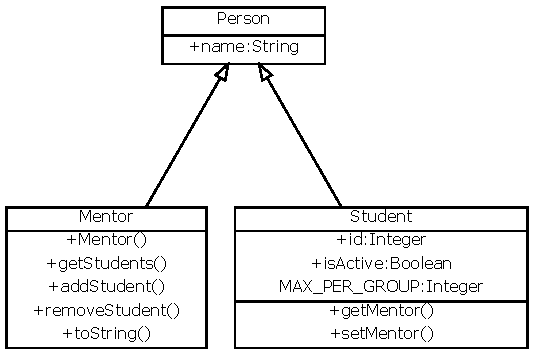
\includegraphics{Figures/Example1a2.pdf} 
\caption{UML class diagram of the Mentor-Student example - Level 2}
\label{fig:Example1a2}
\end{figure}

\subsection{School System: Transformations to Create Associations}

Assume again that the source code has already passed through the two first refactoring steps and the input at this point is the Umple code found in Listings \ref{lst:personUmple}, \ref{lst:mentorUmple} and \ref{lst:studentUmple}.

The resulting Umple code for class Mentor after completion of this refactoring step (transformation 2b) is shown below in Listing \ref{lst:mentorUmple2}. Line 2 contains the association derived from the Java code that can be read as: a mentor can have many students associated but a student can only be associated to at most one mentor. 

\begin{lstlisting}[style=UmpleOut,caption=Mentor.ump,label=lst:mentorUmple2]
namespace university;
class Mentor {
 0..1 -- 0..* Student; 
 
 public String toString() {
  return(
  (name==null ? " " : name) + " " +
   students.size()+ " students");
 }
}
\end{lstlisting}

\begin{lstlisting}[style=UmpleOut,caption=Student.ump,label=lst:studentUmple2]
namespace university;
class Student {
 Integer id; 
 lazy Boolean isActive; 
 immutable name; 
 const Integer MAX_PER_GROUP = 10; 
 
 after getName {
  if (name == null) { 
   throw new RuntimeException("Error");
  }
 }
}
\end{lstlisting}

The following particularities have been taken into consideration during the extraction of the association:

In class \textit{Mentor}:
\begin{enumerate}
\item The students variable in class Mentor is of a reference type and possesses a getter and a setter.
\item We inferred the multiplicity of the association end "0..*" by a) inspecting the cardinality of the member, and b) by analyzing the getter/setter of the member variable.
\item We inferred the navigability of the association "--" by inspecting the two classes involved. In this case, each class can access the linked objects of the other class.  The notation "-$>$" would otherwise have been used to represent a unidirectional association. 

\item The association end is optional-many because the member is not present as a parameter in the constructor (not required upon construction) of an instance of the class Mentor and because the member represents a collection of elements. 
\end{enumerate}

In class \textit{Student}:
\begin{enumerate}

\item The mentor in class Student is of a reference type and it possesses a getter and a setter.
\item We inferred the multiplicity of the association end "0..1" by inspecting the constructor of the class Student. It is optional-one because it is not required upon construction of class Student. 
\item Methods \textit{setMentor()} and \textit{getMentor()} are no longer needed in class Student and therefore removed.
\end{enumerate}

Consider again the previous example.  If we inject now the constructor of Listing \ref{lst:studentConstructor} into the Student class, the multiplicity for the association end would become "1" instead of "0..1". 

\begin{lstlisting}[style=java,caption=A new constructor added to Student class,label=lst:studentConstructor]
public Student(Mentor aMentor){
  mentor = aMentor;
}
\end{lstlisting}

Note that in the examples, the Java input made use of generics (templates using '$<>$' syntax) for the specification of a collection of elements. For those cases in which the type of the member variable cannot be directly inferred (in older Java code), we analyze the add/remove methods to determine the type of the element that is added to the collection. We will explore all possible detection mechanisms for associations in Chapter \ref{chap:detections}. Ultimately, each refactoring step should involve testing (running the test suites) to check that the program's semantics are preserved. 

The visual representation of the Umple model at the end of this transformation step is shown in Figure \ref{fig:Example1a3}. As a result,we have gained knowledge about the hierarchical structure of the system, attributes and associations of each class. 

\begin{figure}[h]
\centering
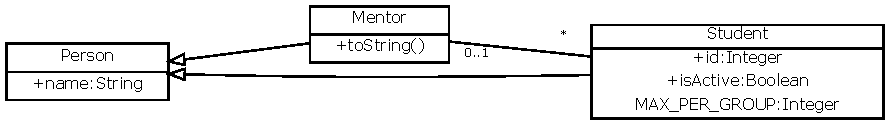
\includegraphics[width=0.90\textwidth]{Figures/Example1a3.pdf} 
\caption{UML class diagram of the Mentor-Student example - Level 3}
\label{fig:Example1a3}
\end{figure}

Finally, for this small system, the Umple code extracted (33 LOC) contains substantially fewer lines of code than the original system written in Java (77 LOC). Despite being a simple metric, the number of lines of code is a fair indicator of complexity \cite{LOCMetric}. 

\section{ATM System - Manual Umplification Example}

In this section, we will manually umplify a second, moderately-sized Java system comprised of:

\begin{itemize}
 \item 24 files, 2470 Lines of Code.
 \item Two top packages \textit{atm} and \textit{banking}.
	\begin{itemize}
	 \item atm: ATM, Session
	 \item atm.physical: CardReader, CashDispenser, CustomerConsole, EnvelopeAcceptor, Log, NetworkToBank, OperatorPanel, ReceiptPrinter
	 \item atm.transaction: Transaction, Withdrawal, Deposit, Transfer, Inquiry
	 \item banking: AccountInformation, Balances, Card, Message, Money, Receipt , Status.
	\end{itemize}
 \item Two `top-level' classes: ATMMain and ATMApplet allowing the system to be run as an application or as an applet.
\end{itemize}

The original Java source code has been taken from \cite{atmsystem}. Although this can be considered as a small application, by going through the source code of the ATM program, it is not easy to understand how the classes are organized, how they interact with each other and how the responsibilities are distributed among the classes. A programmer aiming to use, document or extend this ATM application may want to know the impact of a change by looking at the dependencies, generalizations and associations connecting the entities or to obtain a high level view of the system for program understanding. The reader can take any versions of the code, at each step of umplification (obtained from \cite{UmplificationBasicExampleURL}), and paste it into UmpleOnline \cite{UmpleOnline} or our Eclipse-based Umple environment. 

% Abpve. Really you can paste the full system with all its classes into UmpleOnline? Maybe it can handle such a large body of code. I am a little surprised.

In the following sub-sections, we present the transformation details for the classes in package `atm.banking' and the main program class for the system `ATMMain.java'. Note that the comments have been ignored and code in some methods have been omitted from this thesis to save space.  Listings \ref{lst:CardJava} - \ref{lst:ATMMainJava} present each of the classes in this package, the input code. The Umple code resulting from each step will be shown as well as the UML class diagram (visual representation of the model). 

\noindent\begin{minipage}{.45\textwidth}
\begin{lstlisting}[style=java,caption=Card.java,label=lst:CardJava]{Name}
package banking;

public class Card
{
 private int number;
    
 public Card(int number)
 {
  this.number = number;
 }
    
 public int getNumber()
 {
  return number;
 }   
}
\end{lstlisting}
\end{minipage}\hfill
\begin{minipage}{.45\textwidth}
\begin{lstlisting}[style=java,caption=AccountInfo.java,label=lst:AccountInformation]{Name1}
public class AccountInformation
{
 public static final String [] ACCOUNT_NAMES =
    { "Checking", "Savings", "Money Market" };
         
 public static final String [] ACCOUNT_ABBREVIATIONS =
    { "CHKG", "SVGS", "MMKT" };
}    
\end{lstlisting}
\end{minipage}


\noindent\begin{minipage}{.45\textwidth}
\begin{lstlisting}[style=java,caption=Status.java,label=lst:Status]{Name}
package banking;

public abstract class Status
{
 public String toString()
 {
  if (isSuccess())
   return "SUCCESS";
  else if (isInvalidPIN())
   return "INVALID PIN";
  else
   return "FAILURE " + getMessage();
 }
    
 public abstract boolean isSuccess();
 public abstract boolean isInvalidPIN();
 public abstract String getMessage();
}
\end{lstlisting}
\end{minipage}\hfill
\begin{minipage}{.45\textwidth}
\begin{lstlisting}[style=java,caption=Receipt.java,label=lst:Receipt]{Name1}
package banking;

import atm.ATM;
import atm.transaction.Transaction;
import java.util.Date;
import java.util.Enumeration;

public abstract class Receipt
{

 private String [] headingPortion;
 protected String [] detailsPortion;
 private String [] balancesPortion;  
    
 protected Receipt(ATM atm, Card card, Transaction transaction, Balances   balances)
 {        
  // Code omitted
 }
     
 public Enumeration getLines()
 {
  // Code omitted
 }
}
\end{lstlisting}
\end{minipage}

\noindent\begin{minipage}{.45\textwidth}
\begin{lstlisting}[style=java,caption=Balances.java,label=lst:Balances]{Name}
package banking;

public class Balances
{
 private Money total;
 private Money available;
    
 public Balances(){}
    
 public void setBalances(Money total, Money available)
 {
   this.total = total;
   this.available = available;
 }
    
 public Money getTotal()
 {
  return total;
 }
    
 public Money getAvailable()
 {
  return available;
  }
}
\end{lstlisting}
\end{minipage}\hfill
\begin{minipage}{.45\textwidth}
\begin{lstlisting}[style=java,caption=Money.java,label=lst:Money]{Name1}
package banking;

public class Money
{ 
 private long cents; 
   
 public Money(int dollars)
 {
  this(dollars, 0);
 }
   
 public Money(int dollars, int cents)
 {
  this.cents = 100L * dollars + cents;
 }
    
 public Money(Money toCopy)
 {
  this.cents = toCopy.cents;
 }
    
 public String toString()
 {
  return "$" + cents/100 + 
  (cents %100 >= 10  ? "." + cents % 100 : ".0" + cents % 100);
 }
    
 public void add(Money amountToAdd)
 {
  this.cents += amountToAdd.cents;
 }

 public void subtract(Money amountToSubtract)
 {
  this.cents -= amountToSubtract.cents;
 }

 public boolean lessEqual(Money compareTo)
 {
  return this.cents <= compareTo.cents;
 }
}
\end{lstlisting}
\end{minipage}

\subsection{ATM System: Initial Transformation}

As in the school example described earlier, we start by creating the .ump files, one Umple file per input class. A total of 24 Umple files (7 for the package `atm.banking') are created as result of this initial transformation.

The dependency, package and generalization notations are changed to their respective Umple notations.

For instance, the Java code (in file ATMMain.java) shown in Listing  \ref{lst:ATMMainJava} would result in the Umple implementation shown in Listing  \ref{lst:ATMMainUmple} (in file ATMMain.ump). Only the code transformed has been shown in Listings \ref{lst:ATMMainJava} -- \ref{lst:ATMMainUmple}. `The rest of the code' corresponds to the code that has not been touched during the transformation. 

\noindent\begin{minipage}{.45\textwidth}
\begin{lstlisting}[style=java,caption=ATMMain.java,label=lst:ATMMainJava]{Name}
import java.awt.*;
import java.awt.event.*;
import atm.ATM;
import simulation.Simulation;

// Main program  
public class ATMMain
{
   // The rest of the code
}
\end{lstlisting}
\end{minipage}\hfill
\begin{minipage}{.45\textwidth}
\begin{lstlisting}[style=UmpleIn,caption=ATMMain.ump,label=lst:ATMMainUmple]{Name1}
// Main program  
class ATMMain
{
  depend simulation.Simulation;
  depend atm.ATM;
  depend java.awt.event.*;
  depend java.awt.*;
  // The rest of the code
}
\end{lstlisting}
\end{minipage}

At the end of this transformation step, the visual representation of the umplified model is shown in Figure \ref{fig:atmBanking1}. At this point, we have gained knowledge about the hierarchical structure of the system. Attributes and associations are not shown in the diagram since they have not been yet reverse-engineered (umplified).

\subsection{ATM System: Transformations to Create Attributes}

Once again, the input for the second transformation step is the set of Umple files produced in the previous step. The next step then recovers the attributes. The visual representation of the umplified model is shown in Figure \ref{fig:atmBanking2}.

\begin{figure}[!ht]
\centering
\begin{minipage}[b]{0.47\linewidth}
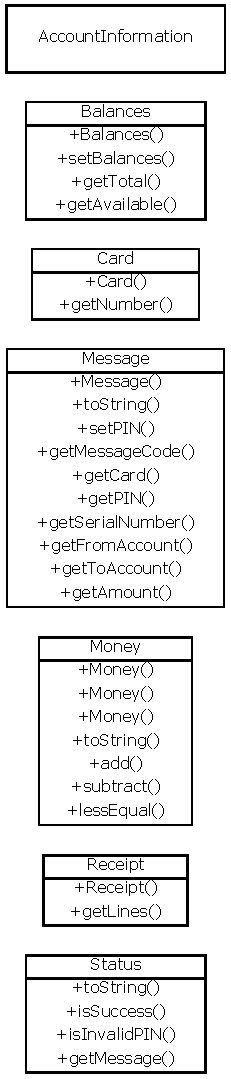
\includegraphics{Figures/Example2a1.pdf}
\caption{UML class diagram of the ATM example - Level 1}
\label{fig:atmBanking1}
\end{minipage}
\quad
\begin{minipage}[b]{0.47\linewidth}
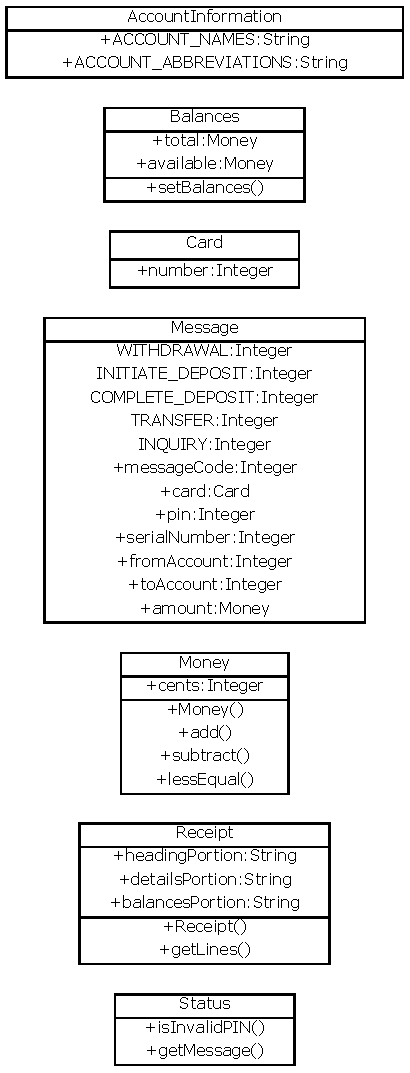
\includegraphics{Figures/Example2a2.pdf}
\caption{UML class diagram of the ATM example - Level 2}
\label{fig:atmBanking2}
\end{minipage}
\end{figure}

% better if these figures list the classes horizontally. There is a lot of wasted space on these two pages.
% MG. Fixed. Two figures in one page (see above).
The following is a summary of the various considerations that were taken into account to perform this transformation step:

\begin{itemize}
\item Fields (possessing the characteristics described before) were transformed into Umple attributes. 

\item Constructors were removed from the resulting code. They are not required since Umple generates constructors and in this case they conform to those generated by Umple. 

\item Mutator and accessor methods were removed from the resulting code. Once again, the Umple compiler will regenerate these. 

\item \textit{Status} class was transformed into an \textit{abstract} Umple class. 

\item In class \textit{Balance}, Money is transformed into an attribute since this class contains only fields of primitive data type. Refer to subsection \ref{subsection:overview} for more details.
\end{itemize}

Since there was not a proper set of test cases available, we run a simulation of a series of transactions to verify that the program's semantics were preserved. In fact, the simulation was performed following the  `startup', `shutdown', `transaction' and `session', `withdrawal', `deposit' and `transfer' use cases as described in the documentation of the ATM system \cite{atmsystem}.


\subsection{ATM System: Transformations to Create Associations}

Once the code/model has  passed through the two first refactoring steps, we perform the transformation step aiming to recover associations from the input classes.

The result (`atm.banking') produced is shown in Figure \ref{fig:atmBanking3}. For conciseness, only classes with associations are shown as part of this class diagram. As mentioned before, the source code of the ATM system can be found at \cite{atmsystem}.
%LAST - see above

For instance, the following is a summary of the various considerations that were taken into account to perform this transformation step on classes \textit{ATM} and \textit{Session}:

\begin{itemize}
\item The instance variable `atm' in class \textit{Session} becomes one end of an association. 
Note that the variable is present in the (unique) constructor of class Session. The multiplicity of this association end is therefore `0..1'.

\item We look in class ATM for any instance variable of type Session. Since the instance variable is a collection of Session instances, the variable `sessions' becomes the other association end. Note that the variable is not present as one of the constructor arguments. Multiplicity of this association end is therefore `*'.

\item The rolenames of the associations ends are inferred from the variable names.

\item Constructors in both classes are removed.

\item Method `getATM()' is removed from the class \textit{Session}.

\item Method `getCSession(int sessionID)' is removed from the class \textit{ATM} as Umple will generate a method with the following signature `public Session getSession(int index)'.

\item Association in Umple notation becomes:  `0..1 ATM --  * Session;'.
\end{itemize}

\begin{figure}[!ht]
\centering
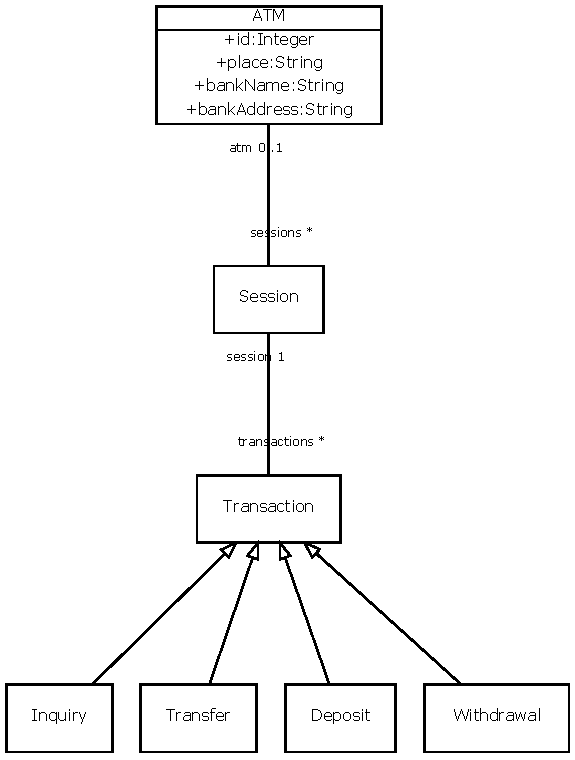
\includegraphics{Figures/Example2a3.pdf} 
\caption{UML class diagram of the ATM example - Level 3}
\label{fig:atmBanking3}
\end{figure}

As in our previous step, the simulation was run to ensure that the program's semantics were still preserved.

% Note the lines-of-code differenced  (the number of lines of code).

\section{Summary}

Umplification is a process for converting a base language program into an Umple program, involving a set of transformation steps. Umplification responds to several needs: The first concerns models that become obsolete very quickly; umplification ensures that from this point on the model can be maintained with the code as it is part of the code. Another need addressed is the desire to simplify existing systems by avoiding the need to write boilerplate code.

In this chapter, we have discussed some transformation steps and demonstrated performing umplification manually. In the next chapter, we will present the mapping rules derived from each of the transformation steps. These transformation rules will be necessary to automate our reverse engineering process. Implementation of the mapping rules is then presented in Section \ref{chap:tool}.
 % Reverse Engineering

\lhead{\emph{\leftmark}}  

\chapter{Detection Mechanisms for UML/Umple Constructs}
\label{chap:detections}

In this chapter, we will present the different mechanisms to detect UML/Umple attributes, associations and state machines from source code written in an object-oriented programming language. We started to build our detection rules based on the following:

\begin{enumerate}

\item Documented implementations of attributes and associations in high-level programming languages mentioned in the literature. In particular, we have considered research that discusses how to generate code from these modeling concepts (forward engineering).

\item Documented techniques in the literature for discovering  modeling constructs in object-oriented source code (reverse engineering).

\item Our own analysis of open source systems written in object-oriented programming languages.

\end{enumerate}

To present the set of transformation rules derived from our analysis, we  employ a semi-formal notation. The rules define the transformation from input to output. These transformations rules can be described using a metamodel-based language or grammar-based language. Both types of descriptions allow us to specify mappings between source and target models in the form of conditions (patterns) and conversions (replacements) executed from input to output when those conditions hold. As the intent of our work is to transform object-oriented  language programs into Umple programs, we  employ a metamodel-based approach to better express the input/output relationships. The metamodel-based language will be enhanced with OCL \cite{WarmerOCL2003} expressions. 
% create table in chapter 5, showing m2t and m2m requirements in terms of Model source code
% M2M: UmpleModel, JavaModel
% M2T: JavaModel, UmpleCode
% T2T: Java code, Umple Code

\section{A Notation for Transformation Rules}
\label{sec:2ModelTransformation}

Transformation rules presented in this chapter contain the following information:

\begin{enumerate}

\item A name for each transformation rule used for reference purposes.

\item The source language reference.

\item Constants used in the generation of the target.

\item Helper methods used in the extraction of information from target or input models.

\item A set of named source language model elements from the source language metamodel that we call B.

\item A set of named target language model elements from the target language metamodel that we call U.

\item The source language conditions: invariants that state the conditions that must hold in the source model for this transformation to be applied.

\item The target language conditions: invariants that state the conditions that must hold in the target model for this transformation to be applied.

\end{enumerate}

% It would be better in this template if the keyword 'conditions' and 'mappings' would be in blue, just like 'in' and 'out'
% MG Fixed

Listing \ref{lst:templateTransform} presents a template definition for the transformations rules.

\begin{lstlisting}[style=mine,caption=Template definition for transformation rules,label=lst:templateTransform]
Transformation Name  (InputModel, OutputModel){
 order n
 params
 	...
 in
   sourceElement: ...
 out
   targetElement: ...
 in-out conditions
 	...
 mappings
    sourceElement.propertyA -> targetElement.propertyA;
    sourceElement.propertyB -> targetElement.propertyB;
}
\end{lstlisting}

The various parts of a transformation rule have their own  specific notation:

\begin{itemize}

\item Line 1. Every transformation possesses a name. The source and target languages are referenced by stating both language names after the transformation name.

\item Line 2. The order of application of the rule is determined by the integer number following the keyword \textit{order}. Rules with lower order numbers are executed first. Order of application of the rules does not matter when two or more rules possess the same order number. 

\item Line 3. Local and global variables to be used in the transformation rule are specified following the keyword \textit{params}.

\item Lines 5 and 7. The source model and target elements are written as variable declarations following the keywords \textit{in} and \textit{out} respectively.

\item Line 9. The conditions that must hold on the source and target model elements are specified following the keywords \textit{in-out conditions}. The mappings are performed only if all conditions specified are true. Conditions are specified using OCL syntax. 

\item Line 11. The mapping rules come after the keyword \textit{mappings}. The symbol -\textgreater \newline is used as an infix operator with two operands. The symbol specifies a transformation of the left hand side operand to the right side operand (rules are unidirectional).
\end{itemize}

We will now introduce the transformation rules for each of the transformation steps presented in Chapter \ref{chap:core}.
The set of rules for each transformation case constitutes a transformation case definition. Rules in the set are to be executed in sequence.

\section{Transformation Rules for the Initial Transformation Step}

Transformations rules for this step are straightforward and aim at transforming the package declaration, namespace declarations, import declaration and the generalization notation into the corresponding Umple notation. 

The mapping rule in Listing \ref{lst:4.1.1} specifies the transformation of a Class into an Umple class using the language defined in the previous section. A type declaration in the base language model represents an object-oriented type (i.e., a class, interface, struct, etc). The only required condition in the rule shown in Listing \ref{lst:4.1.1} (Line 7) is that the \textit{typeDeclaration} must declare a class and not an interface or abstract class. A very similar rule is then required for the transformation of a \textit{typeDeclaration} into an Umple Interface. The relationship between the source model, the target model and the mapping rule (in blue background) are illustrated in Figure \ref{fig:4.1.1}.
Transformation rules defined in a general but formal language can then be adapted to specific languages such as Java or C++. For instance, the name of a typeDeclaration if the input language is Java can be extracted using the \textit{getName().getFullyQualifiedName()} call sequence. Actual implementation of the mapping rules will be presented in Chapter \ref{chap:tool}. For our first example, we show the BNF grammar for a type declaration in Java and an Umple class declaration in Listings \ref{lst:javaGrammar1} and \ref{lst:umpleGrammar2} respectively. It must be pointed out that the transformation rule can be understood either by looking at the metamodel or the grammar of input/output models. 

% The following Listing is totally mixed up with the subsequent figure in the tool, but when I export a pdf it looks OK. Very strange.
% MG. Strange, I see the same problem. PDF will be fine however.

% Also, you are using tabs, which Latex does not process properly in listings. You need to use two spaces instead of tabs. I have made this change in this case, but make the change elsewhere and watch out in other code.
% Fixed MG.

% Readers will be confused as to the detailed sublanguages (e.g. the reference to isInterface(), ::TypeDeclariation, .name and so on. How are you going to define these? I know you say this is 'informal' (actually I changed it to 'semiformal' which is the correct term), but nonetheless it should be understandable. Are you referring to JDT contstructs? If so then there is the problem that you have not introduced JDT yet. Perhaps the solution is to put much of Chapter 5 before this (discussing how you tried ATL, TXL and then briefly xDT), then have this chapter, which can now refer to JDT, and finally discuss the implification in another separate chapter. There would end up being one more chapter than there is now.
% But there may be another way to make this all make sense, such as defining the semi-formal language in a simple way here.
% MG Fixed by using a more abstract way of presenting the language. 

\begin{lstlisting}[style=mine,caption=Grammar for Java types,label=lst:javaGrammar1]
TypeDeclaration:
                ClassDeclaration
                InterfaceDeclaration
 ClassDeclaration:
      [ Javadoc ] { Modifier } class Name
                        [ extends Type]
                        [ implements Type { , Type } ]
                        { { ClassBodyDeclaration | ; } }
 InterfaceDeclaration:
      [ Javadoc ] { Modifier } interface Identifier
                        [ extends Type { , Type } ]
                        { { InterfaceBodyDeclaration | ; } }
\end{lstlisting}

\begin{lstlisting}[style=mine,caption=Grammar for Umple classes,label=lst:umpleGrammar2]
 umpleClass : class Name { [[classContent]]* }
\end{lstlisting}

\begin{lstlisting}[style=mine,caption=Rule BaseTypeToUmpleClass,label=lst:4.1.1]
Transformation BaseTypeToUmpleClass (BaseLanguageMetamodel, UmpleMetamodel){ 
 in
   typeDeclaration : BaseLanguageModel::TypeDeclaration;
 out
   UmpleClass: UmpleMetamodel::UmpleClass;
 in conditions
   typeDeclaration.oclIsTypeOf(ClassDeclaration);   
 mappings
   typeDeclaration.name -> UmpleClass.name;
}
\end{lstlisting}

\begin{figure}[h]
\centering
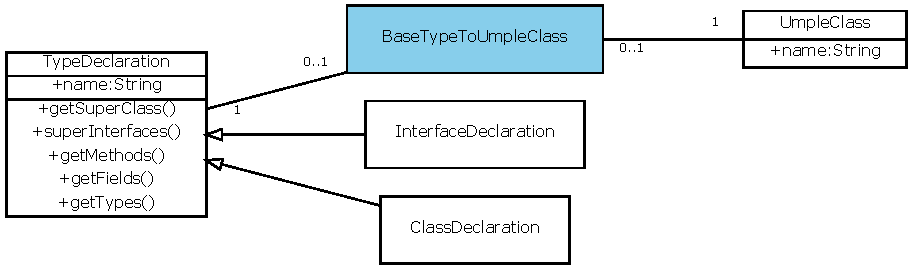
\includegraphics[width=0.99\textwidth]{Figures/ch4InitialMapping.pdf}
\caption{Input-output relationships for rule BaseTypeToUmpleClass}
\label{fig:4.1.1}
\end{figure}

Similarly, rule  \textit{ImportToUmpleDepend} in Listing \ref{lst:4.1.2} specifies the transformation of an import declaration into a depend declaration. Import directives in object-oriented languages are used to incorporate information from a type library. 

\begin{lstlisting}[style=mine,caption=Rule JavaImportToUmpleDepend,label=lst:4.1.2]
Transformation ImportToUmpleDepend (BaseLanguageMetamodel, UmpleMetamodel){ 
 in
   importDeclaration : BaseLanguageModel::ImportDeclaration;
 out
   depend: UmpleMetamodel::Depend;
 in-out conditions
	none
 mappings
   importDeclaration.name -> depend.name;
   fieldDeclaration.importDeclaration -> UmpleClass.depend;
}
\end{lstlisting}

Rule \textit{PackageToUmpleNamespace} in Listing \ref{lst:4.1.3} specifies the transformation of a package declaration into a namespace declaration in Umple. Package declarations in object-oriented languages are used to organize and group classes.

\begin{lstlisting}[style=mine,caption=Rule PackageToUmpleNamespace,label=lst:4.1.3]
Transformation PackageToUmpleNamespace (BaseLanguageMetamodel, UmpleMetamodel){ 
 in
   packageDeclaration : BaseLanguageModel::PackageDeclaration;
 out
   UmpleClass: UmpleMetamodel::UmpleClass;
 in-out conditions
    none
 mappings
   packageDeclaration.name -> UmpleClass.namespace;
}
\end{lstlisting}

Furthermore, the generalization in the base language notation is transformed into the Umple notation \textit{isA} as shown in Listing \ref{lst:4.1.5}.

\begin{lstlisting}[style=mine,caption=Rule GeneralizationToUmpleIsA,label=lst:4.1.5]
Transformation GeneralizationToUmpleIsA (BaseLanguageMetamodel, UmpleMetamodel){ 
 in
   typeDeclaration : BaseLanguageModel::TypeDeclaration;
 out
   UmpleClass: UmpleMetamodel::UmpleClass;
 in conditions
   typeDeclaration.oclIsTypeOf(ClassDeclaration);   
 mappings
   typeDeclaration.superInterfaceTypes -> UmpleClass.parentInterfaces;
   typeDeclaration.superClassType -> UmpleClass.extendsClass;
}
\end{lstlisting}

At this transformation step, we do not attempt to transform any variable into an Umple attribute, association end or state machine. As a result the field declarations and related method declarations are simply appended to the body of the Umple class; some of these will be transformed later. The rule \textit{ClassBodyToUmpleClassExtracode} in Listing \ref{lst:4.1.4} performs the desired operation. We employ the OCL feature \textit{iterate} to traverse the collection of methods and fields belonging to the field declaration. 

\begin{lstlisting}[style=mine,caption=Rule ClassBodyToUmpleClassExtracode,label=lst:4.1.4]
Transformation ClassBodyToUmpleClassExtracode (BaseLanguageMetamodel, UmpleMetamodel){ 
 in
   fieldDeclaration : BaseLanguageModel::FieldDeclaration;
   methodDeclaration : BaseLanguageModel::MethodDeclaration;
   typeDeclaration : BaseLanguageModel::TypeDeclaration;
 out
   UmpleClass: UmpleMetamodel::UmpleClass;
 in conditions
   typeDeclaration.oclIsTypeOf(ClassDeclaration);   
 mappings
   typeDeclaration->iterate( f: FieldDeclaration | 
     fieldDeclaration.toString -> UmpleClass.extraCode);
   methodDeclaration->iterate( f: FieldDeclaration | 
     fieldDeclaration.toString -> UmpleClass.extraCode);
}
\end{lstlisting}

Rules aiming at transforming type declarations into Umple interfaces are very similar to those presented above except that now the `in-out' condition becomes: 
\newline
`\textit{oclIsTypeOf(InterfaceDeclaration)}'.

Finally, enumerations are umplified into Umple `enums'. An \textit{enum} in Umple is a state machine that has events.

\section{Member Variables Analysis}
Member variables can represent not only attributes, but also associations, state machine variables, and internal data such as counters, caching, or sharing of local data. In this section, we analyze the characteristics of member variables and present the mapping rules guiding the transformation of
these member variables into attributes or associations variables. Furthermore, we analyze the different patterns supported by existing reverse engineering tools when it comes to the detection of these UML/Umple constructs. 

\subsection{Transformations Rules to Create Attributes}
%FINAL CHANGE START
The first part of our analysis, as stated at the beginning of this Chapter, consists of analyzing how real projects implement attributes. In previous work done by co-researchers \cite{UmpleAttributes} seven projects picked randomly from open source repositories were studied. The seven projects included: from GoogleCode: fizzbuzz, ExcelLibrary, ndependencyinjection and Java Bug Reporting Tool; from SourceForge: jEdit and Freemaker; and from Freecode (formerly Freshmeat): Java Financial Library.
Refer to Table \ref{table:umplifiedSystems} for details about the systems. 
%LAST added reference to table in chapter 6
%FINAL CHANGE END

From these projects, we identified 1831 member variables in the 469 classes analyzed. From the member variables found, 1211 were instance variables and 620 were class (static) variables. The results of this study showed that:

\begin{itemize}
\item 27\% of the instance variables were of a number type. This includes primitive integers, unsigned and signed numbers.
\item 14\% of the instance variables were of a string type. 
\item 10\% of the instance variables were of Boolean type.
\item 2\% of the instance variables were of Date and Double type.
\item 47\% of the instance variables were of a different data type (reference type).
\end{itemize}

As discussed in Chapter \ref{chap:core} and presented in the study done by co-researchers \cite{UmpleAttributes}, the type of an (candidate) attribute is either a simple data type such as the types in Table \ref{table:attributes2} or a class that contains itself only instance variables of primitive type. The latter case is illustrated through Listings \ref{lst:PersonCandidateAttr}-\ref{lst:AddressCandidateAttr}. In the example, the class \textit{Address} (a reference type) contains only instance variables of primitive type and therefore is more likely an attribute. 

\begin{table}
\caption{Umple primitive data types}
\label{table:attributes2}
\centering
    \begin{tabular}{ll}
		\toprule
		\rowcolor[HTML]{BBDAFF}
        \textbf{Type}      & \textbf{Description}                               \\ 
        \hline
        Integer   & Includes signed and unsigned integers.    \\ 
        String    & All string and string builder types       \\ 
        Boolean   & true/false types                          \\ 
        Double    & All decimal object types                  \\ 
        Date/Time & All date, time and calendar object types. \\
        \hline
    \end{tabular}
\end{table}

\noindent\begin{minipage}{.45\textwidth}
\begin{lstlisting}[style=java,caption=Person.java,label=lst:PersonCandidateAttr]{Name}
public class Person {
 private Address address;
 // ... Other parts omitted
}
\end{lstlisting}
\end{minipage}\hfill
\begin{minipage}{.45\textwidth}
\begin{lstlisting}[style=java,caption=Address.java,label=lst:AddressCandidateAttr]{Name}
public class Person {
 // ... Other parts omitted
 // Getters, setters and constructors omitted
 private String postalCode;
 private int streetNumber;
 private String streetName;
 private int apptNumber;
}
\end{lstlisting}
\end{minipage}

Candidate attributes, those instance variables possessing the characteristics mentioned above, are further analyzed. The instance variables were analyzed for their presence in constructors and in and get/set methods. This is a key fact that helped us determine whether the member variable can indeed become an Umple attribute. Table \ref{table:attributesAnalysis} presents the results for this part of the study.
Those instance variables with high and medium probability are definitely attributes. The instance variables with a low or very low probability of being attributes are not transformed for now. 

\begin{table}[h]
\caption{Analyzing instance variables for presence in the constructor and getter/setters}
\label{table:attributesAnalysis}
\centering
\begin{tabular}{@{}cccc@{}}
\toprule
\rowcolor[HTML]{BBDAFF}
\multicolumn{1}{c}{\cellcolor[HTML]{BBDAFF}\textbf{Constructor}} & \multicolumn{1}{c}{\cellcolor[HTML]{BBDAFF}\textbf{Setter}} & \multicolumn{1}{c}{\cellcolor[HTML]{BBDAFF}\textbf{Getter}} & \multicolumn{1}{c}{\cellcolor[HTML]{BBDAFF}\begin{tabular}[c]{@{}c@{}}\textbf{Attribute}\\ \textbf{(Probability})\end{tabular}} \\ \midrule
Yes                                                     & Yes                                                & Yes                                                & High                                                                                                          \\
Yes                                                     & Yes                                                & No                                                 & Low                                                                                                           \\
Yes                                                     & No                                                 & Yes                                                & High                                                                                                          \\
Yes                                                     & No                                                 & No                                                 & Low                                                                                                           \\
No                                                      & Yes                                                & Yes                                                & High                                                                                                          \\
No                                                      & Yes                                                & No                                                 & Low                                                                                                           \\
No                                                      & No                                                 & Yes                                                & Medium                                                                                                        \\
No                                                      & No                                                 & No                                                 & Very Low                                                                                                      \\ \bottomrule
\end{tabular}
\end{table}

As presented in Chapter \ref{chap:background}, attributes can be categorized into 4 main categories: \textit{lazy}, fully editable, derived or immutable. By analyzing the presence of the variable in the constructor, getter and setter we can determine to which of the categories the extracted attributes belongs to. Table \ref{table:constructorFrequency} presents the different categories of attributes and whether or not they are required as arguments in the constructor, getter and setters. Lazy attributes for instance are those with postponed initialization (third line in Table \ref{table:constructorFrequency}). Therefore, when the member variable 
\begin{enumerate*}
  \item has a \textit{Get} method,
  \item has a \textit{Set} method and
  \item is not one of arguments of the constructor 
\end{enumerate*}, it is matched (converted) into a lazy Umple attribute. 

\begin{table}
\caption{Type of attribute based on their presence in constructor and access method patterns}
\label{table:constructorFrequency}
\centering
\begin{tabular}{llll}
\toprule
\rowcolor[HTML]{BBDAFF}
\textbf{Type}   & \textbf{Contructor}    & \textbf{Setter}       &  \textbf{Getter} \\ 
\hline
 Fully editable & Yes & Yes & Yes \\
  Immutable & Yes & No & Yes \\
   Lazy & No & Yes & Yes \\
    Derived & No & No & Yes \\
\hline
\end{tabular}
\end{table}

Results of the first part of the analysis on the seven open-source projects can be found at:
\url{https://github.com/mgarzon/experiments/mgarzon/thesis/CH4Detection}.

The second part of our analysis of attributes consisted of reviewing how other reverse engineering tools 
recover attributes from source code. Reverse engineering tools in Table \ref{table:toolsReverse} were employed to recover attributes from (Java) source code. Since all the tools mentioned above generate UML models from source code (and not Umple models) we are not concerned here about the `lazyness' or `immutability' characteristics of the attributes. In fact, we are only concerned about the following:

\begin{table}[h]
\caption{Reverse-engineering tools evaluated}
\label{table:toolsReverse}
\centering
\begin{tabular}{lll}
\toprule
\rowcolor[HTML]{BBDAFF}
\textbf{Tool}   & \textbf{Version}  & \textbf{Type}\\ 
\hline
 ArgoUML \cite{ArgoUML} & 0.32.2 & Open-source \\
 Intellij IDEA \cite{IdeaTool} & 14.1 & Commercial \\
 Visual Paradigm \cite{VisualParadigm} & 12.0 & Commercial  \\
 Rational Rose Modeler  \cite{ROSE} & 7.1 & Commercial\\
 Fujaba \cite{Fujaba} & (Reclipse) 1.0 & Research\\
 Ptidej \cite{ptidejTool} & 5.8 & Research\\
\hline
\end{tabular}
\end{table}

\begin{enumerate}
\item Is the tool able to correctly recover the type of the attribute?

\item Is the tool able to distinguish cases in which the member variable is of a reference type but that type contains itself only variables of primitive type? It is a correct recovery if the member variable is extracted as an attribute and not as an association (one-to-one)?

\item Is the tool able to distinguish a `local variable' from a real attribute by analyzing the presence of an accessor/mutator in the source code?  It is a correct recovery if only member variables possessing a getter are recovered as attributes. 

\item Is the tool able to deal with all the many different ways of coding an accessor/mutator? `N/A' in this context means that the tool does not analyze constructors, mutators or accessors when recovering attributes. 

\item Is the tool able to distinguish between one (0..1 or 1) and many (*) based on the attribute type? It is a correct recovery if list structures and object types with a plural noun were identified as \textit{many}, all other structures should be identified as \textit{one}. An example of an attribute with  \textit{many} multiplicity is `List\textless String \textgreater ids'.

\item Is the tool able to recover class level attributes (i.e. static)?
\end{enumerate}

Table \ref{table:analyzeAttributesSecondPart} presents the results.

\begin{table}[h]
\caption{Analysis of reverse-engineering tools for the recovery of attributes}
\label{table:analyzeAttributesSecondPart}
\centering
\begin{tabular}{lllllll}
\toprule
\rowcolor[HTML]{BBDAFF}
\textbf{Tool}   & \textbf{1}    & \textbf{2}   &  \textbf{3}   &  \textbf{4} &  \textbf{5}  &  \textbf{6} \\ 
\hline
ArgoUML & Yes & No & No & N/A & No & Yes\\ 
IDEA & Yes & No & No & No & No  & Yes\\ 
Visual Paradigm & Yes & No & Yes & No & No & Yes \\ 
Rational Rose & Yes & Yes & No & No & Yes & Yes\\ 
Fujaba & Yes & Yes & No & Yes & Yes & Yes\\ 
Ptidej & Yes & Yes & No & N/A & Yes & Yes\\ 
\hline
\end{tabular}
\end{table}

By analyzing existing projects and assessing how reverse engineering tools recover attributes, we were able to align our detection mechanisms (mapping rules) with the observed trends, and ensure our tool fills in the gaps that other tools leave.

The mapping rules obtained from our analysis are presented next.

\begin{lstlisting}[style=mine,caption=Case 1 - Variable has a getter ,label=lst:attrCase1]
Transformation FieldToUmpleBasicAttribute (BaseLanguageMetamodel, UmpleMetamodel){ 
 in
   fieldDecl : BaseLanguageModel::FieldDeclaration;
 out
   attr: UmpleMetamodel::Attribute;
 in-out conditions
 	fieldDecl.type.oclIsTypeOf(PrimitiveType) 
 	   OR fieldDecl.type.oclIsTypeOf(ComplexType) ;
 	hasAGetter(fieldDecl);
 mappings
    fieldDecl.name -> attr.name;
    fieldDecl.type -> attr.type;
}
\end{lstlisting}

\begin{lstlisting}[style=mine,caption=Is a fully editable attribute,label=lst:attrCase2]
Transformation FieldToUmpleFullAttribute (BaseLanguageMetamodel, UmpleMetamodel){ 
 in
   fieldDecl : BaseLanguageModel::FieldDeclaration;
 out
   attr: UmpleMetamodel::Attribute;
 in-out conditions
 	fieldDecl.type.oclIsTypeOf(PrimitiveType)
 	    | fieldDecl.type.oclIsTypeOf(ComplexType);
 	hasAGetter(fieldDecl);
 	hasASetter(fieldDecl);
 	hasAConstructor(fieldDecl);
 mappings
    fieldDecl.name -> attr.name;
    fieldDecl.type -> attr.type;
}
\end{lstlisting}

\begin{lstlisting}[style=mine,caption=Is an immutable attribute,label=lst:attrCase3]
Transformation FieldToUmpleImmutableAttribute (BaseLanguageMetamodel, UmpleMetamodel){ 
 in
   fieldDecl : BaseLanguageModel::FieldDeclaration;
 out
   attr: UmpleMetamodel::Attribute;
 in-out conditions
 	fieldDecl.type.oclIsTypeOf(PrimitiveType)
 	 | fieldDecl.type.oclIsTypeOf(ComplexType);
 	hasAGetter(fieldDecl);
 	hasASetter(fieldDecl)==false;
 	hasAConstructor(fieldDecl);
 mappings
    fieldDecl.name -> attr.name;
    fieldDecl.type -> attr.type;
}
\end{lstlisting}

\begin{lstlisting}[style=mine,caption=Is a lazy attribute,label=lst:attrCase4]
Transformation FieldToUmpleLazyAttribute (BaseLanguageMetamodel, UmpleMetamodel){ 
 in
   fieldDecl : BaseLanguageModel::FieldDeclaration;
 out
   attr: UmpleMetamodel::Attribute;
 in-out conditions
 	fieldDecl.type.oclIsTypeOf(PrimitiveType)
 	   | fieldDecl.type.oclIsTypeOf(ComplexType);
 	hasAGetter(fieldDecl);
 	hasASetter(fieldDecl);
 	hasAConstructor(fieldDecl)==false;
 mappings
    fieldDecl.name -> attr.name;
    fieldDecl.type -> attr.type;
}
\end{lstlisting}

These high-level rules are implemented in the Drools language and presented in Chapter \ref{chap:technology}.
In the next section, we will consider associations. 

\subsection{Refactoring to Create Associations}

As we presented in our empirical study that analyzed the generation and extraction of attributes, we discuss in this section associations in practice. We employ the same systems (7) presented in the previous section. From the analysis of finding attributes, we know now which of the instance variables assessed are attributes. The remaining 235 member variables are considered as candidate association ends. In our previous work \cite{UmpleAssociations}, the distribution of the mutator, accessor and availability in constructors were tracked. The study showed that:

\begin{itemize}
\item 29\% of the 235 member variables had both a Get and Set method
\item 38\% of the 235 member variables had at least a Set method (without a Get method)
\item 51\% of the 235 member variables had at least a Get method (without a Set method)
\item 23\% of the 235 member variables did not have a Set method
\item 17\% of the 235 member variables had only a Get method
\item 17.9\% of the 235 member variables provided Add and Remove methods
\end{itemize}

In addition, 42 of the 235 member variables were defined using one of the classes that operate on collections such as Map, Set, Hashtable or List classes and hence likely represented associations with an upper bound greater than one. According to previous work done by co-researchers \cite{UmpleAssociations}, five association patterns categorized by multiplicity were extracted after analyzing 1800 modeled associations in UML diagrams of real systems (MARTE, Flow Composition, ECA, Java, Patterns and rCOS UML profiles) and UML models from our own repository of examples \cite{umpleexamples}. The five association patterns, ordered according to their frequency of usage, are presented below:

\begin{enumerate}
\item one to many (1--*)
\item optional-one to many (0..1--*)
\item many-to-many (*--*)
\item optional-one to one (0..1--1)
\item optional-one to optional-one to optional-one (0..1--0..1)
\end{enumerate}

As it concerns the evaluation of the reverse engineering tools in Table \ref{table:toolsReverse} when it comes to extract associations from source code, we have used our repository of Umple models \cite{umpleexamples} as test cases.  Each of the examples has been reverse-engineered by the different tools allowing us to determine whether or not the tools support the different multiplicity patterns. Note that Java code has been generated from the various Umple examples. Results are presented in Table \ref{table:analyzeAssocsSecondPart}. The outcomes of our evaluation are:

\begin{itemize}
 \item \textbf{Full}: The association multiplicity is correctly extracted from the different Java systems.
 \item \textbf{Partial}: The association multiplicity is correctly extracted in most cases.
 \item \textbf{None}: The association multiplicity is not supported at all.
\end{itemize} 

\begin{table} [h]
\caption{Analysis of reverse-engineering tools for the recovery of associations}
\label{table:analyzeAssocsSecondPart}
\centering
\begin{tabular}{llllll}
\toprule
\rowcolor[HTML]{BBDAFF}
\textbf{Tool}   & \textbf{1--*}    & \textbf{0..1--*}   &  \textbf{*--*}   &  \textbf{0..1--1} & \textbf{0..1--0..1} \\ 
\hline
ArgoUML & Partial & None & Partial & Partial & None \\ 
IDEA & Full & Partial & Full & Partial & Partial \\ 
Visual Paradigm  & Full & Full & Full & Partial & Partial \\ 
Rational Rose & Full & Full & Full & Full & Partial \\ 
Fujaba  & Partial & Partial & Partial & Partial & Partial \\ 
Ptidej  & Full & Partial & Full & Partial & Full \\ 
\hline
\end{tabular}
\end{table}

Based on the findings from our study, we now discuss how the umplification technique infers associations from source code (Transformation 2b). More specifically, we discuss how our technique infers all the fields that represent associations including the role name, association ends, multiplicities and directionality.

As seen in Chapter \ref{chap:core}, a variable represents an association if all of the following conditions apply:
\begin{itemize}
\item Its declared type is a Reference type (generally a class in the current system).
\item The variable field is simple, or the variable field is a container (also known as a collection).
\item The class in which the variable is declared, stores, accesses and/or manipulates instances of the variable type.
\end{itemize}

In the Umplificator, the tool we will describe in Chapter \ref{chap:technology}, these conditions are expressed as rules. The transformation of variables into associations involves a considerable number of transformations and code manipulations. In order to guarantee the correct extraction of an association and to avoid false-negative cases, we consider not only the getter and setter of the fields but also the iteration call sequences (iterators). Table \ref{table:accessors} and Table \ref{table:mutators} present the list of methods considered (parsed and analyzed) in order to infer associations. These methods can be categorized as mutator and accessor methods. In the tables, W is the name of the class at the other end of the association. We have considered those collections of elements defined using Map, Set, List and Hashtable classes (from the Java collections framework or the Standard Template Library in C++).

\begin{table}
\caption{Accessor methods parsed and analyzed}
\label{table:accessors}
\centering
\begin{tabular}{ll}
\toprule
\rowcolor[HTML]{BBDAFF}
\textbf{Method Signature}   & \textbf{Description}                               \\ 
\hline
W getW()  		& Returns the W    \\ 
W getW(index)   & Picks a specific linked W   \\ 
List\textless W\textgreater getWs()   & Returns immutable list of links  \\ 
\hline
\end{tabular}
\end{table}

\begin{table}
\caption{Mutator methods parsed and analyzed}
\label{table:mutators}
\centering
    \begin{tabular}{ll}
		\toprule
		\rowcolor[HTML]{BBDAFF}
        \textbf{Method Signature}   & \textbf{Description}    \\ 
        \hline
        boolean setW(W)   & Adds a link to existing W   		\\ 
        W addW(args)    & Constructs a new W and adds link      \\ 
        boolean addW(W)  & Adds a link to existing W            \\ 
        boolean setWs(W…)    & Adds a set of links              \\ 
        boolean removeW(W) &   Removes link to W if possible    \\
        \hline
    \end{tabular}
\end{table}

\paragraph*{Inferring role names}

Roles names can be easily inferred from the field name. This does not impose a challenge since the field name is always visible during static analysis of source code.

\paragraph*{Inferring directionality}

To infer the directionality of the association, we consider both classes linked by the association. Bi-directionality means that each class can access the linked object(s) of the other class. In the case one of the classes involved in the association cannot access the linked objects of the other class (member variable is not present) the association is declared as unidirectional.

\paragraph*{Inferring multiplicities}

The process of inferring multiplicities from source code starts by analyzing the fields. If the field is an array, or a collection, the multiplicity is many `0..*'. If the field is not an array or collection, the multiplicity is `0..1'. To infer the other multiplicity patterns, analyses of constructors, mutators and accessor methods need to be performed.
%FINAL CHANGE START
Recovery of multiplicities in the umplification approach ignores all constraints involving lower-bound (n) and upper-bound (m) since that would require either \textit{dynamically} counting the number of instances created \cite{Kollmann2001} or parsing arbitrary algorithmic code.
%FINAL CHANGE END
%TLFINAL adjusted to add a few more words since constraints might be detectable statically in certain conditions
More specifically, Table \ref{table:patternsElements} presents the code elements that need to be inspected in order to infer the different patterns.

\begin{table}
\caption{Code elements parsed and analyzed for the different patterns}
\label{table:patternsElements}
\centering
    \begin{tabular}{ll}
		\toprule
		\rowcolor[HTML]{BBDAFF}
        \textbf{Pattern}   & \textbf{Elements Parsed/Analyzed}   \\ 
        \hline
		1  &     Constructor. \\ 
		0..1 &  Set or Get methods. \\ 
		0..* &  Set/Get or Add/Remove methods.\\ 
		1..*  & Constructor.\\ 
        \hline
    \end{tabular}
\end{table}

Other special cases were taking into account when dealing with associations with an upper-bound greater than one. For instance, in Java code created prior to the introduction generics (i.e. Java 1.4), it was not necessary to typecast  objects as much as it was afterwards. For this reason, we need to inspect the add or remove methods to determine the type of object contained (added or removed) by the collection. Most of the other tools we have briefly discussed in this chapter lack mechanisms to infer the type held by a collection.
For instance, a model reverse-engineered from Java 1.4 might, in some tools, result in a one-to-one association between \textit{Mentor} and \textit{List} when in reality the association should be a one-to-many association between \textit{Mentor} and \textit{Student}.

The mapping rules obtained from our analysis are summarized in Table \ref{table:assocsRules} and implemented in Chapter \ref{chap:technology}. Helper functions (in light blue) are also presented in the Table. 

\begin{table}[h]
\caption{Summary of mapping rules for the detection of associations in code, that will be converted into Umple associations}
\label{table:assocsRules}
\centering
	\begin{tabular}{l|p{8cm}}
		\toprule
		\rowcolor[HTML]{BBDAFF}
        \textbf{Rule Name} & \textbf{Description}  \\ \midrule
        isAssociation & Base case rule. Returns an association variable with basic information.  \\ \hline
        isOneToUnknownAssociation & Extracts the multiplicity from one of the ends. Updates the association variable.  \\ \hline
        isManyToUnknownAssociation &  Extracts the multiplicity from one of the ends. The conditions that must hold for this rule to be applied specify that the upper bound is greater than one. Updates the association variable.  \\ \hline
        isOptionalManyToUnknownAssociation & Extracts the multiplicity from one of the ends. Uses other functions to retrieve the lower bound. \\ \hline
        isOptionalOneToUnknownAssociation & Extracts the multiplicity from one of the ends. Uses other functions to retrieve the lower bound. \\ \hline
        MatchOtherAssociationEnd & Attempts to relate associations ends. Returns an association. \\ \hline
        isNavigable & Updates the navigability of the the association by inspecting both association ends.  \\ \hline
        isCustomMethodDeclaration & Returns a code injection required to adapt the existing method declaration.\\ \hline
        isCustomConstructor  & Returns a code injection required to adapt the existing constructor.  
\\ \hline
\rowcolor{aliceblue} 
        isAssociationEndExternal & Returns true if one of the classes involved in the association is not available. See description of external classes in Chapter \ref{chap:background}.
\\   \hline
\rowcolor{aliceblue} 
        isVariableInConstructor & Returns true if the member variable is in the class constructor.
\\    \hline
\rowcolor{aliceblue}  
        hasVariableGetter & Returns true if the member variable possesses a getter. 
\\   \hline     
\rowcolor{aliceblue}
        hasVariableSetter & Returns true if the member variable possesses a setter. 
\\    \hline     
\rowcolor{aliceblue}  
		getTypeOfCollection& Returns the type contained in a collection. 
\\    \hline       
\rowcolor{aliceblue} 
		resetExtraCode & Searches for code that is not required and needs to be removed (fields, methods, constructors) from classes. 
\\  \hline
\rowcolor{aliceblue} 
 		refactorMethod & Uses code injections gathered from other rules/functions to refactor methods.\\ 
\bottomrule
\end{tabular}
\end{table}


\section{Summary}

This chapter  studied how attributes and associations are used in practice; and investigated how these modeling abstractions can be extracted by analyzing source code. We reviewed
the capabilities possessed by various reverse-engineering tools for detecting these model elements. 

We identified various  combinations of multiplicity for association ends and analyzed their impact on code generation and reverse engineering. 

Finally, we presented the  mapping rules for the detection of constructs in source code, focusing on Java.

In the next chapter, we show more concretely how these rules have been implemented in this research.


 % Detection Mechanisms

\lhead{\emph{\leftmark}}  
\chapter{The Umplificator Technologies}
\label{chap:technology}
In this chapter, we provide an overview of the tool we have developed to support umplification; as well as discuss some of its technical details including its architecture and a detailed description of the rule-engine component. We also present the various design decisions we made as well as the alternative implementations we attempted during the initial stages of our work. 

\section{The Umplificator Tool Support Goals}
\label{sec:ch5Goals}
In this section, we state what are the desirable aspects for a tool supporting the umplification process. 

Our objective is to create an accurate tool that can enable developers to efficiently recover the Umple model from existing software systems written in an object-oriented programming language. The Umplificator should provide extensible mechanisms to create and define transformation rules. In fact, the most important goal for a successful reverse engineering environment is that it must provide an extensible toolset \cite{tilley1994programmable}. The extensibility should be present in all the different operations of the tool such as parsing the input source code, transforming the source code and presenting the information. The end-user should be able to provide their own tools for these activities or to extend the ones already provided.  The high-level general and specific requirements for the tool are presented below. General requirements are the ones that every reverse engineering tool should possess and the specific requirements are the ones additionally required to implement the umplification process (which may differ from other approaches).

\paragraph*{General Requirements}
A reverse-engineering tool generally performs operations to gather information from a software system, organizes the information and presents it in a manner such that software engineers can better understand the system. In the literature explored in Chapter \ref{chap:related}, most of the tools exhibit a layered architecture with a parser, analyzer and (XMI, XML) code generator as common components.

The general requirements for our specific tool are presented below with an emphasis on the component involved.

\begin{enumerate}
\item \textbf{[Support for various input languages]} The tool must allow defining transformation rules from object-oriented source code to Umple. Java, C++ and PHP source code need to be \textit{parsed} since those are the main languages that the Umple compiler can generate. The tool should be able to handle the different idioms and programming conventions of those programming languages.

\item \textbf{[Incrementality]} The tool should support incremental updates of the target model. This is required for large models as the target model does not need to be regenerated completely after each transformation. 

\item \textbf{[Rule execution control]} The tool must offer the ability to specify direct control of the order of rule application. Rule application scoping is needed to restrict the transformation to affect only parts of the model. This is required to support incremental transformations.

\item \textbf{[Command-line support]} The tool must offer GUI and/or command line capabilities. The tool should operate as a command-line tool to allow rapid bulk umplification and easier automated testing. Also, command line capabilities are needed for scripting and for back-ends that permit deployment of the tool on the Web. 

\item \textbf{[Directionality]} The tool must minimally allow interpreting the mapping between the source and target models unidirectionally. Multidirectional languages allow interpretation of the rule in several in both directions, from the source to target and from the target to source models. As it concerns the umplification approach, multi-directionality is not required. 

\item \textbf{[Usability of language]} The language created or employed to specify the mapping rules should be as general and extensible as possible. Changing the transformations rules, an activity that we expect to perform very often, should be done without re-compilation the entire system. Moreover, changing the transformation rules should not require changing the language definitions or internal representations.
 
\item \textbf{[Rule organization]} The tool should offer a modularity mechanism to organize the mapping rules, libraries and helper functions. 

\item \textbf{[Output export]} The tool should be able to export the output in Umple. 
\end{enumerate}

\paragraph*{From the developer's perspective:}
\begin{enumerate}[resume]
\item \textbf{[Maintainability]} The tool should be easy to debug. We should be able to quickly identify the location of an error and fix it.

\item \textbf{[Extensibility]} The mapping rules should be as general and extensible as possible. 
\end{enumerate}


\section{Alternative Approaches Studied}
Prior to making our final choice of technology for umplifying software systems, we explored two different and well-known model transformation technologies: TXL \cite{Cordy2006} and ATL \cite{atl}. In the following two sub-sections, we outline the mapping rules, grammar and program directives in these languages for transforming a Java Program into Umple. 

\subsection{TXL}

\begin{quote}`` TXL is a programming and rule-based language and rapid prototype system designed for implementing source transformation tasks'' \cite{Cordy2006}. \end{quote}

The TXL paradigm consists of parsing the input text into a tree according to a specified grammar, transforming the tree to create a new output parse tree and processing the new tree to finally produce the output text. In TXL, grammars and transformation rules are specified in the TXL programming language. The TXL processor is responsible for interpreting both the grammar and mapping rules by using an internal tree-structured bytecode. TXL programs depend on no other tools or technologies and can run on any platform directly from the command line.

TXL programs are composed of a \textit{base grammar}, which specifies the syntactic forms of the input structure, a set of \textit{grammar overrides}, which extend the grammar to be used and a set of \textit{mapping rules} and  \textit{functions}, that specify how the input structure will be transformed to produce the desire output structure.

The \textit{grammar} in TXL is a set of recursive rewriting rules used to generate patterns of strings. A grammar in TXL is used to specify how the input is partitioned into tokens of the input language and how the sequences of input tokens are grouped into structured types of the program. 

The\textit{mapping rules and functions} specify how to transform the input text into the desired output. The mapping rules are specified using pattern and replacement pairs: 

\vspace{\baselineskip}
\begin{lstlisting}[style=umplePlain]
LeftHSPattern -> RightHSPattern IF Condition
\end{lstlisting}

Where \textit{LeftHSPattern} and \textit{RightHSPattern} are term patterns. The result of a mapping rule is the instantiation of the \textit{RightHSPattern} and is produced when the term matches the \textit{LeftHSPattern} and the condition is true. Rules are applied recursively until they fail. Functions are similar to rules but they are applied once on the entire function input.

TXL has been used widely in software engineering tasks and other areas including database migrations and artificial intelligence. We present our experiment in building a \textit{Java-to-Umple} transformer using TXL. We first studied the similarities and differences between Java and Umple and classified the necessary transformations for converting Java programs to Umple into three categories.

The first category represents the direct transformations where a one-to-one mapping between the two languages exists and some rules for minor adaptations are required. For instance, a Java class declaration can be written as: 

\vspace{\baselineskip}
\begin{lstlisting}[style=umplePlain]
ClassModifier class Identifier TypeParameter Super Interfaces ClassBody
\end{lstlisting}

In this, the \textit{ClassModifiers} are used to control the access to members of a class, the Identifier specifies the name of a class, the optional \textit{TypeParameter} is used when the class is generic and declares one or more type variables, the \textit{Super} clause specifies the direct superclasses of the current class, and the \textit{Interfaces} clause specifies the name of the interfaces that are direct super-interfaces of the class being declared.

Very similarly, an Umple class is defined as: \textit{class Identifier ClassBody}. In this case we will need a mapping rule matching the Identifier and class keyword in the Java program to produce the desired output, the Umple class. 

The second category corresponds to the \textit{indirect transformations} where some special functions are needed to map a Java construct to an Umple one. For example, a Java instance variable can be mapped to an Umple attribute, an Umple association or an Umple state machine. This kind of transformations requires helper and additional functions in the TXL program. 

\subsubsection{Java to Umple Implementation}

We describe now the design process. Next, we describe the implementation of the \textit{JavaToUmple} program that partially converts Java code to Umple. Lastly, we provide examples of transformations rules in the TXL language. Figure \ref{fig:txl} presents the components of the TXL \textit{JavaToUmple} program. 

\begin{figure}[h]
\centering
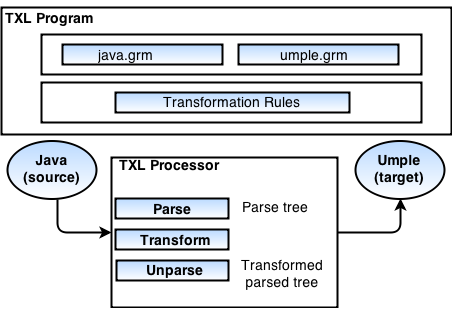
\includegraphics[width=0.75\textwidth]{Figures/TXLprogram.png} 
\caption{TXL program for transforming Java to Umple}
\label{fig:txl}
\end{figure}

\subsubsection{Design Process of the TXL Program}

The first step in writing a source transformer is writing working grammars for both the target and the source language and then writing a union grammar that accepts constructs for both languages. A grammar for Java 1.5 is available from the TXL website \cite{txlresources}. We wrote the grammar for Umple in EBNF format required by the transformation engine. We then built the TXL rules and functions grouped in modules. Each module targets conversion of one specific language construct of Java to the equivalent in Umple and is stored in a separate file. The overall structure of the transformer is shown in Figure \ref{fig:txlStructure}. It contains the modules for the different language constructs and the main program that starts the program. Below, we briefly describe the different modules:

\begin{figure}[h]
\centering
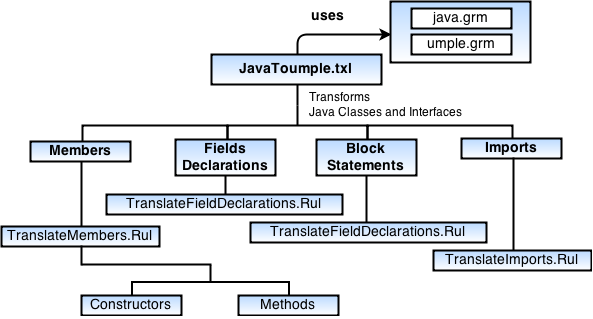
\includegraphics[width=0.98\textwidth]{Figures/TXL_STRUCTURE.png} 
\caption{Structure of the JavaToUmple program}
\label{fig:txlStructure}
\end{figure}

\begin{itemize}
\item JavaToUmple.txl: This is the main program. It is used by TXL to match an input Java program against the Java Grammar and to call the transformation rules.
\item TranslateMembers.rul: Contains rules and functions to transform nested declarations.
\item TranslateFieldDeclarations.rul: Contains rules and functions to transform field declarations.
\item  TranslateBlockStatements.rul: Contains rules and functions for matching bodies of code belonging to constructors and methods.
\item TranslateImports.rul: Contains rules for matching Java imports.
\item TranslateConstructors.rul: transforms the Java constructors.
\item TranslateMethods.rul: transforms Java Methods.
\end{itemize}

The original Java source code remains untouched after applying the transformation. A set of one or more Umple files are produced as a result of the transformation. The \textbf{JavaToUmple} program can be invoked using the command:

\vspace{\baselineskip}
\begin{lstlisting}[style=umplePlain]
< txl –-o outputFileName.ump inputFileName.Java JavaToUmple.txl >
\end{lstlisting}

In the following sub-section we provide some transformation examples. We first show the Java and Umple grammar for the single constructs we transform as well as the TXL transformations rules that guide the transformation.

\subsubsection{Transformation 1: Transforming the Class Header} 

In order to transform a Java class into an Umple class, we need to first transform the class header. The code excerpt in Listing \ref{lst:bnftxl} below shows the EBNF grammar for class definitions in both Java and Umple languages. An example of class definitions is also provided in Listing \ref{lst:sampletxl}.

\begin{lstlisting}[style=umplePlain, caption="Class definition grammar in BNF form", label=lst:bnftxl]
JavaClassDeclaration: 
   ClassModifiers? class Identifier Super? Interfaces? ClassBody


UmpleClassDeclaration: 
   class Identifier ClassBody  ClassBody: '{' ClassContents '}'

\end{lstlisting}

\begin{lstlisting}[style=umplePlain, caption=Class definitions in Java and Umple, label=lst:sampletxl]
// In Java:
public class A extends X implements Z {
    //…some content
}
// In Umple:
class A 
{	
 //.. some content
}
\end{lstlisting}

The mapping rule called `\textit{changeClassHeader}' in file \textit{TranslateMembers.Rul} that transforms class headers of a Java class is presented below in Listing \ref{lst:classHeader}. In order to transform the class header from Java to Umple, we need to deconstruct the class header  (Line 4)  of a Java class and take only what is required in an Umple header, the identifier of the class. The modifiers of the class are discarded and the extends and implements clauses are ignored at this moment, they are analyzed and transformed in subsequent steps of the program transformation. 

\begin{lstlisting}[style=umplePlain, caption=TXL mapping rule for transforming the class headers, label=lst:classHeader]
rule  changeClassHeader 	
   replace $[class_header] 		
    	ClassHead[class_header] 		
    	deconstruct ClassHead 					
    	modifiers[repeat modifier] 'class Name[class_name] 
        ExtendClause[opt extends_clause] 
        ImplmntClause[opt implements_clause]          
    by 	 'class Name 
end rule

\end{lstlisting}

\subsubsection{Transformation 2: Transforming the Package} 

A \textbf{package} in Java can be defined as a grouping of related classes (and types). In Umple a \textbf{namespace} allows to group Umple classes. Listings \ref{lst:txlpackage} and \ref{lst:txlpackage2} show the EBNF grammar of package definition in both languages and an example. 

\noindent\begin{minipage}{.45\textwidth}
\begin{lstlisting}[style=umplePlain,caption=Java package,label=lst:txlpackage]{Name}
PackageDeclaration:
   package PackageName; 

package aPackageName;
\end{lstlisting}
\end{minipage}\hfill
\begin{minipage}{.45\textwidth}
\begin{lstlisting}[style=umplePlain,caption=Umple namespace,label=lst:txlpackage2]{Name}
PackageDeclaration:
   namespace NamespaceName;
 
namespace aNamespaceName;
\end{lstlisting}
\end{minipage}


The mapping rule called `\textit{changePackageToNamespace}' that transforms package declarations is presented below:

\begin{lstlisting}[style=umplePlain, label=lst:packageDeclRule3, caption=TXL mapping rule for the transformation of the package declaration]
rule changePackageToNamespace 
    replace [opt package_header]      
            'package Name [package_name] '; 
    by       
            'namespace Name '; 
end rule	
\end{lstlisting}

\subsubsection{Transformation 3: Transforming the Imports} 

An import declaration in Java allows a named type or a group of named types to be referred to. The `\textit{Depends}' construct in Umple is similar to this. 

\noindent\begin{minipage}{.45\textwidth}
\begin{lstlisting}[style=umplePlain,caption=Java import]{Name}
ImportDeclaration:
     import  QualifiedName; 


import java.io.StreamReader;
public class A {
 //…
}
\end{lstlisting}
\end{minipage}\hfill
\begin{minipage}{.45\textwidth}
\begin{lstlisting}[style=umplePlain,caption=Umple depend]{Name}
DependDeclaration:
   depend QualifiedName;


class A {
  depend java.io.StreamReader;
}
\end{lstlisting}
\end{minipage}

The mapping rule called `\textit{changeImportToDepend}' in file \textit{TranslateImports.Rul} that transforms import declarations is presented below: 

\begin{lstlisting}[style=umplePlain, label=lst:packageDeclRule, caption=TXL mapping rule for the transformation of the import declaration] 
changeImportToDepend  	
    replace [repeat import_declaration]      
           'import Name [imported_name] '; 
    by 	   'depend Name '; 
end rule
\end{lstlisting}

As seen in the example, the depend declarations appear inside the Umple class, so we need additional rules to remove them from the top of the Java class and place them in the right place prior the generation of the Umple code. The rule below removes all the import declarations. The main program, presented next in Listing \ref{lst:removeImportDecls}, illustrates how the program executes the mapping rules in order to produce the output. Note that in TXL, the input program is not modified since the transformation only occurs on the parse tree of the input program.

\begin{lstlisting}[style=umplePlain, label=lst:removeImportDecls, caption=Helper function used to remove the imports declarations] 
function removeImports  
    replace * [package_declaration]
        PkgHead [opt package_header]   
        ImpDecl [repeat import_declaration]  
        TypeDecl [repeat type_declaration] 
    by   
        PkgHead      TypeDecl
end function
\end{lstlisting}


\subsubsection{Final Transformation: The Main Program}

The main program in Listing \ref{lst:mainProgramtxl} is used to execute the three mapping rules presented in the examples above; it calls one by one the rules and the functions and generates the output. Additionally, the main program links, via inclusion constructs, the grammars from the target and source languages (Lines 1-2). In the \textbf{JavaToUmple} program we use two grammar files to map Java and Umple constructs: \textit{Java.grm} and\textit{ Umple.grm}.

\begin{lstlisting}[style=umplePlain, label=lst:mainProgramtxl, caption=The ATL main program - JavaToUmple.Txl] 
include "java.Grm" 
include "Umple.Grm" 

function main    
    replace [program]
        P [program]     
    by 	P [javaToUmple]
end function 

function javaToUmple   
    replace [program] 
         P [program]     
    by 
        P 
        [changePackageToNamespace] 
        [changeImportToDepend] 
        [removeImports] 
        [changeClassHeader]
end function 
% ****	MAPPING RULES HERE   ****
\end{lstlisting}

The transformation program above uses the two grammar files to map Java and Umple constructs:  java.GRM and Umple.GRM. The program rules have been modularized for a better understanding as has been shown in Figure \ref{fig:txlStructure}.

\subsection{ATL}

ATL (ATL Transformation Language) \cite{atl} is a model transformation language that provides ways to produce a set of target models from a set of source models and allows users to define model-to-model transformations in both declarative and imperative ways.

ATL is a set of Eclipse plug-ins created by the Institut National de Recherche en Informatique et en Automatique (INRIA) as an answer to the Object Management Group's QVT language request for proposals \cite{atl}.  The ATL environment in Eclipse offers an ATL editor with syntax highlighting and code completion capabilities, a debugger and a profiler that aims to ease the development and testing of model transformations.

In this section, we describe how queries, views and transformations are handled in ATL. Additionally, we explore the ATL transformations required to umplify a Java system. Figure \ref{fig:atl} presents the necessary components to implement and ATL transformation between Java and Umple. An ATL program (\textit{JavaToUmple.atl} in the Figure) takes model \textit{Java.xmi} as input and produces model \textit{Umple.xmi} as output. Both models need to be expressed in the OMG XMI standard \cite{xmispec}. The Java model conforms to metamodel \textit{Java.ecore} and the Umple model to metamodel \textit{Umple.ecore}. The ecore \cite{ecore} notation is a simple metamodel specification language. The ATL program \textit{JavaToUmple.atl} is also a model, so it conforms to a metamodel (the ATL metamodel). As we will see in Section \ref{subsubsec:exampleATL}, the program is composed of a header, a set of helper functions and a set of (transformation) rules.

\begin{figure}[h]
\centering
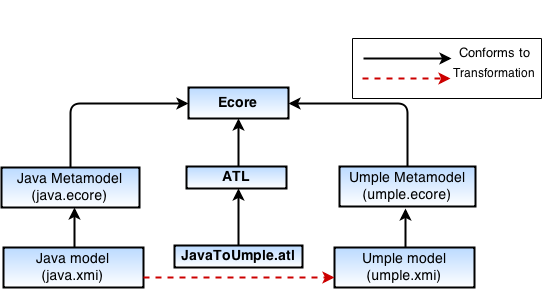
\includegraphics[width=0.75\textwidth]{Figures/ATL_PROGRAM.png} 
\caption{The JavaToUmple ATL program}
\label{fig:atl}
\end{figure}


\subsubsection{The Basics of ATL}

The ATL language is composed of expressions to query model elements (queries), views to handle incremental transformations and transformation rules to direct the transformations of  a set of source models to a set of target models.

\textbf{Queries}

A query in ATL is an expression allowing one to search and return model elements from a model defined in an OMG-compliant format. A query is an OCL expression that can return primitive values, model elements or a combination of these. A query cannot alter the source model. It is possible to navigate across model elements and call query operations on these. For instance, when the following query is executed on a Java model, it first gets the set of all existing JavaElement classes in the model and gets the size of the computed set. The computed integer value is cast into a string before being written into the file `metrics.txt'. 

\vspace{\baselineskip}
\begin{lstlisting}[style=umplePlain]
query JavaElementNb  =
  JavaModel!JavaElement.allInstances()->size().toString()
       .writeTo('metrics.txt')
\end{lstlisting}


\textbf{View}
Views in the ATL world are a special case of transformation. Views offer support for incremental transformations. The user can query a model, perform a transformation on a subset of the source model and save results on a view. Then, she can update the view from its source without executing the whole transformation again. 

\textbf{Transformation Rules}
There are different kinds of rules in ATL based on the way they are called and how they specify the results: matched rules, lazy rules and called rules \cite{stephan2009comparative}.

\begin{itemize}
\item \textbf{Matched Rules}: 	This kind of rule specifies which source element is to be matched, along with the target element that is to be produced.

\item \textbf{Lazy Rules}: This kind of rule is similar to a matched rule, but it is not executed when matched; they rely on being called by other rules.

\item \textbf{Called Rules:}	This kind of rule can have parameters and can be called only from blocks of imperative code. Assignments, `for' and `if' statements are the only three types of (imperative) statements supported in ATL.

\end{itemize}

\subsubsection{ATL Tool Support \textemdash Eclipse M2M}

The ATL project is composed of four parts (or four different plug-ins in Eclipse). The Core, Compiler, Parser and the Virtual Machine (VM) \cite{atl}, which are described below:

\begin{itemize}
\item \textbf{Core} - Contains the classes used to internally represent a model, to allow the creation of models and metamodels, to save and load models and to supply ways to launch the model transformations. 
\item \textbf{Compiler} - Uses the ACG (ATL VM code generator) domain-specific language to compile and generate code. 
\item \textbf{Parser} - Contains all classes to parse an ATL transformation input and to generate an output model compliant with the target metamodel.
\item \textbf{VM} - A byte-code interpreter.
\end{itemize}

\subsubsection{Transformations Examples with ATL}
\label{subsubsec:exampleATL}

In this section we provide some transformation examples in ATL. We present parts of the metamodels, models, mapping rules and the final results (Umple code) of some Java to Umple ATL model transformations.
The JavaModel to UmpleModel examples describe a transformation from a simplified Java Model to an Umple model. 

\paragraph{Metamodels} 

The source metamodel of Java in Figure \ref{fig:javamodelatl} consists principally of \textit{JavaElements} which all have a name. A \textit{JavaClass} has Methods and Fields and belongs to a package. \textit{Methods}, \textit{Fields} and \textit{JavaClasses} are subclasses of the class Modifier and indicate whether they are public, static or final. Java classes and methods declare with the isAbstract attribute whether they are abstract or not. Fields and methods have also a Type. The Java metamodel in Figure 6 has been fully described by the Java Specification \cite{javaSpec} and has been simplified for the purpose of this transformation example.

\begin{figure}[H]
\centering
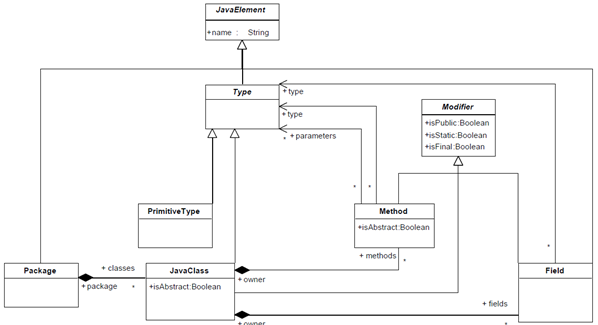
\includegraphics[width=0.99\textwidth]{Figures/javametamodel.png} 
\caption{A simplified version of the Java metamodel}
\label{fig:javamodelatl}
\end{figure}

A simplified version of the Umple metamodel (target metamodel) is presented in Figure \ref{fig:umplemodelatl}. The complete metamodel for Umple can be found at \cite{UmpleMetamodel}. Both metamodels have been defined in the XMI format, as required by the ATL metamodel loader.

\begin{figure}[H]
\centering
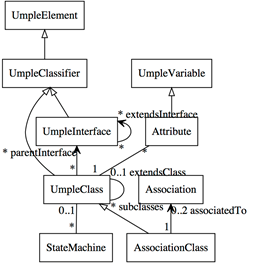
\includegraphics[width=0.55\textwidth]{Figures/umpleMetamodel.png} 
\caption{A simplified version of the Umple metamodel}
\label{fig:umplemodelatl}
\end{figure}

\paragraph{Transformation rules} 

These are the rules to transform a Java Model to an Umple model. The ATL code for the transformation, shown in Listing \ref{lst:atlrules}, consists of several functions and rules. Among the functions, we can mention the \textit{getExtendedName} in Lines 4-8 which recursively explores the namespace to concatenate a full path name.

The three rules presented below are part of the set of rules required to transform a Java Model to an Umple model.  The first rule `\textit{P2P}' in Lines 10-14  specifies how to map a Java package to an Umple namespace. The second rule `\textit{C2C}' in Lines 16-23 declares how we can match a Java Class to an Umple Class. The last rule `\textit{F2A}' aims at transforming a Java Field to an Umple Attribute. This rule is a \textit{called rule} as it is just called whenever a Java Field matches an Umple Attribute. Remember that a Java Field can match an Attribute, Association or State Machine in Umple.

The \textit{FieldHelper} (Lines 29-33) used in rule \textit{F2A} is an utility class used to determine certain properties of a Java field that can derive into properties of a Umple attribute. For instance the \textit{FieldHelper.isLazy(aJavaField)} returns \textit{true} if the Java field passed as parameter is not one of the constructor parameters of its parent class. This helper class is also used to compute components of a Java Field not having a one-to-one match to an Umple class. The (static) method \textit{FieldHelper.getValue(aJavaField)} extracts the value of a field (if any). 

\begin{lstlisting}[style=atl, label=lst:atlrules, caption=ATL transformation rules]
module JavaToUmple;
create OUT: Umple from IN: Java;

helper context Java!Namespace def: getExtendedName() : String = 
	if self.namespace.oclIsUndefined() then '' 	
	else if self.namespace.oclIsKindOf(UML!JavaModel) then 	'' 
	else self.namespace.getExtendedName() + '.'
endif endif + self.name;

rule P2P { 
	from j :Java!Package (e.oclIsTypeOf(Java!Package)) 	
	to out : Umple!Namespace ( 		
			  name <- j.getExtendedName())
}

rule C2C { 	
	from j : Java!JavaClass 	
	to out : Umple!UmpleClass ( 	
			name <- j.name, 	
			isAbstract <- j.isAbstract,      
			// .. parts ignored		
	)
}

rule F2A { 	
	from j : Java!Field to out : Umple!UmpleAttribute ( 		
	name <- j.name,
	value <-  FieldHelper.getValue(j) 	
	isConstant <- FieldHelper.isContant(j), 		
	isImmutable <- FieldHelper.isImmutable(j), 		
	isLazy <- FieldHelper.isLazy(j),
	)
}

\end{lstlisting}

\section{Discussion}

In the previous sections, we demonstrated grammar-based (TXL) and metamodel-based (ATL) transformations for the purpose of umplifying a software system. We showed how to represent the input and output language definitions in both ATL and TXL and how to describe the transformations using rule sets. In this section, we evaluate both transformation approaches to determine whether or not they meet the necessary requirements for implementing the umplification approach. 

Based on the (not-exhaustive) list of requirements presented at the beginning of this chapter in section \ref{sec:ch5Goals}, we now contrast both approaches. The comparison is presented in Table \ref{table:comparisonATLTXL}. The outcomes of our evaluation can have a positive or a negative effect denoted by symbols `+' and `-' respectively. More symbols indicate higher importance  (i.e.  `+++' = high importance, `++' = moderate importance, and `+' = low importance). We will next discuss our rationale for assigning the various levels.

\begin{table}[h]
\centering
\caption{Comparison of ATL and TXL technologies}
\label{table:comparisonATLTXL}
\begin{tabular}{l|p{2cm}|p{2cm}}
\toprule
\rowcolor[HTML]{BBDAFF}
\textbf{Evaluation Criteria} & \textbf{ATL}  & \textbf{TXL}   \\ \midrule
\textbf{Support for various input languages} & - &  -  \\ \hline
\textbf{Incrementality} & - &  -  \\ \hline
\textbf{Rule execution control} & + &   + \\ \hline
\textbf{Command-line support} & - & +++	    \\ \hline
\textbf{Usability of Language} & ++  & +   \\ \hline
\textbf{Rule organization} & +++ &  +++  \\ \hline
\textbf{Output Export} & - &  +++  \\ \hline
\textbf{Maintainability} & + &  ++  \\ \hline
\textbf{Extensibility} & - &  -  \\ 
\bottomrule
\end{tabular}
\end{table}

\paragraph*{Support for various input languages}

In TXL, some of the transformation rules can be reused if our intention is to support a new input source language.  As we described before, to define a model transformation from a new  input language to Umple, we need to:

\begin{enumerate}
\item Construct the working grammar for the input language only since the existing grammar for Umple can be reused. 
\item A union grammar has to be written to combine the source and target grammars. For instance, to combine a grammar rule defining a namespace in PHP and the one defining an Umple namespace, we employ a define statement as follows:

\begin{lstlisting}[style=umplePlain] 
define namespace
 [PHP_namespace] | [Umple_namespace]
end namespace
\end{lstlisting}
The rule above simply means that instances of either PHP namespaces or Umple namespaces can appear during the transformation process. 
\item Build the mapping rules. We require to write all the rules to express the relationship between one pattern in the source  and its transform in the target language. Some logic from the rules aiming at transform other languages could be reused, but in general they have to be completely rewritten. 
\end{enumerate}

In ATL, to support a new input language, we need to:
\begin{enumerate}
\item Create a metamodel definition for the new language to be supported.
\item Create the mapping rules. Some of the logic used in helper functions and rules can be reused but as in the case of TXL, the rules must be written from scratch.
\end{enumerate}

TXL offers a (public) collection of grammars including those for PHP, Java and C++ \cite{txlresources}, therefore reducing the time taken to develop the transformations. 

\paragraph*{Incrementality} 

As discussed in Chapter 3, incrementality means that we possess the ability to perform the transformation in multiple small steps that produce  results quickly. The execution of ATL transformations has always followed a two-step algorithm: 1) matching all rules, 2) applying all matched rules. This algorithm does not support incremental execution. For instance, if a source model is updated, the whole transformation must be executed again to get the updated target model. The only way to implement incrementality in ATL is to regroup the rules belonging to a particular umplification level as lazy rules and then call them from a normal rule. In Listing \ref{lst:lazyRules}, two lazy rules responsible for performing a part of the transformation are called from the rule `transformLevel1'.

\begin{lstlisting}[style=umplePlain, label=lst:lazyRules, caption=Calling lazy rules] 
lazy rule transformAPart {...}
lazy rule transformAnotherPart {...}

rule transformLevel1 {
  from ...
  to umpleClass : umpleMetamodel!UmpleClass { partTransformed <- transformAPart(),
                                              otherPartTransformed <- transformAnotherPart() }
}
\end{lstlisting}

Incrementality in TXL can be achieved  by regrouping the rules belonging to a refactoring level in functions. For instance, `function transform LevelX' regroups all rules that need to be matched (applied) in order to transform the input source at a particular level of refactoring. 

\paragraph*{Rule execution control} 

The order of execution of the transformation rules cannot be explicitly controlled in ATL or TXL. Ordering can be partially controlled as explained above by grouping the rules.

\paragraph*{Command-line support} 

Creating and debugging ATL transformations must be done within the Eclipse IDE. Mapping rules cannot be added on the fly and any rule change requires compiling the entire system. Packaging the transformation files (into a jar) is possible if all Eclipse project dependencies are also packaged. The ATL project offers an Ant task that can be used to chain transformations or to integrate ATL into an existing suite of tools. The major issue when creating a self-contained (and standalone) JAR that can be used in mobile, web applications is that the ATL compiler requires more than 30 dependencies (jars), or bundles as they are called in the Eclipse world. The required bundles are:

\begin{itemize}
\item org.eclipse.ui,
\item org.eclipse.core.runtime;bundle-version="3.4.0",
\item org.eclipse.core.resources;bundle-version="3.4.2",
\item org.eclipse.m2m.*;bundle-version="3.2.1";visibility:=reexport,
\item And other 22 org.eclipse.m2m.* bundles.
\end{itemize}

In addition, the `org.eclipse.core.runtime' requires another 12 dependencies. 

On the other hand, TXL can easily be run on the command-line. 

\paragraph*{Usability of the language} 

In TXL, the language used to define grammars can be easily understood if one has prior knowledge of the BNF notation. In our own experience, the challenge concerns the creation of the rules. The language used to define the patterns and replacements is very rich but also very complex. This is an issue since we continuously need to refine and add more rules. Even with the Java-based Graphical User Interface tool that has been recently developed to help debugging TXL programs, the task is (arguably) complex. 

On the other hand, the ATL language proposes a mix of Java and OCL-like syntax that can be in our opinion easier to understand, even for end-users. 

\paragraph*{Rule organization}

In both TXL and ATL, rules can be properly organized in modules. This improves readability and maintainability.
Similarly, both approaches allow us to separate concerns in a convenient way; grammars and rules can be independently defined, for example.

\paragraph*{Output export} 

%TLFINAL changed ATL to txl in second sentence below
The TXL compiler can generate any type of text file. For instance, a TXL program can generate Umple files (files with extension .ump).

ATL generates only XMI-based models as shown in Listing \ref{lst:atlOutput}. The generated model needs then to be transformed into an Umple model. Listing \ref{lst:atlOutput} shows a generated model containing a class named `Facility' with three attributes (definition omitted).

\begin{lstlisting}[style=umplePlain, label=lst:atlOutput, caption=Model generated by ATL] 
<?xml version="1.0" encoding="UTF-8"?>
<uml:Model xmi:version="2.1" xmlns:xmi="http://schema.omg.org/spec/XMI/2.1" xmlns:ecore="http://www.eclipse.org/emf/2002/Ecore" xmlns:uml="http://www.eclipse.org/uml2/2.1.0/UML" xmi:id="_model" name="model">

  <packagedElement xmi:type="uml:Class" xmi:id="_Facility" name="Facility">
    <ownedAttribute xmi:id="_Facility-id" name="id" visibility="private">
      <type xmi:type="uml:PrimitiveType" href="pathmap://UML_LIBRARIES/UMLPrimitiveTypes.library.uml#Integer"/>
      <upperValue xmi:type="uml:LiteralUnlimitedNatural" xmi:id="_Facility-id-_upperValue" value="1"/>
      <lowerValue xmi:type="uml:LiteralUnlimitedNatural" xmi:id="_Facility-id-_lowerValue" value="1"/>
    </ownedAttribute>
    ....
 </uml:Model>     
\end{lstlisting}

Another issue with ATL is that it requires an input model in  XMI format. To perform a Java-to-Umple transformation in ATL requires transforming the Java source code into XMI, and afterwards transforming the resulting model from XMI into Umple code. Java and C++ to XMI representations can be performed with external tools such as javaML and srcML respectively, but the fact of adding intermediate transformations can considerably affect the overall performance of the transformation tool. Finally, the generated model needs to be transformed using XSLT or similar approaches to an Umple model.

So although ATL and TXL are suitable for certain kind of transformation tasks, as discussed above,  certain concerns cannot be handled naturally when implementing the umplification approach. In fact, the major concerns for any reverse engineering tool used to implement the umplification approach are indeed the extensibility and reusability of the implementation.

To overcome the various issues discussed above, we decided not to use ATL or TXL, and instead use a family of technologies based on `xDT'  (where `x' can be J, P, C, standing respectively for Java, PHP and C/C++), and Drools \cite{Drools_Book}. Each member of the family is intended to deal with a particular kind of transformation task. 

The family of technologies proposed in the following section will improve the following aspects, as compared with what we were able to accomplish with ATL and TXL:

\begin{itemize}
\item Parsing: we employ existing technologies to parse object-oriented source code. These technologies have been proven to work in different contexts and be very reliable. Java, C++ and PHP source code can be parsed with no effort.

\item Visitors: visitors have been developed to traverse the different Abstract Syntax Trees (ASTs) produced by the parsers. This is a required feature to fulfill the requirement for incrementality.

\item Matching: we employ a rule-based engine (Drools) that performs the tasks related to the execution of the rules.

\item Rule definition: the rules are defined using a Java-like language in an editor with syntax-highlighting and code completion capabilities. Visualization and debugging is performed withing the Eclipse IDE. 

\item Exporting capabilities: a custom generator has been developed to output Umple code from an Umple model. Code produced is validated.

\item Command-line capabilities: a self-contained JAR is produced as part of our automated building process. This executable jar is used in an web application currently being developed and for testing purposes.

\item Rule execution: and agenda (a RETE algorithm feature) has been employed to schedule the execution of rules in a deterministic order. 
\end{itemize}


\section{The Umplificator}
\label{chap:tool}
In this section, we provide a detailed description of the tool we have developed to support umplification; as well as discuss some of its technical details.

Our tool, called Umplificator, takes as input  a set of files containing classes written in base language code (Java, C++ etc.), Umple files, source code directories or software projects (source code containers as represented in many popular IDEs such as Eclipse). The output is an Umple textual model containing base language code with modeling abstractions.

At its core, the Umplificator is a language interpreter and static analyzer that parses base language and Umple code/models, populates a concrete syntax graph of the code/model in memory (\textit{JavaModel}, \textit{CPPModel}), performs model transformation on the base language representation in memory and then outputs Umple textual models.

The Umplificator relies on initial parsing by tools such as the Java Development Tool (JDT) for Java, CDT for C++, and PDT for PHP. These extract the input model from base language code. The use of JDT and its siblings reduces the need to write an intermediate parser for the base language.

The base language model is then transformed in a series of steps into an Umple model. To do this, the Umplificator uses a predefined set of refactoring rules written in the Drools rule language \cite{Drools_Book}. Drools is a rule management system with forward- and backward-chaining rules engine. 

The Umplificator includes other subsidiary and internal tools such as:
\begin{itemize}
\item Language validators:  A set of base language validators allowing validation of the base language code that is generated after compilation of the recovered Umple models.
\item Umplificator statistics: A metrics-gathering tool to analyze certain aspects of a software system such as the number of classes and interfaces, the  number of variables present in the code, the cyclomatic complexity, the number of lines of code \cite{MetricsBuse}.  
\item Umplificator Workflow:  A tool that guides the umplification process within Eclipse.
\end{itemize}

The development of the Umplificator follows a test-driven approach to provide confidence that future enhancements will not regress previously functioning and tested aspect of the system. Test-driven testing for the Umplificator is discussed in section \ref{sec:testingUmplificator}. 

\subsection{Architecture}
\label{sec:architecture}

The Umplificator has a layered and pipelined software architecture. The pipelines (components) in this architectural style are arranged so that the output of each element is the input of the next.  Figure \ref{fig:architecture} presents the architecture which is comprised  of four components. The parser, model extractor, transformer and generator components are explained in the following sub-sections.

\begin{figure}[!t]
\centering
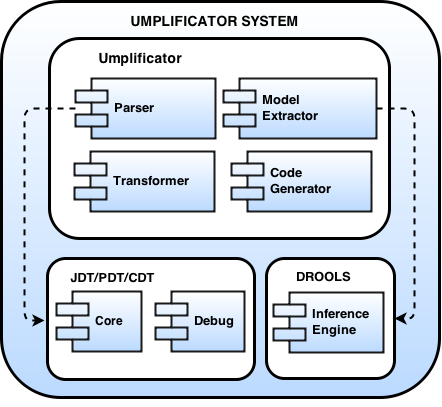
\includegraphics[width=0.75\textwidth]{Figures/UmplificatorComponents.png} 
\caption{The Umplificator components}
\label{fig:architecture}
\end{figure}

The process of umplifying an object-oriented software system in this architecture is described below an illustrated in Figure \ref{fig:process_flow}.

\begin{enumerate}
\item  The input is a set of source code files in the base language and/or Umple.

\item (Parser) The source code is parsed. 

%TLFINAL changed following line
\item (Model Transformer) The source code is transformed into a model of the base language and Umple constructs.

\item (Transformer) The model previously obtained is entered into the next stage of the pipeline. The input model is transformed a model with additional Umple features using pre-defined mapping rules. 

\item The target Umple model, is then validated. 

\item (Generator) Finally, Umple code (.ump files) are generated from the Umple model.
\end{enumerate}

\begin{figure}[!t]
\centering
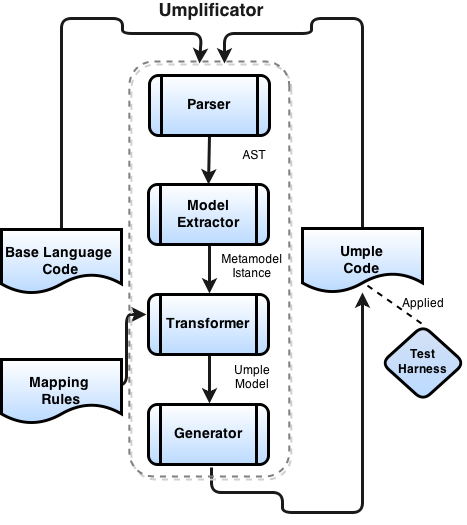
\includegraphics[width=0.75\textwidth]{Figures/Umplificator_ProcessFlow.png} 
\caption{The umplification process flow}
\label{fig:process_flow}
\end{figure}

The Umplificator employs the libraries and technologies summarized in Table \ref{table:technologies} to implement its reverse engineering capabilities. The dependencies between the external and internal components of the Umplificator is shown in Figure \ref{fig:architecture}, where our \textit{Parser} and \textit{ModelExtractor} components uses the JDT/CDT/PDT projects and the \textit{Transformer} the Drools Rule Engine. 

The table also shows which of the components is using the technology. Note that if the technology is used in more than one component, we mark it as `General'.

\begin{table}[h]
\caption{Third party technologies employed in the Umplificator tool}
\label{table:technologies}
\begin{tabular}{l|l|p{6cm}}
\toprule
\rowcolor[HTML]{BBDAFF}
\textbf{Technology} & \textbf{Targeted component(s)}  & \textbf{Description}  \\ \midrule
JDT/CDT/PDT  & Parser and Model Extractor & APIs for parsing object-oriented source code.\\ \hline 
Drools Rule Engine & Transformer  & A Rule Engine for creating and managing the mapping rules used in the Umplificator.	 \\ \hline	
JOpt Simple & General  & Library for parsing command line options \\ \hline	
Log4j & General & A logging library used to collect (reverse-engineering) process data.	\\ \hline	
Perf4j & General & Set of utilities for calculating and displaying performance statistics in the Umplificator code. \\ \bottomrule
\end{tabular}
\end{table}

The different components of the Umplificator as well as the third-party technologies employed are discussed next. 

\subsection{Parser and Model Extractor}

The parser component receives a set of source code files in the base language and/or Umple and creates an abstract syntax tree (AST) as representation of the code. Umple code is allowed as input to allow repeated application to refine the model. To implement its parsing and base language model extraction capabilities, the Umplificator uses various Eclipse Projects, as summarized in the following table. These projects provide APIs to access and manipulate object-oriented source code.
They also provide access to the  source code via two different means: a base language model within the Eclipse Workspace and an Abstract Syntax Tree (AST) for a standalone usage (outside the Eclipse IDE). Table \ref{table:xdtProjects} summarizes the Eclipse projects used in the Umplificator for parsing purposes. We then provide some details about the capabilities and usage of each project. 

\begin{table}[ht]
\caption{Eclipse projects used in the Umplificator}
\label{table:xdtProjects}
\begin{tabular}{l|p{4cm}p{5cm}}
\toprule
\rowcolor[HTML]{BBDAFF}
\textbf{Project} & \textbf{Targeted programming language}  & \textbf{Components used (plug--ins)}  \\ \hline
	Java Development Tooling & Java   & org.eclipse.jdt.core , org.eclipse.jdt.core.dom  \\ \hline
	C++ Development Tooling  & C++   & org.eclipse.cdt.core \\ \hline
	PHP Development Tools	 & PHP   & org.eclipse.pdt.core \\ \hline
\end{tabular}
\end{table}

Eclipse is not simply a programming language IDE. In fact,  Eclipse is an extensible platform for building IDEs. Eclipse functionality is wrapped into pluggable components called \textit{plug-ins}. These plug-ins allow developers to extend the basic functionality offered by Eclipse. The projects mentioned in the above table, are plug-ins that can be used in other projects inside Eclipse or as a standalone component, as in our case.

Architecturally, the JDT/CDT/PDT projects are divided into two domains: the model (core) and the user interface. The model is a representation of the Base language elements; the user interface is a set of views, actions, perspectives and menus that work together. The user interface domain can be extended but only works inside Eclipse (not intended for standalone usage).  The Umplificator uses the model component of these projects to \textit{parse} and \textit{extract} a base language model from source code. 

\paragraph*{Java Development Tooling (JDT)}

 Eclipse Java Development Tooling (JDT) \cite{jdtProject} offers a comprehensive Java development environment. JDT also provides APIs for analyzing Java source code. It provides several levels of source code analysis that can be reused. The level of source code analysis used in the Umplificator is the Abstract Syntax Tree (AST) framework. We use the AST to analyze the Java source code as a tree of nodes, where each node represents a part of the source code (for instance a variable declaration, a method body, a contructor and so on). The AST framework defines over 60 \textit{ASTNode} \cite{astnodeapi} subclasses representing the different elements of the Java language. 
 
% I dpn't get 'over ASTNODE' above
% MG. Over 60 subclasses...
  
The AST framework includes also interfaces that help retrieve specific source information beyond what is indicated by the ASTNode source pointers. To traverse the nodes returned by the parser (ASTParser) and collect the desired information about the source code, we employ multiple visitor classes that follows the Visitor software design pattern \cite{gamma1994design}. 
The visitor pattern is a standard way to decouple the data from the operations that process the data.
For each different AST node type T, two methods are offered:

\begin{itemize}

\item  \textit{public boolean visit(T node)} -- Visits the given node to perform some arbitrary operation. If true is returned, the given node's child nodes will be visited next;
\item  \textit{public void endVisit(T node)} --  This method is called after all of the given node's children have been visited (or immediately, if visit returned false). The default implementation provided by this class does nothing;
\end{itemize}

Generally, the AST visitor can be used to \textbf{transform} AST nodes or to \textbf{derive} information. A derivation collects information and stores result along the way. For instance, if our intention is just to collect the import declarations of a Java class, we could write a visitor as in Listing \ref{lst:importvisitor}. In the method visit(...) we return false to stop the visitor from visiting child nodes of the import declaration. The variable \textit{importDeclarations} is an array containing the (visited) import declarations. 

\begin{lstlisting}[style=java, caption=A visitor for import declarations in Java source code, label=lst:importvisitor]

public class SimpleVisitor extends ASTVisitor{

	private List<ImportDeclaration> importDeclarations;

	public boolean visit(ImportDeclaration node) {
	    importDeclarations.add(node);
	    return false;
	}
}
\end{lstlisting}

As an example, consider the code of class `\textit{Test}' in Listing \ref{lst:astjava}. Once the code is parsed, we used a visitor to collect the desired information. Table \ref{table:astanalysis} presents the resulting AST node types, the corresponding source fragment and the visitor employed to collect the information. This table recapitulates the entire process of parsing and extracting the model for our sample code. 


\begin{lstlisting}[style=java, caption=Test.java, label=lst:astjava]
package umplificatorTest;

import java.util.Date;

public class Test {
	public int number;
	
	public int  getNumber() {
		return number;
	}
}
\end{lstlisting}

\newcommand*{\MyIndent}{\hspace*{0.4cm}}%
\begin{table}[h]
\caption{Sample uses of an AST for code analysis}
\label{table:astanalysis}
\begin{tabular}{l|p{4cm}p{4cm}}
\toprule
\rowcolor[HTML]{BBDAFF}
\textbf{ASTNode Type} & \textbf{Source Fragment}  & \textbf{Visitor Code}  \\ \midrule	
\textbf{CompilationUnit} &  Entire source code & visit(CompilationUnit cu) \\ \hline
\MyIndent \textbf{PackageDeclaration}& ``package umplificatorTest" & visit(PackageDeclaration pd) \\ \hline
\MyIndent \textbf{ImportDeclaration} & ``import java.util.Date" & visit(PackageDeclaration pd) \\ \hline
\MyIndent \textbf{TypeDeclaration} &  ``public class Test" & visit(TypeDeclaration td) \\ \hline
\MyIndent \MyIndent \textbf{FieldDeclaration} &  ``public String name" & visit(FieldDeclaration fd) \\ 
\MyIndent \MyIndent \MyIndent PrimitiveType(``int") &   &  td.getType() \\ 
\MyIndent \MyIndent \MyIndent SimpleName(``number") &   &  td.getSimpleName() \\ \hline
\MyIndent \MyIndent \textbf{MethodDeclaration} &  ``public int getNumber()" & visit(MethodDeclaration md) \\ 
\MyIndent \MyIndent \MyIndent PrimitiveType(``int") &   &  td.getReturnType() \\ 
\MyIndent \MyIndent \MyIndent SimpleName(``getNumber") &   &  td.getName() \\ \hline
\MyIndent \MyIndent \MyIndent \MyIndent \textbf{Block} & ``{..}"& bl=  md.getBody() \\ 
\MyIndent \MyIndent \MyIndent  \MyIndent \MyIndent \textbf{ReturnStatement} &  ``return number;" & stmt = b1.getStatements(0); \\ \bottomrule
\end{tabular}
\end{table}

Note that the AST node type CompilationUnit is the type root of an AST (first row of above table) and the object returned by the ASTParser after completion of the parsing a Java file. The source range for the CompilationUnit type node is the entire source file, including leading and trailing whitespace and comments. In Java 1.4 to 1.7, a CompilationUnit is composed of 
a \textit{PackageDeclaration}, \textit{ImportDeclaration}, and one or more of these types:  \textit{TypeDeclaration}, \textit{EnumDeclaration}, \textit{AnnotationTypeDeclaration}. 
%FINAL CHANGE START
Code comments, which are important from an understanding viewpoint, are preserved in the AST, parsed and transformed into Umple comments. \textit{Comment}, is the abstract base class for all AST nodes that represent comments. There are exactly three kinds of comments: line comments (\textit{LineComment}), block comments (\textit{BlockComment}), and doc comments (\textit{Javadoc}).
%FINAL CHANGE END
%TLFINAL added space below

The code on the right of Table \ref{table:astanalysis} shows several examples of what can be done inside a visitor method:

% change the phrasing below to avoid the second person 'you'. i.e. get rid of 'Do you 
% MG FIXED
\begin{itemize}
\item Extracting the name of the package: Code a \textit{visit(PackageDeclaration)} and get its name as an instance of \textit{SimpleName} (e.g. package test)  or \textit{QualifiedName} (e.g. package cruise.compiler.*).
\item Getting the list of types referenced in a compilation unit? Code a \textit{visit(TypeDeclaration)} and get theirs names as instances of \textit{Simple} or \textit{QualifiedName}.
\item Finding all literal integers referenced only within methods and not fields? Code a `sub' \textit{visit(IntegerLiteral)} inside the visit method for \textit{MethodDeclaration}.
\end{itemize}

\paragraph*{C/C++ Development Tooling (CDT)}

In the same manner as the JDT technology and using the same concepts for parsing an model extraction, the CDT provides powerful features to analyze code in C and C++. CDT contains two parsers, for C and C++, that generate an AST representation from source code. The CDT project, as we have explained for JDT, is a set of plug-ins that adds full support for parsing, analyzing and developing C/C++ applications. The Umplificator uses the core component of CDT to implement its reverse engineering capabilities (org.eclipse.cdt.core). The following are some of the CDT core features that are used in the Umplificator:

\begin{itemize}
\item \textbf{Preprocessor}: Converts source code text into a token stream and evaluates inclusion directives and macros. The preprocessor phase runs before the parser. 
\item \textbf{Parser}: Converts the token stream into an AST
\item \textbf{AST}: Used to traverse and collect information about the source code (CPPModel). A visitor API is also provided. 
\item \textbf{AST Rewrite API}: Used to implement refactoring (method refactoring mostly).
\end{itemize}

The CDT supports the different C++ language constructs such as multiple inheritance, templates, header files, etc.
The AST represents the structure of source code, as it was the case for JDT.  One of the main differences between CDT and JDT is that the root object returned by the ASTParser is the `\textit{TranslationUnit}' and not a `\textit{CompilationUnit}'. 
A TranslationUnit (CDT) is assembled from multiple source files, a CompilationUnit (JDT) represents a unique Java file.
For instance, the very simple program in Listing \ref{lst:cdtsimple} printing a string in the console, when compiled produces more than 1000 lines due to inclusion of header file `stdio.h' (\textless gcc -E test.c | wc -l \textgreater returns 1052).

\begin{lstlisting}[style=java, caption=Simple example in C++ - test.c , label=lst:cdtsimple]
#include <stdio.h>
int main() {
	printf("Hello World\n");
}
\end{lstlisting}

Comments are preserved in the AST and can be accessed as comment nodes.

\paragraph*{PHP Development Tooling (PDT)}

The PHP Development Tools (PDT) is a toolset intended to encompass all tools necessary to develop PHP based software. 
It provides the primary modules: the core, the debug and the user interface. The \textit{core} component is, as in the previous cases, used in the Umplificator to parser and analyze PHP source code.
We will not provide further detail on the PDT, since it follows the same architecture and model extraction concepts that we have already covered in the discussion of JDT and CDT Eclipse technologies.

To recapitulate this sub-section, the \textit{parser} component of the Umplificator, leveraging various parsing technologies, parses source code, creates a AST representation of the code that is traversed by the \textit{model extractor} to finally obtain a base language model. The base language model is then traversed using a series of visitors. The input/output relationship of the parser and model extractor components is illustrated in Figure \ref{fig:parserINOut}. 

\begin{figure}[h]
\centering
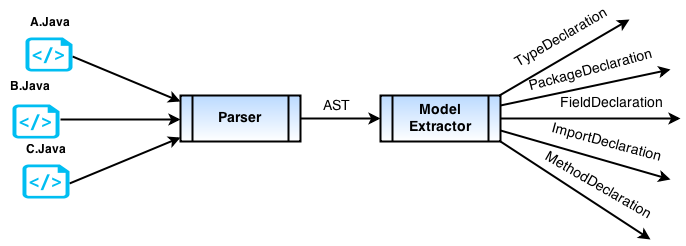
\includegraphics[width=0.98\textwidth]{Figures/parserINOut.png}
\caption{The Parser and Model extractor components}
\label{fig:parserINOut}
\end{figure}

\subsection{Transformer}

The core of the tool suite is the Transformer. The Transformer receives a base language model (e.g. JavaModel, CPPModel or PHPModel) from the extractor and an empty Umple model which is then populated. In fact, the base language model is decomposed into a series of objects representing each particular piece of the source code (a package, an import, a field and so on). Furthermore, the base-language model is transformed using a predefined set of mapping rules. If the input model is Umple code, the transformer produces an Umple model with additional modeling constructs (abstractions). The input/output relationship for the Transformer component is illustrated in Figure 
\ref{fig:transformerInOut}.

\begin{figure}[h]
\centering
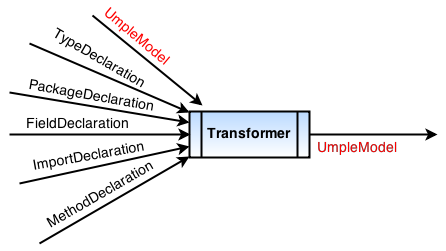
\includegraphics[width=0.70\textwidth]{Figures/transformerINOut.png}
\caption{The Transformer component inputs and outputs}
\label{fig:transformerInOut}
\end{figure}

As we have seen in Table \ref{table:technologies}, the Transformer component leverages Drools technologies to implement its rule engine.

\subsubsection{Drools Rule Engine}

The rule engine interprets and executes the mapping rules on the source model and target model to produce the umplified version of the target model.
The Drools engine used by the Umplificator is composed of an inference engine that is able to scale to a large number of rules and facts.  The inference component matches facts and data (base language models) against rules to infer conclusions, which result in actions (model transformations). A rule is a two-part structure (Left-hand-side part and Right-hand-side part) using first order logic for reasoning over knowledge representation.

At a high-level structural view, the Rule Engine consists of a: an \textit{Inference Engine}, an \textit{Agenda}, a \textit{Pattern Matcher}, a \textit{Production Memory} and \textit{Working Memory}. 
The rules are stored in the \textit{Production Memory} and the facts that the Inference Engine matches against are kept in the \textit{Working Memory}.
Facts are the data on which the rules act (model elements in our case).
Pattern matching is performed to match facts against rules and is implemented using the Rete algorithm \cite{reteDROOLS}. Facts are evaluated into the Working Memory where they may be modified or retracted. The \textit{Agenda} manages the execution order of the rules. Figure \ref{fig:RuleEngineArchitecture} shows the difference components of the Rule Engine.

\begin{figure}[h]
\centering
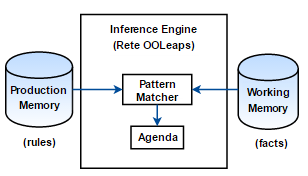
\includegraphics[width=0.75\textwidth]{Figures/RuleEngineArchitecture.png}
\caption{High level view of the Drools rule engine}
\label{fig:RuleEngineArchitecture}
\end{figure}

Traditionally, rule engines have two methods of execution \cite{RulebasedSystems} forward chaining and backward chaining. In forward chaining, the facts are asserted into working memory resulting in one or more rules being concurrently true and scheduled for execution. In backward chaining (goal driven), one starts with a conclusion, which the engine tries to satisfy. Drools is a Hybrid Chaining System because it implements both forward and backward mechanisms. Our Umplificator uses the forward chaining method of operation in which the inference engine starts with facts, propagates through the rules, and produces a conclusion (e.g. a transformation). Figure \ref{fig:backwardForward} contrasts the two modes of execution. In Forward Chaining, the engine discovers what conclusions can be derived from the data and asserts them (iteratively), whereas in Backward chaining the engine starts with the goals and searches how to satisfy them (as in Prolog).


Consider the scenario of a model transformation in Figure \ref{fig:backwardForward}: if the conditions C1,C2 and C3 apply on a base language element, then we can perform the transformation as dictated by D1. 
On the other hand, in backward chaining, we perform the transformation and then attempt to determine if it was correct based on the available information (C1,C2,C3 and input model element).

\begin{figure}[h]
\centering
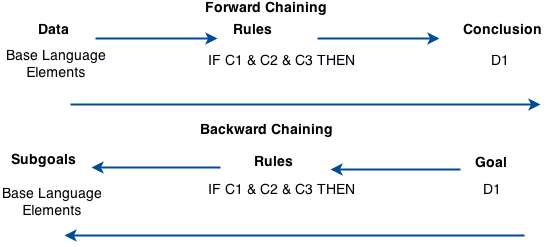
\includegraphics[width=0.80\textwidth]{Figures/ForwardBackwardChaining.png}
\caption{Forward vs backward chaining}
\label{fig:backwardForward}
\end{figure}

\subsubsection{The Rule Language}
The rule engine is initialized with the rules. Drools offers a native rule language, very light in terms of punctuation and supporting Java and domain-specific languages. 

A rule file in Drools (and in our implementation) is a file with a .drl extension that can have the following elements:

\begin{itemize}
\item \textbf{Package}: The package name, if declared, must be the first element in the rule file and represents the namespace, which is kept unique for a given grouping of rules.
\item \textbf{Imports}: These are used to import Java types referenced by the rules.
\item \textbf{Global Variables:} A global variable is a variable visible to all the rules inside a rule file. These are not inserted into the Working Memory and are most commonly used to log information on the execution of rules.
\item \textbf{Functions}: These are used for invoking actions on the consequence (then) part of the rule, especially if that particular action is used over and over again. 
\item \textbf{Queries}: These provide a means to search working memory and store the results under a named value. In the Umplificator, they are used to gather metrics information about the models analyzed. For instance, the query  numberOfPublicMethods(...) returns the number of methods having `public' as modifier. Queries do not have side effects, meaning that their evaluation cannot alter the state of the corresponding executing unit. 
\end{itemize}

The rules, as explained in this section, are instructions indicating how a piece of the Base language model (Java Model, C++ model, etc.) is mapped to a piece of an Umple model. In the Umplificator, the logic used for model transformations resides in the rules. Moreover, by using rules, we have a single point of truth, a centralized repository of knowledge. Rules can be also read and understood easily, so they can also serve as documentation.

Listing \ref{lst:droolsrule} shows the basic form of a rule in Drools language, where LHS is the conditional part of the rule and RHS is a block that allows dialect-specific semantic code to be executed.  Attributes (Line 2) provide a declarative way to influence the behavior of the rule. We present the rule attributes used in our mapping rules in Table \ref{table:ruleattributes}.

% Refer to the listing number since a figure could get in the way
% MG FIXED
\begin{lstlisting}[language={drools},label={lst:droolsrule}, caption=Basic rule in Drools] 
rule "name" 
  attributes 
  when LHS then RHS
end
\end{lstlisting}

\begin{table}[h]
\caption{Rule attributes}
\centering
\label{table:ruleattributes}
\begin{tabular}{l|p{9cm}}
\toprule
\rowcolor[HTML]{BBDAFF}
\textbf{Attribute Name} & \textbf{Description}   \\ \midrule
\textbf{no loop} & Avoids infinite loops. When a rule's consequence modifies a fact it may cause the rule to activate again, causing an infinite loop; its default value is false.\\ \hline
\textbf{lock-on-active} &  Stronger version of no-loop. If a rule declares this attribute, the rule can be activated once.   \\ \hline
\textbf{Salience} & Salience is a form of priority where rules with higher salience values are given higher priority when ordered in the Activation queue; its default value is 0. \\ \hline
\textbf{agenda-group} & Agenda groups allow the user to partition the Agenda providing more execution control. Only rules in the agenda group that have acquired the focus are allowed to fire.     \\ \bottomrule
\end{tabular}
\end{table}

\textbf{Order of execution and grouping}

The rules are grouped in files for each of the cases (levels of refactoring) discussed earlier. In other words, there is a rule file containing rules, functions and queries to transform classes, namespace and imports; another file containing those to transform variables into attributes, another file containing those to transform variables into associations and so on.

To activate the groups on the required order, we used agenda groups. Agenda groups are a way to partition the activation. At any one time, only one group has `focus', meaning that activation for rules in that group will take effect. 
In other words, agenda groups provide a way to create a flow between grouped rules. They work as a stack. When we set the focus to a given agenda group, that group is placed on top of the stack. When the engine tries to fire the next activation and there are no more activations in a given group, that group is removed from the top of the stack and the group below receives focus again.

The Umplificator executes the rules to transform classes first, followed by the rules transforming attributes and finally by the rules transforming associations. 

We use the attribute agenda-group in the rules to specify the order of the activation. For instance, the rule in Listing \ref{lst:agendagroup} is a rule belonging to the group that will be executed first. The rule in Listing \ref{lst:agendagroup2} will be executed after any rule belonging to the first level. 

\begin{lstlisting}[language={drools},label={lst:agendagroup}, caption=A rule belonging to Level 1] 
rule "transform_Namespace_UInterface"
	agenda-group "LEVEL1" 
	when
	// parts omitted
	then
	// parts omitted
end
\end{lstlisting}

\begin{lstlisting}[language={drools},label={lst:agendagroup2}, caption=A rule belonging to Level 2] 
rule "JavaField_CanBeUmpleAttribute"
	agenda-group "LEVEL2" 
	when
	// parts omitted
	then
	// parts omitted
end
\end{lstlisting}

Listing \ref{lst:fireAllRules} shows how the rules are inserted into the Working Memory of the Umplificator rule engine. Level 3 will be put on the bottom of the stack, followed by Level 2 rules, and Level 1 rules which will be on the top of the stack. The \textit{KieSession} object represents the working memory of the Rule Engine.

\begin{lstlisting}[style=java, caption=Firing the rules in the Umplificator, label=lst:fireAllRules]
public KieSession fireAllRules()
{
// Agenda works as a stack
kieSession.getAgenda().getAgendaGroup( "LEVEL3" ).setFocus();
kieSession.getAgenda().getAgendaGroup( "LEVEL2" ).setFocus();
kieSession.getAgenda().getAgendaGroup( "LEVEL1" ).setFocus();
kieSession.fireAllRules();

return kieSession;
}
\end{lstlisting}

More details on the different mapping rules will be presented in Section \ref{sec:automatedUmplification}.

\subsection{Generator}

The Generator component validates the received UmpleModel and generates Umple code from it. That is, it generates an Umple file for each class or interface in the Umple model.

\begin{figure}[h]
\centering
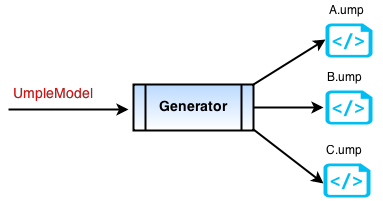
\includegraphics[width=0.55\textwidth]{Figures/generatorINOut.png}
\caption{The Generator component inputs and outputs}
\label{fig:generatorInOut}
\end{figure}

The Generate supports different options when it comes to generation of output files.  One way to do this is to follow the Java convention of having one .ump file per class. Another common approach is to have one or more files for the model code (just the pure UML elements such as classes with their attributes, associations and state machines) and separate files for the methods; we can in fact have some files for Java methods, and other files for PHP or C++ methods. The same model can then be used to develop systems that are deployed in multiple base languages. For instance, for the Java  input class\textit{A.java}, the two following files would be generated:

\begin{enumerate}
\item \textit{A.ump}: containing methods, algorithmic and logic code for class A.
\item \textit{A\_model.ump}: Modeling constructs for class A.
\end{enumerate}

The Generator supports also the creation of directories to preserve the namespace structure. For instance, if the namespace of the Umple file is `cruise.Umple', the Generator will create two directories, `cruise' and `Umple' (inside).

\section{Summary of Umplification Technologies}

In the previous sections, we have presented the current implementation of the umplification approach. The Umplificator employs different technologies to deal with the various tasks of the umplification process. 
The advantages of our mixed approach are enumerated below:

\begin{description}
\item [Separation of concerns] The Rule-Engine allows us to break the coupling between the data and logic. The logic is all laid out in rules. With the use of rules, we solve the issues related to hand-coded `if..then' approaches.

\item [Speed and scalability] The Rete algorithm provides very efficient ways of matching rule patterns to the internal representations of the input source code. In addition, the Rete algorithm has been proven to be highly scalable. This is important to meet the requirements of industrial projects, where large-scale models must be dealt with.

\item [Centralization of knowledge] The different rules form a repository of knowledge that serves as a single point of truth. The rules are readable enough to be used as documentation. 

\item [Multi-level testing] Each component in our implementation can be independently tested. This is further discussed in the next chapter of this thesis. Tests can reveal if the addition of rules (or refinements) have invalidated existing transformations.

\item [Robust parsing] The CDT, JDT and PDT parsers are robust and well-maintained. This is very desired characteristics since languages like Java and C++ are in continuous development. For instance, JDT has been updated to comply with the different Java versions, from 1.4 to 1.8. In addition, the parsers are able to parse specific parts of the code (a method, a constructor, etc). This is a desired feature to comply with the incrementality requirements of the umplification approach. 

\item [Efficiency] The parsing technologies employed are industrial technologies that have been validated with large systems. For instance, Piatov et al. in his study \cite{CDTPARSER}, has concluded that the CDT parser is a robust, efficient and actively maintained parsing technology. 

\item [Agile development] The process of building transformations as it stands in our current implementation is compatible with the practices and principles of agile development which are of growing importance in software engineering \cite{agileDev} and systems engineering.

\item [Extensibility] Rule files (files with extension .drl) can be added on the fly without requiring re-compilation of the entire Umplificator. End-users can then add more rules for their specific needs. 

\item [Reusability] Pattern-matching conditions and actions in (Drools) rules can be reused to accommodate new transformations for different languages. 
\end{description}
%FINAL CHANGE START
Furthermore, the estimated cost of our implementation, calculated using the \textit{COCOMO model} \cite{COCOMO}, with coefficients a=2.4 and b=1.05, is:

\begin{itemize}
\item \textit{Codebase Size}:   114725 LOC
\item \textit{Duration} = 23.27 months
\item \textit{Effort} = 1066.33 person-months
\end{itemize}
%FINAL CHANGE END
%TLFINAL changed slash to hyphen in person-months

\section{Automated Umplification Example}
\label{sec:automatedUmplification}
\subsection{Initial transformation}

As an example of the transformation process using the Umplificator, consider the input Java source code in Listing \ref{lst:exampleTransformer}.
We want to achieve the initial level of refactoring (Level 1).

\begin{lstlisting}[style=java, caption=Input source code, label=lst:exampleTransformer]
package university;

import java.util.Date;

public class Student {
	
    private String name;
    private int studentId;
    
    public Student (int studentId) {
    	this.studentId = studentId;
    }
    public String getName () { return name;}
    
    public void  setName (String aName) { 
    	this.name =  aName;
    }
   
    public int getStudentId () { return studentId;}
    
    public String toString() {
    	return "The student " + name "has id=" + studentId;
    }
}   
\end{lstlisting}

The \textit{Parser} receives the source code above, creates an Abstract Syntax Tree representation of it and transfers it to the Model Extractor. The Model Extractor uses the AST representation to create a Java model which is then traversed and decomposed in pieces by means of a Java class visitor. Table \ref{table:exampleTransformer} presents all the Java Elements collected by the Java visitor.

\begin{table}[h]
\caption{The input Java Model elements}
\label{table:exampleTransformer}
\centering
\begin{tabular}{l|l}
\toprule
\rowcolor[HTML]{BBDAFF}
\textbf{ASTNode Type} & \textbf{Source Fragment}  \\ \hline	
\textbf{PackageDeclaration} & "package university;" \\ \hline
\textbf{ImportDeclaration} & "import java.util.Date;" \\ \hline
\textbf{TypeDeclaration} &  "public class Student"  \\ \hline
\MyIndent \textbf{FieldDeclaration} &  "public String name;"  \\ \hline
\MyIndent \textbf{FieldDeclaration} &   "public int studentId;"  \\ \hline
\MyIndent \textbf{MethodDeclaration} &  "public int getStudentId () {...}"  \\ \hline
\MyIndent \textbf{MethodDeclaration} &  "public String getName () {...}"  \\ \hline
\MyIndent \textbf{MethodDeclaration} &  "public void  setName(...) {}"  \\ \hline
\MyIndent \textbf{MethodDeclaration} &  "public Student(...){}"  \\ \hline
\MyIndent \textbf{MethodDeclaration} &  "public String toString(){...}"  \\ \hline
\end{tabular}
\end{table}

The Transformer receives the Java model elements in Table \ref{table:exampleTransformer}, together with a newly created instance of an UmpleModel and places them into the Working Memory.  At this point of time, the \textit{Production Memory} contains all rules  but the \textit{Agenda} contains only those belonging to this level of refactoring (those with attribute `agenda-group LEVEL1'). 

When the model elements (facts) are inserted into the memory, the pattern matching begins. The rule engine then tries to find objects matching the conditions in the rules. The only rule meeting all the conditions and that can be matched to objects in the Working Memory is the rule named \textit{addClassToUmpleModel}. The rule is presented in Listing \ref{lst:addClassToUmpleModel}.

\begin{lstlisting}[language={drools},label={lst:addClassToUmpleModel}, caption=Rule 'addClassToUmpleModel']
rule "addClassToUmpleModel"
 agenda-group "LEVEL1" 
 when
  typeDeclaration: TypeDeclaration()
  umpleModel: UmpleModel()
 then
  String typeName = getTypeDeclarationName(typeDeclaration);
  UmpleClass umpleClass = new UmpleClass(typeName);
  umpleModel.addUmpleClass(umpleClass);
  insert(umpleClass);
end
\end{lstlisting}

The rule above simply requires the presence in the Working Memory of an instance of TypeDeclaration (Line 4) and an instance of an UmpleModel (Line 5). As the conditions are satisfied, in the RHS of this rule we create a new instance of UmpleClass, setting its name. To extract the name of the instance \textit{TypeDeclaration} we employ a helper function \textit{getTypeDeclarationName(...)}. After the object is created, we insert it into the session with the `\textit{insert(umpleClass)}' method. This process of matching facts with rules (i.e. inference) is illustrated in Figure \ref{fig:ruleModel}.

\begin{figure}[h]
\centering
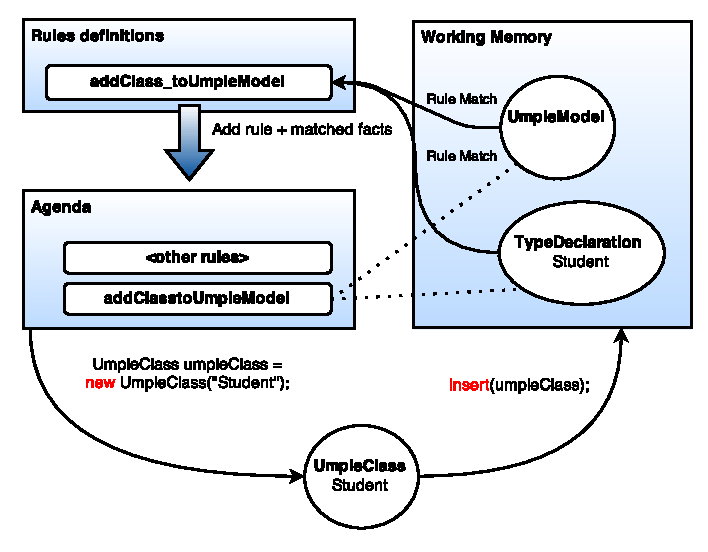
\includegraphics[width=0.98\textwidth]{Figures/ruleModel.pdf}
\caption{Pattern matching and creation of an UmpleClass}
\label{fig:ruleModel}
\end{figure}

After the insertion of the UmpleClass into the working memory, the inserted object can generate more rule matches. The UmpleModel residing in the Working Memory now contains one Umple class. It is automatically updated by the engine.

The rules for the remaining Umple class constructs are then matched. The goal of these rules is to populate the Umple class based on the information obtained from the typeDeclaration. 

The rule named \textit{transformImportDeclaration} (Lines 1-11) in Listing \ref{lst:ruleImport} matches and converts any Import Declaration (Java Language) into an Umple depend construct. The dependency (Line 9) is then added to a matched Umple Class. The Umple Class residing in the Working Memory is then updated at Line 10.

To ensure that the dependency is not added to any \textit{umpleClass} in the Working Memory but only to the one owning it, we assert that the ImportDeclaration's parent class has the same name as our targeted UmpleClass. The helper function, imported in the first line of the above Listing, is a static function that returns the name of the parent class of the ImportDeclaration. In our case, the name of parent Java class is ``Student'' which corresponds to the name of a UmpleClass in memory. The `eval' clause returns true in this particular case.

\begin{lstlisting}[language={drools},label={lst:ruleImport}, caption=Rule transformImportDeclaration]
import function cruise.umplificator.rules
       .TopLevelAnalyzerHelper.getDeclarationContainerName
      
rule "transformImportDeclaration"
 agenda-group "LEVEL1" 
 when
  importDeclaration: ImportDeclaration()
  uClass: UmpleClass()
  eval(uClass.getName()
       .equals(getDeclarationContainerName(importDeclaration)))		
 then
  Depend depend = new Depend(getImportName(importDeclaration));
  uClass.addDepend(depend);
  update(uClass);
 end
\end{lstlisting}

The package declaration is converted then into a namespace with the rule `transformNamespace' in Listing \ref{lst:transformNamespace}. We again ensure that the package declaration corresponds to the targeted UmpleClass. Note that in this rule we do not need to insert the namespace object into memory since we do not expect any rule to match it.

\begin{lstlisting}[language={drools},label={lst:transformNamespace}, caption=Rule transformNamespace]
import function cruise.umplificator.rules
       .TopLevelAnalyzerHelper.getDeclarationContainerName
rule "transform_Namespace"
 agenda-group "LEVEL1" 
 when
  packageDeclaration: PackageDeclaration()
  uClass: UmpleClass()
  eval(uClass.getName()
      .equals(getDeclarationContainerName(packageDeclaration)))	
 then
  uClass.addNamespace(packageDeclaration.getName()
                      .getFullyQualifiedName());
end
\end{lstlisting}

As we have assumed an initial level of refactoring, at the beginning of this example, the Transformer will not attempt to transform any variable into an Umple attribute, or association end. However, in the final output code produced for our UmpleClass we require the remaining untreated code to be simply appended. For instance, the rule `appendFieldDeclaration' in Listing \ref{lst:appendField} extracts information from the field declaration and appends it to the targeted Umple Class. The same behavior is produced from the application of rule `appendMethodDeclaration' in Listing \ref{lst:appendMethod}.

\begin{lstlisting}[language={drools},label={lst:appendField}, caption=Rule appendFieldDeclaration]
import function cruise.umplificator.rules
       .TopLevelAnalyzerHelper.getDeclarationContainerName
       
rule "appendFieldDeclaration"
 agenda-group "LEVEL1" 
 when
  fieldDeclaration: FieldDeclaration()
  uClass: UmpleClass()
  eval(uClass.getName()
       .equals(getDeclarationContainerName(fieldDeclaration)))
  eval(!uClass.getExtraCode().contains(fieldDeclaration.toString()))
 then
  uClass.appendExtraCode(fieldDeclaration.toString());
  update(uClass);
end
\end{lstlisting}

The \textit{eval} clauses in Listing \ref{lst:appendField}, ensure that the string representing the field information has not been appended before and (as before) that the field string is added to the Umple class owning it.

\begin{lstlisting}[language={drools},label={lst:appendMethod}, caption=Rule appendMethodDeclaration]
import function cruise.umplificator.rules
       .TopLevelAnalyzerHelper.getDeclarationContainerName
       
rule "appendMethodDeclaration"
 agenda-group "LEVEL1" 
 when
  method: MethodDeclaration()
  uClass: UmpleClass()
  eval(uClass.getName().equals(getDeclarationContainerName(method)))
  eval(!uClass.getExtraCode().contains(method.toString()))
 then
  uClass.appendExtraCode(method.toString());
  update(uClass);
end
\end{lstlisting}

The \textit{eval} clauses in the listing above, ensure that the string representing the method information has not been appended before and (as before) that the method string is added to the Umple class owning it. 
At the end of this pattern matching process, the UmpleClass with name `Student' owns a depend, has a namespace and some remaining code that we called extra code. We show the Umple code in Listing \ref{lst:level1exampleGenerator}. The extra code in this code excerpt starts from Line 6 to 22.

The code generated by the \textit{Generator}, from the input Umple model, is presented in Listing \ref{lst:level1exampleGenerator}. 

This concludes the initial transformation step.

\begin{lstlisting}[style=umpleOut, label=lst:level1exampleGenerator, caption=Umple code generated -- Level 1]
namespace university.student;

class Student {
	depend java.util.Date;
	
    public String name;
    public int studentId;
    
    public Student (int studentId) {
    	this.studentId = studentId;
    }
    public String getName () { return name;}
    
    public void  setName (String aName) { 
    	this.name =  aName;
    }
   
    public int getStudentId () { return studentId;}

    public String toString() {
    	return "The student " + getName() "has id=" + getStudentId();
    }
}   
\end{lstlisting}

\subsection{Automated Umplification of Attributes}

As an example of the pattern matching for rules in Level 2 (attributes), consider the same code excerpt from Listing \ref{lst:exampleTransformer}. The process (parsing, extraction, transformation) described in the previous example remains identical, except for the transformations phase, which we explain now. Assuming that the rules for the transformation of the package and import declarations have already been performed, we focus exclusively on how the field declarations are transformed into Umple attributes. In this particular example, we are expecting the two Java field declarations to be transformed into attributes. 

At this point of time, as illustrated in Figure \ref{fig:ruleModel2}, the Working Memory contains the Umple model, an Umple Class (Student) and the Java model elements. The Production Memory contains all the `LEVEL1' and `LEVEL2' rules and the Agenda only those from `LEVEL2' since the ones from `LEVEL1' have already been executed and removed from the stack.

\begin{figure}[h]
\centering
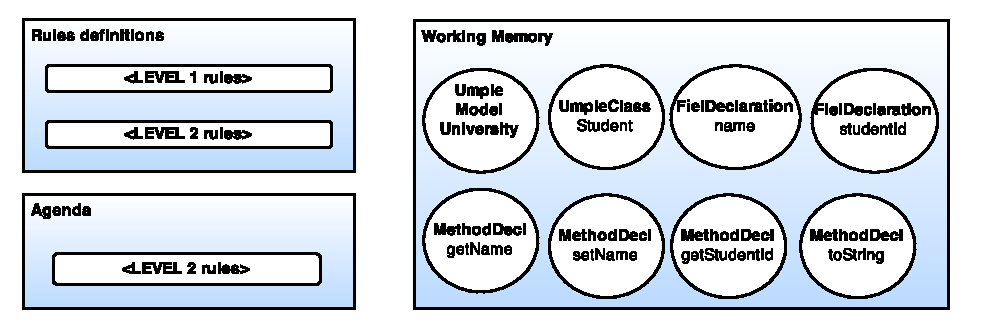
\includegraphics[width=0.98\textwidth]{Figures/ruleModel2.pdf}
\caption{Rule Engine snapshot after initial transformation}
\label{fig:ruleModel2}
\end{figure}

The rule engine then attempts to find objects matching the conditions in the rules. The only set of rules that can be matched to objects in the Working Memory are the rules related to attributes, since the only rules in the agenda are those for `LEVEL2' and the rules for `LEVEL1' have already been applied. In particular, the unique rule
that can be executed at this moment is the rule named \textit{`Field\_CanBeUmpleAttribute'} since all other rules require an instance of an Umple attribute in memory. As we have illustrated before in Figure \ref{fig:ruleModel2}, no instance of an Umple attribute exists or has been added so far. Rule \textit{`Field\_CanBeUmpleAttribute'} is presented in Listing \ref{lst:FieldCanBeUmpleAttribute}.

\begin{lstlisting}[language={drools},label=lst:FieldCanBeUmpleAttribute, caption=Rule  FieldCanBeUmpleAttribute]
rule "FieldCanBeUmpleAttribute"
agenda-group "LEVEL2" 
 when
	fieldDeclaration: FieldDeclaration()
	uClass: UmpleClass()
	method: MethodDeclaration()
	eval(isPrimitiveOrStringOrTime(fieldDeclaration))				   
	eval(uClass.getName()
	     .equals(getFieldCuATTontainerName(fieldDeclaration)))
	eval(uClass.getName().equals(getMethodContainerName(method)))
	eval(uClass.getAttribute(getFieldName(fieldDeclaration))== null)
	eval(hasFieldAGetter(method, fieldDeclaration, uClass.getName()))
 then 
	String attrName = getFieldName(fieldDeclaration);
	String attrType  = getAttributeType(fieldDeclaration);
	Attribute uAttr = 
	  new Attribute(attrName, attrType, null, null, false, uClass);
	uAttr.setModifier("settable");
	uClass.addAttribute(uAttr);
	removeClassField(fieldDeclaration, uClass);
	update(uClass);    	
	insert(uAttr);
end
\end{lstlisting}

The rule in Listing \ref{lst:FieldCanBeUmpleAttribute} creates an Umple attribute with information extracted from a field declaration. It does so if and only if the following conditions are met:
\begin{itemize}
\item In Lines 4,5,6. We require instances of a field, Umple class and method declarations in order to assess whether or not the field can become an Umple attribute of that class. These elements need to be found in the Working Memory. 

\item In Line 7. The field needs to be of a primitive type.

\item In Line 8-9. The field needs to be declared in the Class used to produce the current instance of the Umple Class.

\item In Line 10. The method declaration needs to be declared in the Class that derived the current instance of the Umple Class.

\item In Line 11. The Umple class must not possess an attribute with the name of the current instance of the field declaration. This is to avoid duplicates.

\item In Line 12. The field possesses a getter in the Class that derived the current instance of the the Umple Class.
\end{itemize}

If a field (and other model elements) matches the above conditions. A new Umple attribute is created with the information extracted from the instance of the field declaration and associate to the current instance of Umple Class (Line 16). The name (Line 14) and type (Line 15) are initialized as well. By default, our newly created Umple attribute is declared as settable (Line 17). The attribute is then added to a matched Umple Class (Line 18). The Helper function \textit{removeClassField} in Line 18 removes the field declaration from the extra code of the Umple Class since it has been refactored into an Umple attribute. Recall from the previous subsections that the field declaration was appended to the extra code of the Umple class. In Line 19, we updated the Umple class residing in the Working Memory. The clause `\textit{update}' is optional but we explicitly invoke it for logging purposes.

Finally, in Line 20, the attribute is put into the working memory so subsequent transformations can be made such as determining if the attribute is lazy or not. In fact, this Umple attribute as we will explain later, meets all conditions to be a `lazy' attribute. Lazy attributes have been introduced in Chapter 2. This process of matching objects with rules as we have described so far for this transformation step is summarized in Figure \ref{fig:ruleModel3}. As can be seen in the Figure, an instance of Umple attribute has been added to the Working Memory as a result of the match. Objects in yellow are the ones queried when evaluating the conditions of the rule. 

\begin{figure}[h]
\centering
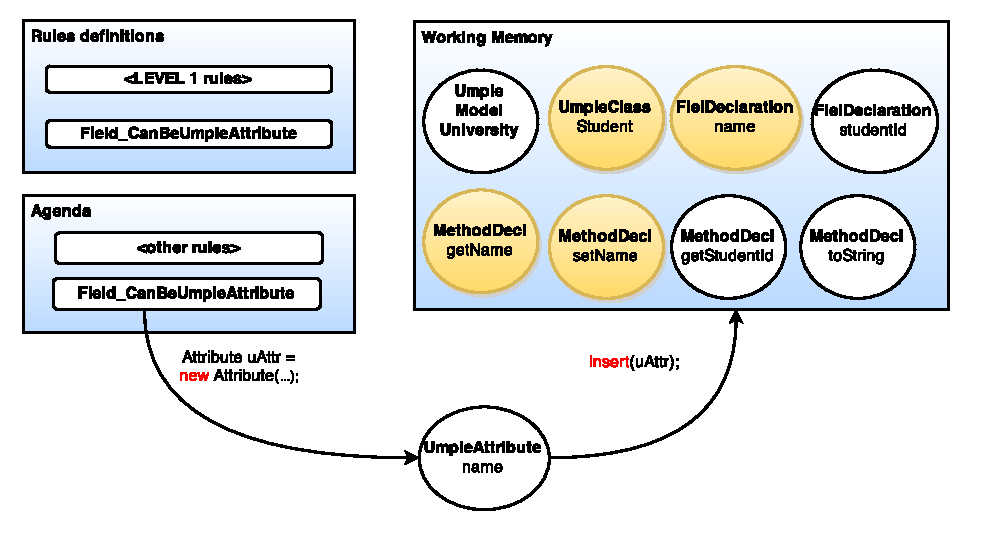
\includegraphics[width=0.98\textwidth]{Figures/ruleModel3.pdf}
\caption{Pattern matching and creation of an UmpleClass}
\label{fig:ruleModel3}
\end{figure}

We are not done yet since we need to remove or refactor the getters  and/or setters of the field (that became an attribute). For instance, if the rule (omitted) `\textit{hasFieldSimpleGetter}' or `\textit{hasFieldSimpleSetter}' is matched to any field previously transformed into an attribute, the method declaration is removed from the appended code of the Umple class. As is the case in our example, getName(), setName() and getStudentId() are removed from the `Student' Umple class.
When the field has a getter/setter that is not simple, an instance of the class CodeInjection (refer to Umple's metamodel) is created to take into account the code differing from the original getter/setter.

Finally, the rule named \textit{isLazyAttribute} in Listing \ref{lst:isLazyAttribute},  matches and converts any basic attribute (in memory) that conforms to the required conditions into a lazy attribute (e.g. attribute.setIsLazy(true)). These required conditions are listed next (Lines refer to Listing \ref{lst:isLazyAttribute}): 

\begin{itemize} 
\item In Lines 4,5,6. We require instances of a field, Umple class, method declaration and an Umple attribute in order to assess whether or not the attribute can become a lazy attribute. These elements need to be found in the Working Memory. 
\item In Line 8. The current instance of the Umple class needs to be the one owning the Umple attribute.
\item In Line 9. The field needs to be declared in the Class that derived the current instance of the Umple Class.
\item In Line 10. The method declaration needs to be declared in the Class that derived the current instance of the Umple Class.
\item In Line 11. A (double) check to ensure that the attribute belongs to the class.
\item In Line 12. The current instance of the field declaration is the one used to derive the current instance of the attribute.
\item In Line 13: The class in which the field is declared is NOT one of the constructor arguments. As per definition of a lazy attribute.
\end{itemize}

\begin{lstlisting}[language={drools},label=lst:isLazyAttribute, caption=Rule isLazyAttribute]
rule "isLazyAttribute"
agenda-group "LEVEL2" 
 salience 50
 when
  fieldDeclaration: FieldDeclaration()
  method: MethodDeclaration(method.isConstructor())
  attribute: Attribute(isLazy==false)
  uClass: UmpleClass(getAttributes().size() > 0 && 							      getAttributes().contains(attribute))
  eval(uClass.getName().equals(getFieldContainerName(fieldDeclaration)))
  eval(uClass.getName().equals(getMethodContainerName(method)))
  eval( attribute.getUmpleClass() == uClass) 
  eval( attribute.getName().equals(getFieldName(fieldDeclaration))) 
  eval(isFieldInContructor(method, fieldDeclaration, uClass.getName())==false);
  eval(getFieldName(fieldDeclaration).equals(attribute.getName()));
 then
  attribute.setIsLazy(true);
  update(attribute);
end
\end{lstlisting}

Since there are no more rules to execute, the rule engine stops. The updated Umple model is passed to the Generator for code generation. Note that the method \textit{toString()} is still part of the extra code of the Student Umple class.
The code generated by the \textit{Generator}, from the populated Umple model, is presented in Listing \ref{lst:level2exampleGenerator}. This concludes our second transformation step.

\begin{lstlisting}[style=umpleOut, label=lst:level2exampleGenerator, caption=Umple code generated -- Level 2]
namespace university.student;

class Student {
 depend java.util.Date;
	
 lazy String name;
 Integer studentId;
       
 public String toString() {
  return "The student " + getName() "has id=" + getStudentId();
 }
}   
\end{lstlisting}

\subsection{Automated Umplification of Associations}

As an example of the pattern matching for rules in Level 3 (associations), consider the code excerpt from Listings \ref{lst:exampleAutomated1} - \ref{lst:exampleAutomated2} . Assuming that the rules for the transformation of the classes, package declarations, import declarations and attributes have already been performed, we focus exclusively now on how the field declarations are transformed into Umple associations. In this particular example, we are expecting two Java field declarations to be transformed into association variables. Note that an Umple association is composed of two association ends. Each of the ends is represented by an association variable. In addition, take special note that the input code in this particular example is Umple code.

\begin{lstlisting}[style=UmpleIn,caption=Student.ump,label=lst:exampleAutomated1]
namespace university;

class Student { 
 Integer id; 
 lazy Boolean isActive; 
 immutable name; 
 const Integer MAX_PER_GROUP = 10; 
 after getName {
  if (name == null) { 
   throw new RuntimeException("Error");
  }
 }
  public Mentor mentor; 
  public Mentor getMentor() { 
   return mentor; 
  }
  public void setMentor(Mentor mentor) { 
   this.mentor = mentor; 
  } 
}
\end{lstlisting}

\begin{lstlisting}[style=UmpleIn,caption=Mentor.ump,label=lst:exampleAutomated2]
namespace university;
class Mentor { 

 depend java.util.Set;
 isA Person;
 
 Mentor() {}
 public Set<Student> students;
 public Set<Student> getStudents() {
  return students; 
 } 
 public void setStudents (Set<Student>students) { 
  this.students = students;
 } 
 public void addStudent( Student aStudent){
  students.add(aStudent); 
 }
 public void removeStudent(Student aStudent) {
  students.remove(aStudent);} 
 } 
 public String toString() {
      return(
         (name==null ? " " : name) + " " +
         students.size()+ " students"
      );
 }
}
\end{lstlisting}

The parser receives the source code from the mentioned listings, creates an Abstract Syntax Tree representation of it and transfers it to the Model Extractor. The Model Extractor uses the AST representation to create a Java model which is then traversed and decomposed into pieces by means of a Java class visitor. Table \ref{table:exampleTransformerAssocs} presents all the Java Elements collected by the Java visitor. An important fact that we have not revealed so far is that the parser is able to parse a sequence of \textit{independent} Java statements. As is required here, the Java parser will ignore the Umple code from the code excerpts in Listings \ref{lst:exampleAutomated1}-\ref{lst:exampleAutomated2} and will simply take into account the Java elements found. Contrary to what we have presented in the previous subsection (automated umplification of attributes), a TypeDeclaration will not be generated by the parser as shown in Table \ref{table:exampleTransformerAssocs}.

\begin{table}[h]
\caption{The input Java model elements produced}
\label{table:exampleTransformerAssocs}
\begin{tabular}{l|l}
\toprule
\rowcolor[HTML]{BBDAFF}
\textbf{ASTNode Type} & \textbf{Source Fragment}  \\ \midrule
\MyIndent \textbf{FieldDeclaration} &  "public Mentor mentor; "  \\ \hline
\MyIndent \textbf{MethodDeclaration} &  "public Mentor getMentor() {...}"  \\ \hline
\MyIndent \textbf{MethodDeclaration} &  "public void setMentor(Mentor mentor) {...}"  \\ \hline
\hline
\MyIndent \textbf{FieldDeclaration} &  "public Set \textless Student\textgreater students; "  \\ \hline
\MyIndent \textbf{MethodDeclaration} &  "public void setStudents (Set \textless Student \textgreater students) {}"  \\ \hline
\MyIndent \textbf{MethodDeclaration} &  "public void addStudent(...)"  \\ \hline
\MyIndent \textbf{MethodDeclaration} &  "public void removeStudent(..)"  \\ \bottomrule
\end{tabular}
\end{table}

The Transformer receives the Java model elements in Table \ref{table:exampleTransformerAssocs}, together with a newly created instance of an UmpleModel and places them into the Working Memory. 
At this point of time, as illustrated in Figure \ref{fig:ruleModelAssoc1}, the Working Memory contains the Umple model, two Umple Classes (Student and Mentor) and the Java model elements in Table \ref{table:exampleTransformerAssocs}. The Production Memory contains all the `LEVEL1', `LEVEL2' and `LEVEL3' rules and the Agenda only those from `LEVEL3' since the ones from `LEVEL1' and  `LEVEL2' have already been executed and removed from the stack. Objects with \textcolor{blue}{blue} border are those related to class \textcolor{blue}{Student} and those with \textcolor{red}{red} border are related to class \textcolor{red}{Mentor}. Depend and namespace declarations have been omitted here for brevity.

%Missing reference after 'elements in Table' above
% MG Fixed.
\begin{figure}[h]
\centering
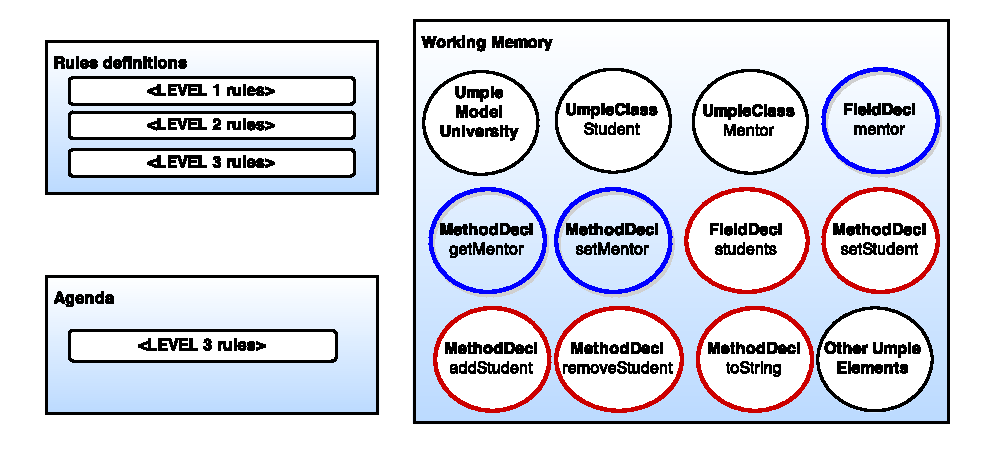
\includegraphics[width=0.98\textwidth]{Figures/ruleModelAssoc1.pdf}
\caption{Rule Engine snapshot before the automated umplification of associations}
\label{fig:ruleModelAssoc1}
\end{figure}

The rule engine then attempts to find objects matching the conditions in the rules. The only set of rules that can be matched to objects in the Working Memory are the rules related to associations (`LEVEL3'). In particular, the unique rule that can be executed at this moment is the rule named \textit{`FieldCanBeUmpleAssociation'} since all other rules require an instance of an Umple association in memory. As we have illustrated before in Figure \ref{fig:ruleModelAssoc1}, no instances of an Umple association or an association variable exist or have been added so far. Rule \textit{`Field\_CanBeUmpleAssociation'} is presented in Listing \ref{lst:FieldCanBeUmpleAssociation}. 

\begin{lstlisting}[language={drools},label=lst:FieldCanBeUmpleAssociation, caption=Rule FieldCanBeUmpleAssociation]
rule "Field_CanBeUmpleAssociation"
agenda-group "LEVEL3" 
no-loop
 when
  fieldDeclaration: FieldDeclaration()
  uClass: UmpleClass()
  method: MethodDeclaration()
  eval(!isPrimitiveOrStringOrTime(fieldDeclaration))				   
  eval(uClass.getName().equals(getFieldContainerName(fieldDeclaration)))
  eval(uClass.getName().equals(getMethodContainerName(method)))
  eval(uClass.getAssociationVariable(getFieldName(fieldDeclaration))== null)
 then
  String fieldType = getFieldType(fieldDeclaration);
  String fieldName = getFieldName(fieldDeclaration);
  AssociationVariable assocVar = new AssociationVariable(fieldName, fieldType,"", "", null, false);
  insert(assocVar); 	
end
\end{lstlisting}

The rule in Listing \ref{lst:FieldCanBeUmpleAssociation} creates an Association Variable with information extracted from a field declaration. It does so if and only if the following conditions are met:
\begin{itemize}
\item In Lines 5,6,7. We require instances of a field, Umple class and method declarations in order to assess whether or not the field can become an Umple association variable. These elements need to be found in the Working Memory. 

\item In Line 8. The field needs to be of a reference type. 

\item In Line 9. The field needs to be declared in the Class used to produce the current instance of the Umple Class.

\item In Line 10. The method declaration needs to be declared in the Class that derived the current instance of the Umple Class.

\item In Line 11. The Umple class must not already possess an association variable with the name of the current instance of the field declaration. This is to avoid duplicates.

\end{itemize}

If a field (and other model elements) matches the above conditions. A new Umple association variable is created with the information extracted from the instance of the field declaration (Line 14).

The class AssociationVariable has a single constructor which takes the following arguments:

\begin{enumerate}
\item String aName: corresponds to the rolename.
\item String aType: corresponds to the type declared.
\item String aModifier: defines the type of association (symmetric, reflexive). This argument is optional.
\item String aValue: correspond to the value provided as initialization (if any).
\item Multiplicity aMultiplicity: upper and lower bounds of the association variable.
\item boolean aIsNavigable: specifies if the association variable is navigable from the other association end.
\end{enumerate}

Also, it has other important fields used to refine certain characteristics of the variable (navigability, composition, etc.).

Finally, in Line 20, the association variable is put into the working memory so subsequent transformations can be made such as determining if the association variable can become part of an association. Given the fact that at this point we are not completely certain that this association variable will become an association end, the association variable is \textit{not} added to the current instance of the Umple class matched (i.e. `uClass.addAssociationVariable(assocVar)'). In our example, an association variable with name `mentor' of type `Mentor' has been created when matching elements of class `Student' and another one with name `students' of type `Student' when matching elements of class `Mentor'. Refer to rule  `MatchOtherAssociationEnd' which can be found in our main repository \cite{MappingRulesRepository}. 

We then attempt to determine whether the association variable is part of an association. Mutator and Accessor methods are analyzed at this point. This has been discussed in Chapter \ref{chap:detections}.
When the conditions are met, the association variable is added to the corresponding Umple class. Subsequent rules determine the multiplicity and navigability of the association ends. For instance, the lower bound of the multiplicity is obtained by analyzing the constructor and the upper bound by analyzing the field declaration itself. In our example, the multiplicity of our association variable `students' is determined as follows:

\begin{itemize}
\item Since the class possesses an empty constructor, so no instances of class Student are created when initializing an instance of class Mentor, the lower bound of multiplicity is `0'.
\item Since the field declares a collection of Student objects, the upper bound of multiplicity is `*' (many).
\end{itemize}

Once the multiplicity has been initialized for both association variables, an instance of an Umple association is created and added to \textit{only one} of the two Umple classes related. By default, if the association is bidirectional, we insert the association in the first Umple class retrieved from the Working Memory. In cases where the association is not navigable from both ends, the association is inserted in the class in which the association is visible.

We are not done yet since we need to remove or refactor the getters  and/or setters of the field (that became an association). In fact, the field declarations as well as the method declarations enumerated in Table \ref{table:exampleTransformerAssocs} are removed from the `extra code' of Umple classes `Mentor' and `Student', respectively. This is achieved by means of the helper functions `removeClassField(fieldDeclaration, uClass)' and `removeMethod(method, uClass)'. The `removeClassField(fieldDeclaration, uClass)' is presented in Listing \ref{lst:removeClassField}.

\begin{lstlisting}[style=java, label={lst:removeClassField}, caption=Function removeClassField]
public static  void removeClassField(FieldDeclaration field, UmpleClass uClass){
 String beforeExtraCode = uClass.getExtraCode();
 String toRemove = field.toString();
 String afterExtraCode = beforeExtraCode.replace(toRemove,"");
 // Clean extracode from class
 uClass.resetExtraCode();
 // Append new extraCode
 uClass.appendExtraCode(afterExtraCode);
}
\end{lstlisting}

Since there are no more rules to execute, the rule engine stops. The updated Umple model is passed to the \textit{Generator} for code generation. Note that the method \textit{toString()} is still part of the extra code of the Student Umple class. This concludes our third transformation step.

In the next section, we provide an overview of the tools currently available to support the umplification reverse-engineering process.

\section{Umplificator Tooling}

The Umplificator is available as an IDE and works within Eclipse; it also operates as a command-line tool to allow rapid bulk umplification and easier automated testing. Both tools are built and deployed using the Ant scripting language; resulting in several executable jars as well as for the Eclipse plugins. Table \ref{table:jars} describes the various jars deployed as part of our automated building process. In the table, X corresponds to the version, Y to the revision and Z to the build number. Our current version is `1.22.0.5146'.

\begin{table}[h]
\caption{Artifacts deployed during the building process of the Umplificator}
\label{table:jars}
\centering
\begin{tabular}{l|p{7cm}}
\toprule
\rowcolor[HTML]{BBDAFF}
\textbf{Name} & \textbf{Description}  \\ \midrule
cruise.umplificaror.eclipse\_vX.X.X.jar &  Plug-in for the Eclipse IDE 
\\ \hline
umplificator\_X.Y.Z.jar & Command-Line tool for umplification 
\\ \hline
validator\_X.Y.Z.jar & Command-Line tool that checks whether the input Umple code generates compilable base language code. 
\\ \bottomrule
\end{tabular}
\end{table}

Umplifying source code by means of the command-line tool can be done using the following command:

\vspace{\baselineskip}
\begin{lstlisting}[style=umplePlain]
< java -jar umplificator_1.21.0.4666.jar inputFile -level=0,1,2 
       -splitModel -dir -path >
\end{lstlisting}

where:
\begin{itemize}
\item \textbf{inputFile} can be an Umple file, base language file (.java, .cpp) or Source directory (containing java/Umple/cpp files).
\item \textbf{level}: can be 0,1,2 and corresponds to the refactoring that we want to achieve. 0 for the initial (classes, namespace, imports, etc.); 1 for the refactoring of attributes; 2 for the refactoring of associations. Level 2 includes transformations from level 0 and 1. Level 1 includes (and requires) transformations from level 0.
\item \textbf{splitModel} (optional): creates two files for each input file; one containing the modeling constructs, one containing the algorithmic and logic code (extra code). 
\item \textbf{dir} (optional): creates directories following the namespace structure.
\item \textbf{path}: the output directory name where the resulting Umple files will be located.
\end{itemize}

Additionally, the Umplificator is available as an online tool, called UmplificatorOnline. The tool is under development but will be deployed soon for public access. We have created this project for several purposes. Casual users are able to experiment with the latest version of the Umplificator with no more than a browser and an Internet connection. This allows curious developers to try out the tool. Figure \ref{fig:umpleonline} presents the initial page of the UmplificatorOnline.
An open-source project \textit{downloader} has been implemented as part of this Web tool. The tool runs the  Umplificator main Jar (umplificator\_1.21.0.4666.jar) for its reverse-engineering capabilities. An additional service (Scripts) to download projects from Github, SourceForge and GoogleCode to the local system with a specific directory structure has also been developed. This is further discussed in Chapter \ref{chap:evaluation}.

The preliminary release of the tool allows developers to:

\begin{itemize}
\item Select an Open-Source \textbf{repository}: The user can select projects from GoogleCode, SourceForge or GitHub.
\item Select an Open-Source \textbf{project} to umplify. The projects listed (in the second combo-box) have been automatically selected based on a number of predefined criteria. The criteria for project selection are that the project is marked as a small or medium-size system and that it is written in Java or C++.
\item Select the \textbf{level} of refactoring desired.
\item Select one of more \textbf{options}. The options have been described during our discussion of the command-line tool.
\end{itemize}

\begin{figure}[h]
\centering
\frame{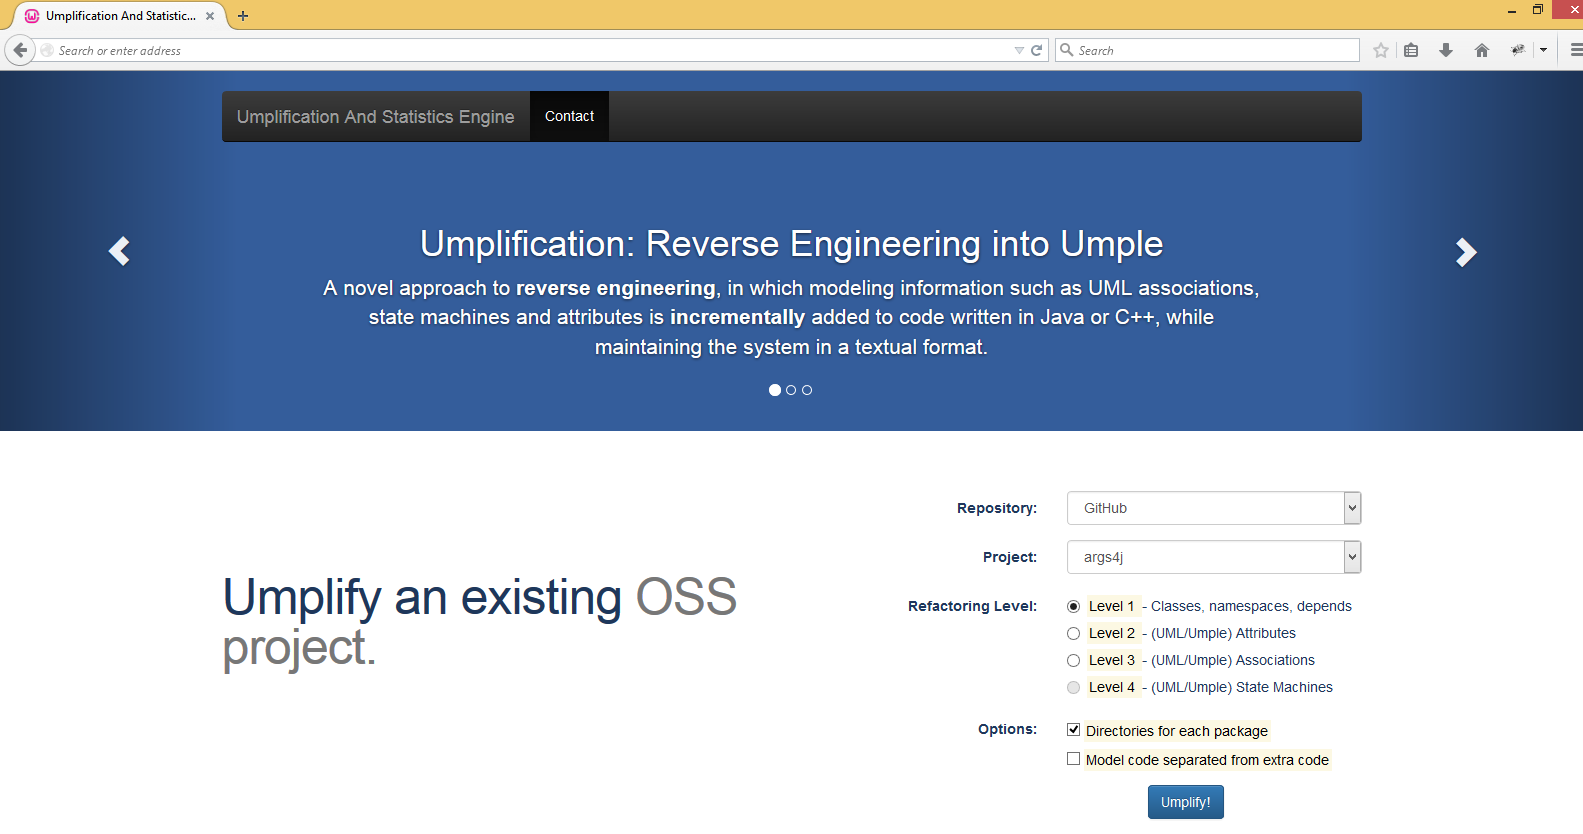
\includegraphics[width=0.98\textwidth]{Figures/UmplificatorOnline.png}}
\caption{The Umplificator online - A PHP Web application}
\label{fig:umpleonline}
\end{figure}


 % The Umplificator Technologies

\lhead{\emph{\leftmark}}  
\chapter{Evaluation}
\label{chap:evaluation}
% how far can we umplify a new system
In order to ensure that the results presented in this thesis are of high engineering quality and are as valid as possible from a scientific perspective, several approaches need to be followed. We validated our reverse engineering approach  by studying the application of our approach on various software systems. We adopted a \textbf{four-phase validation process} with the following steps:

\begin{description}

\item[Testing Phase]
Unit testing is carried out following a Test Driven Development approach (TDD).

\item[Pre-validation Phase]
Small Java systems written in high quality Java code, with known corresponding models, are employed to validate the accuracy of the transformations performed by the Umplificator.

\item[Initial Phase]
Medium and large  open-source projects are employed to validate the accuracy of the transformations and mapping rules. This set of open source projects will be known as the \textbf{`training set'}. The goal of this phase is to ensure the correctness and precision of the transformations on the training set.

\item[Machine Learning-Based Phase]
In this phase, we umplify a set of randomly selected systems, the \textbf{`testing set'} and assess the extent to which our transformations still work. We document the errors encountered during this phase of validation.

\end{description}

In general all four of the above phases are conducted in an iterative manner. In other words, we develop the Umplificator in small chunks that are validated at the same time.

This chapter is organized as follows: in the next sections we present each of the four phases of validation including the results obtained.  Finally, we provide extended details on the largest systems that were umplified during the four phases. 

\section{Testing Phase}
\label{sec:testingUmplificator}
As illustrated in Section \ref{chap:tool}, the Umplificator includes: a \textbf{parser}, a \textbf{model extractor}, a \textbf{transformer} and an Umple code \textbf{generator}. Each of the components is independently tested to ensure high quality as illustrated in Figure \ref{fig:testingPhase}. The testing phase explained in this section concerns only the testing process within the scope of the Umplificator.  In other words, we are testing the Umplificator implementation and \textbf{not} testing the set of possible umplified systems generated using our tool. 

At present there are over 135 tests that span all components of the tool (parser, extractor, transformer, generator) and are run as part of our automated building process.

In the subsequent sections we provide an overview of each aspect of the Umplificator's testing approach. 

\begin{figure}[h]
\centering
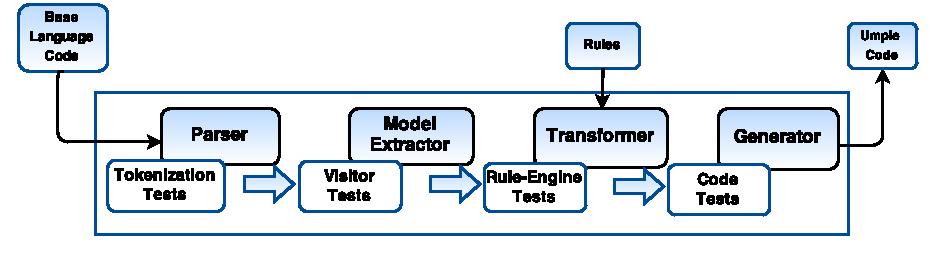
\includegraphics[width=1\textwidth]{Figures/testingPhase.pdf} 
\caption{Umplificator Testing Infrastructure}
\label{fig:testingPhase}
\end{figure}

\subsection{Testing the Base Language Code Parsers}

Testing the Umplificator parser is centered on the creation of the Abstract Syntax Tree (AST) from base language code. Our tests ensure that Base Language code is parsed and tokenized as we expect.

A simple parser test that verifies that the list of detailed problem reports (warnings, or compilation errors) noted by the compiler during the parsing or the type checking of the compilation unit (file) is what we expect, is shown in Listing \ref{lst:simpleFileWithTwoErrors}.
In this particular parser test, we are expecting two problems (compilation errors) since the input compilation unit contains two errors at two different locations in the code. The input code has been omitted. 

\begin{lstlisting}[style=java, label={lst:simpleFileWithTwoErrors}, caption=A Parser Test]
@Test
public void simpleFileWithTwoErrors()
{
  File testFile = new File(pathToInput+"SimpleFileWithTwoErrors.java");
  String code = SampleFileWriter.readContent(testFile);
  JavaParser javaParser = new JavaParser(); // JDT Parser
  CompilationUnit unit  = javaParser.parseUnit(code);
  Assert.assertEquals(2,unit.getProblems().length());
}
\end{lstlisting}

The pattern for parser-related test is presented in Listing \ref{lst:parserTestX}:

\begin{lstlisting}[style=java, label={lst:parserTestX}, caption=A pattern for parser tests]
@Test
public void parserTestX()
{
  // Step 1: Load external source file (Java or C++ file)
  // Step 2: Parse file (ensure parsing successful) 
  // Step 3: Verify tokenization
  // Step 4: Clean up
}
\end{lstlisting}

\subsection{Testing the Model Extractor}

Testing the model extractor ensures that from the tokens obtained through the parser we obtain a valid base language model representation (e.g. Java model, Umple model, CPP model). In particular, as we have implemented a visitor (software design pattern \cite{gamma1994design}) to traverse the different elements of the retrieved base language model, our tests certify that the visitor returns the desired number of elements.

For instance, if the test input file contains (Listing \ref{lst:inputVisitor}): 

\begin{lstlisting}[style=java, label={lst:inputVisitor}, caption=Java input file for test]
package cruise.umplificator.visitorTestFiles;

 import java.util.*;
 import java.io.*;

 @SuppressWarnings("unused")
 public class InputForVisitorTest { 

  boolean result = true;
  char capitalC = 'C';
  byte b = 100;
  short s = 10000;
  int i = 100000;
  double d1 = 123.4;
  long creditCardNumber = 1234_5678_9012_3456L;

  InputForVisitorTest () { }

  InputForVisitorTest(byte b) {
   this.b=b;
  }

  public int getB(){
   return b;
  }
}
\end{lstlisting}

in the unit test shown in Listing \ref{lst:JavaVisitorTest} we assert that the (Java) visitor returns: 7 field declarations (Lines 17-20), 2 import declarations (Lines 23-27), 3 method declarations (Lines 37-41) and a package name `cruise.umplificator.visitorTestFiles' (Line 30-34).


\begin{lstlisting}[style=java,label={lst:JavaVisitorTest}, caption=A JavaVisitorTest.java]
public class JavaVisitorTest {

String pathToInput;
JavaClassVisitor visitor ;
	
 @Before
 public void setUp() throws Exception {
  pathToInput = SampleFileWriter.rationalize("test/cruise/umplificator/visitorTestFiles/");
  File testFile = new File(pathToInput+"InputForVisitorTest.java");
  String code = SampleFileWriter.readContent(testFile);
  JavaParser javaParser = new JavaParser();
  CompilationUnit unit  = javaParser.parseUnit(code);
  visitor = javaParser.getJavaVisitor();
 }
	
 @Test
 public void field_declarations_returned_in_java_file()
 {
  Assert.assertEquals(7, visitor.numberOfFieldDeclarations());
 }
		
 @Test
 public void imports_returned()
 {
  int nbImports = visitor.numberOfImportDeclarations();
  Assert.assertEquals(2, nbImports);
 }
	
 @Test
 public void packages_returned()
 {
  String packageName = visitor.getPackageDeclaration().getName().getFullyQualifiedName();
  Assert.assertEquals("cruise.umplificator.visitorTestFiles", packageName);
 }

 @Test
 public void methods_returned()
 {
  int nbMethods = visitor.numberOfMethodDeclarations();
  Assert.assertEquals(3, nbMethods);
 }
\end{lstlisting}

\subsection{Testing the Transformer}

Testing the \textbf{transformer} involves ensuring that our Rule-Engine receives the input, fires the corresponding mapping rules and produces the expected output.
For instance, if the input of our tests below is the Java class presented in Listing \ref{lst:inputVisitor}, we expect all the assertions in the test class \textit{RulesAttributesTypesTest} to pass. The JUnit test class, as shown in Listing \ref{lst:testClassSetup}, contains a  method \textit{setUp()} that specifies the work to be done before running each test such as initializing instance variables. 

In Line 18 we parse the input file and create an Umple class that is inserted into the working memory of the Rule Engine. In Line 22, an Umple class is inserted into the Working memory (of Drools Rule Engine). Note that in Line 21  the desired \textbf{level of refactoring} includes Umple attributes (and excludes Umple associations) since the goal of this test class is to ensure the correct mapping between variables possessing certain characteristics and Umple attributes. Finally, we clean the working memory of the rule engine (Line 28).

\begin{lstlisting}[style=java, label=lst:testClassSetup, caption=RulesAttributesTypesTest class]
public class RulesAttributesTypesTest {

 String pathToInput;
 JavaClassVisitor visitor ;
 RuleRunner runner  = new RuleRunner();
 RuleService ruleService= new RuleService(runner);
 KieSession kieSession;
 UmpleClass uClass;
 CompilationUnit compilationUnit;
	
@Before
public void setUp() throws Exception {
 pathToInput = SampleFileWriter.rationalize("test/cruise/umplificator/visitorTestFiles/   InputForVisitorTest.java");
 File testFile = new File(pathToInput);
 String code = SampleFileWriter.readContent(testFile);
 visitor = new JavaClassVisitor();
 JavaParser javaParser = new JavaParser();
 javaParser.parseUnit(code);
 visitor = javaParser.getJavaVisitor();
 uClass = new UmpleClass("Test");
 kieSession = ruleService.startRuleEngine(RefactoringLevel.ATTRIBUTES);
 kieSession.insert(uClass);
}
 // test cases ...
 
 @After
 public void tearDown() throws Exception {
  runner.dispose();		
 }
}
\end{lstlisting}

The unit test \textit{testNumberOfObjectsInWorkingMemory} in Listing \ref{lst:testNumberOfObjectsInWorkingMemory} ensures that at this point of time, there is only one element in the working memory (the Umple class inserted  before) since the mapping rules have not been fired yet.

\begin{lstlisting}[style=java, label=lst:testNumberOfObjectsInWorkingMemory, caption=Test asserting the working memory contents]
 @Test
 public void testNumberOfObjectsInWorkingMemory() {
   Assert.assertEquals(1, kieSession.getObjects().size());
 }
\end{lstlisting}

The unit test \textit{testCorrectMappingBetweenPrimitiveField2UmpleAttribute} in Listing \ref{lst:testCorrectMappingBetweenPrimitiveField2UmpleAttribute} validates the mappings between the Java fields (input) and the Umple attributes. 
\begin{lstlisting}[style=java, label=lst:testCorrectMappingBetweenPrimitiveField2UmpleAttribute, caption=Test asserting mappings of fields and attributes]
@Test
public void testCorrectMappingBetweenPrimitiveField2UmpleAttribute() {
 // Insert facts into knowledge base
 for(FieldDeclaration field: visitor.getFieldDeclarations()){
  kieSession.insert(field);
 }
 // Fire rules
 kieSession.fireAllRules();
 // Is not Null
 Assert.assertNotNull( uClass.getAttribute(0));
 Assert.assertNotNull( uClass.getAttribute(1));
 Assert.assertNotNull( uClass.getAttribute(2));
 Assert.assertNotNull( uClass.getAttribute(3));
 Assert.assertNotNull( uClass.getAttribute(4));
 Assert.assertNotNull( uClass.getAttribute(5));
 Assert.assertNotNull( uClass.getAttribute(6));

 // Type has been set correctly
 Assert.assertEquals("Boolean", uClass.getAttribute(0).getType());
 Assert.assertEquals("String", uClass.getAttribute(1).getType());
 Assert.assertEquals("Integer", uClass.getAttribute(2).getType());
 Assert.assertEquals("Integer", uClass.getAttribute(3).getType());
 Assert.assertEquals("Integer", uClass.getAttribute(4).getType());
 Assert.assertEquals("Double", uClass.getAttribute(5).getType());
 Assert.assertEquals("Double", uClass.getAttribute(6).getType());
 // Name has been correctly set
 Assert.assertEquals("result", uClass.getAttribute(0).getName());
 Assert.assertEquals("capitalC", uClass.getAttribute(1).getName());
 Assert.assertEquals("b", uClass.getAttribute(2).getName());
 Assert.assertEquals("s", uClass.getAttribute(3).getName());
 Assert.assertEquals("i", uClass.getAttribute(4).getName());
 Assert.assertEquals("d1", uClass.getAttribute(5).getName());
 Assert.assertEquals("creditCardNumber", uClass.getAttribute(6).getName());
}
\end{lstlisting}
The following gives details of Listing \ref{lst:testCorrectMappingBetweenPrimitiveField2UmpleAttribute}:
\begin{itemize}
\item In Lines 4-6 the fields declarations of the Java class are inserted into the Working Memory.
\item The mapping rules are fired in Line 8. 
\item Line 10-16: We assert that the Rule Engine has correctly mapped the field declarations into Umple attributes. The Umple class must now contain 6 attributes. 
\item In Lines 19-28 and 27-33, we assert that the name and type of the field declaration has been correctly assigned to the Umple attribute.
\end{itemize}

The unit test \textit{testCorrectMappingBetweenImport2Depend} in Listing\ref{lst:testCorrectMappingBetweenImport2Depend} also ensures the correct mapping between the input Java import declarations and the Umple depends clause.

\begin{lstlisting}[style=java, label=lst:testCorrectMappingBetweenImport2Depend, caption=Test asserting mappings of imports and depends]
@Test
public void testCorrectMappingBetweenImport2Depend() {
for(ImportDeclaration importDecl: visitor.getImportDeclarations()){
 kieSession.insert(importDecl);
}
kieSession.fireAllRules();
 Assert.assertEquals(2, uClass.getDepends().size());
 Assert.assertEquals("java.util.*",uClass.getDepends().get(0).getName());
 Assert.assertEquals("java.io.*",uClass.getDepends().get(1).getName());
}
\end{lstlisting}

\subsection{Testing the Umple Code Generator}

Testing the code generator involves asserting that from an input file we obtain the expected Umple file. Briefly, we compare the content of an Umple file as generated by the Umplificator and the expected Umple file. 

\begin{lstlisting}[style=java, label=lst:JavaToUmpleVariablesToAttributes003, caption=A code generator test]
@Test
public void JavaToUmple_VariablesToAttributes_003(){
 String fileName = "003_JavaToUmple_VariablesToAttributes";
 File javaFile = new File(pathToRoot+fileName+"_java.java"); //INPUT
 File umpleFile = new File(pathToRoot+fileName+"_umple.ump"); //OUTPUT
 // Umplify file. Process must succeed!
 assertTrue(umplificator.umplifyElement(javaFile));
 // Get the output content
 assertOuputAndFile(umpleFile);
 // Clean files 
 filesToDelete.add(fileName);
}
// Helper Functions
public void assertOuputAndFile(File expectedContentFile)
{
try {
 String inputFileContent = FileUtils.readFileToString(expectedContentFile);
 String outputModel  = umplificator.getOutputModel().getCode();
 assertEquals(inputFileContent, outputModel);
 } catch (IOException e) { fail();}
}
\end{lstlisting}

The test in Listing \ref{lst:JavaToUmpleVariablesToAttributes003}, performs the umplification process on the Java input file, and compares the content of the code produced by the Umplificator with the code of the expected Umple file. The comparison is done with the help of method \textit{assertOuputAndFile}.

Testing the different components of our infrastructure allows for better defect management by representing bugs as failing tests, effectively diminishing the time and effort required to localize any defects that might occur. In other words, this multi-level testing helps to make sure that a change or addition of a new feature doesn't break any existing functionality and if there is any bug to quickly locate the defective component. When a defect is uncovered, it might be one of the following:

\begin{enumerate}
\item Defect in the way the base language code is tokenized and converted into an abstract syntax tree.

\item Incorrect population of the base language metamodel instance from the tokenized language.

\item Inappropriate behavior of the rule engine.

\item Syntax errors in the generated Umple code.

\item Semantic errors in the generated base language code (from the umplified model).
\end{enumerate}

\section{Pre-Validation Phase}

We have tested the umplificator using our own repository of 42 small Umple examples. This collection of models covers a wide variety of domains ranging from Banking to Warehouse control, and is available for review online \cite{umpleexamples}.

We generated Java code from these examples using the Umple compiler, and then used the Umplificator to re-generate Umple models for each example. The process is illustrated in Figure \ref{fig:preValidation}. The goal of this pre-validation phase is to confirm that each original Umple model is regenerated correctly; in other words that it is semantically identical to the \textit{UmpleModel'}  generated by the Umplificator.
 
\begin{figure}[h]
\centering
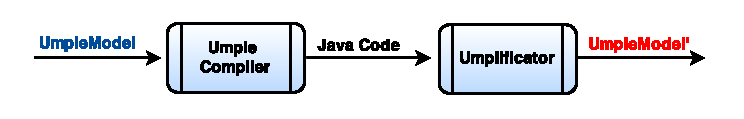
\includegraphics{Figures/preValidation.pdf} 
\caption{The pre-Validation phase: Comparing UmpleModel and UmpleModel'}
\label{fig:preValidation}
\end{figure}

Table \ref{table:umpleexamples} lists the Umple examples used in this pre-validation phase, as well as  some statistics about them (number of lines of code of the Umple model, the number of lines of code of the corresponding Java system and the number of Java classes).

\begin{table}
\caption{Small examples used for first phase of validation}
\label{table:umpleexamples}
\centering
\begin{tabular}{p{6cm}|rrr}
\toprule
\rowcolor[HTML]{BBDAFF}
\textbf{Name} & \textbf{\#Umple LOC} & \textbf{\#Java LOC} & \textbf{\#  Files} \\ \midrule
2DShapes & 44 & 509 & 9\\ \hline
AccessControl & 67 & 1560 & 6\\ \hline
Accidents & 42 & 730 & 4\\ \hline
Accommodations & 102 & 2215 & 9\\ \hline
AfghanRainDesign & 132 & 2610 & 13\\ \hline
Airline & 51 & 1800 & 8\\ \hline
Banking System A & 87 & 2400 & 13\\ \hline
Banking System B & 74 & 1650 & 12\\ \hline
Canal System & 69 & 2222 & 14\\ \hline
Decisions & 148 & 4153 & 15\\ \hline
Card Games (Oh Hell and Whist) & 134 & 2051 & 8\\ \hline
Claim (Insurance) & 19 & 408 & 2\\ \hline
Community Association & 68 & 1591 & 9\\ \hline
Co-op Education System & 69 & 2420 & 10\\ \hline
DMM Overview & 59 & 1165 & 10\\ \hline
DMM Source Object Hierarchy & 91 & 1774 & 16\\ \hline
DMM Relationship Hierarchy & 135 & 1119 & 31\\ \hline
DMM CTF & 93 & 932 & 4\\ \hline
Election System & 83 & 2875 & 11\\ \hline
Elevator System A & 42 & 1307 & 4\\ \hline
Elevator System B & 56 & 1971 &11\\ \hline
Genealogy A & 29 & 670 & 2\\ \hline
Genealogy B & 32 & 945 & 2\\ \hline
Genealogy C & 36 & 1017 & 3\\ \hline
Geographical Information System & 52 & 1174 & 11\\ \hline
Hospital & 65 & 1923 & 9\\ \hline
Hotel & 47 & 1888 & 10\\ \hline
Insurance & 63 & 1417 & 10\\ \hline
Inventory Management & 44 & 1753 & 7\\ \hline
Library & 42 & 1595 & 10\\ \hline
Mail Order System- Client Order & 38 & 1895 & 8\\ \hline
Manufacturing Plant Controller & 84 & 3089 & 11\\ \hline
Pizza System & 67 & 1555 & 9 \\ \hline
Police System & 64 & 3186 & 10\\ \hline
Political Entities & 32 & 842 & 5\\ \hline
Real Estate & 79 & 2071 & 8\\ \hline
Routes and Locations & 127 & 2089 & 9\\ \hline
School & 18 & 397 & 9\\ \hline
TelephoneSystem & 38 & 1838 & 7\\ \hline
University System & 32 & 1206 & 4\\ \hline
Vending Machine & 97 & 1696 & 8\\ \hline
WarehouseSystem & 83 & 2831 & 12\\ \hline
\bottomrule
\end{tabular}
\end{table}

For instance, the \textit{`Access Control Example'}, representing a system for managing access to facilities, is comprised of 6 classes, 8 associations, and 10 attributes. The Umple model is presented in Listing \ref{lst:accessControlEx} together with corresponding visual representation, a UML class diagram generated using our online tool (Figure \ref{fig:accessControlExample}). The unit test comparing the input umple model and the umplified model is shown in Listing \ref{lst:acsExample}.

\begin{lstlisting}[style=umpleIn,caption=Umple model for an access control System, label=lst:accessControlEx]
namespace access_control;

class FacilityType
{
  code;
  description { Menu, Record, Screen }
  key {code}
}

//Functional_Area
class FunctionalArea
{
  String code;
  0..1 parent -- * FunctionalArea child;
  description { Hr, Finance }
  key {code}  
}

//Facility_Functional_Area
association
{
  * FunctionalArea -- * Facility;
}

class Facility
{
  Integer id;
  lazy Time t; 
  * -> 0..1 FacilityType;
  Integer access_count;
  name;
  description;
  other_details;
  
  key {id}
}

class Role
{
  code;
  role_description { Dba, ProjectMgr }
  
  key {code}
}

class User
{
  Integer id;
  * -> 0..1 Role;
  first_name;
  last_name;
  password;
  other_details;
  key {id}
}

associationClass RoleFacilityAccessRight
{
  * Facility;
  * Role;
  CRUD_Value { R, RW }
}
\end{lstlisting}
%http://yuml.me/4aab4a38
\begin{figure}[h]
\centering
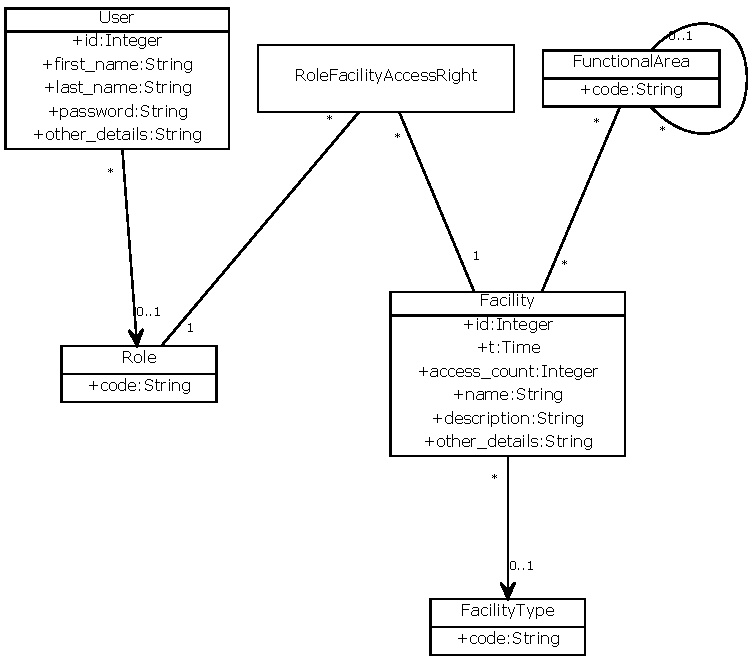
\includegraphics{Figures/accessControl.pdf} 
\caption{UML Class diagram of the Access Control system}
\label{fig:accessControlExample}
\end{figure}

\begin{lstlisting}[style=java,label={lst:acsExample},caption=Unit test to assert the access control example.]
@Test
public void AccessControlExample(){
 String folderName = "AccessControl";
 File inputFile = new File(pathToRoot+ File.separator +folderName +".ump");
 UmpleFile inputUmpleFile = new UmpleFile(inputFile);
 // Umplify all the files in folder
 List<File> inputFiles = FileHelper.getListOfFilesFromPath(pathToRoot+ File.separator +       folderName, new ArrayList<File>());
 // Umplify files. Process must succeed!
 assertTrue(umplificator.umplify(inputFiles));
 // This is the actual model, the one umplified 
 UmpleModel umplifiedModel = umplificator.getOutputModel();
 UmpleModel expectedModel = new UmpleModel(inputUmpleFile);
 expectedModel.run();		
 //1. Class FacilityType
 UmpleClass facilityTypeA = umplifiedModel.getUmpleClass("FacilityType");
 UmpleClass facilityTypeE = expectedModel.getUmpleClass("FacilityType");		
 Assert.assertEquals(1, facilityTypeA.numberOfAttributes());
 Attribute lazyAttributeA = facilityTypeA.getAttribute("code");
 Attribute lazyAttributeE = facilityTypeE.getAttribute("code");	
 assertEquals(lazyAttributeA.getIsLazy(),lazyAttributeE.getIsLazy());
 assertEquals(lazyAttributeA.getType(),lazyAttributeE.getType());		
 // 2. Class User
 UmpleClass userA = umplifiedModel.getUmpleClass("User");
 UmpleClass userE = expectedModel.getUmpleClass("User");	
 Attribute id = userA.getAttribute("id");
 Attribute firstname = userA.getAttribute("first_name");
 Attribute lastname = userA.getAttribute("last_name");
 Attribute other_details = userA.getAttribute("other_details");
 Attribute password = userA.getAttribute("password");
		
 Assert.assertEquals(userA.numberOfAttributes(), userE.numberOfAttributes());
 Assert.assertEquals("Integer", id.getType());
 Assert.assertEquals("String", firstname.getType());
 Assert.assertEquals("String", lastname.getType());
 Assert.assertEquals("String", other_details.getType());
 Assert.assertEquals("String", password.getType());
 // 3. Facility Class
 UmpleClass facilityA = umplifiedModel.getUmpleClass("Facility");
 UmpleClass facilityE = expectedModel.getUmpleClass("Facility");
 Assert.assertEquals(facilityA.numberOfAttributes(), facilityE.numberOfAttributes());

 Attribute timeAttr = facilityA.getAttribute("t");
 Attribute idAttr = facilityA.getAttribute("id");
 Attribute accessAttr = facilityA.getAttribute("access_count");
 Attribute nameAttr = facilityA.getAttribute("name");
 Attribute descAttr = facilityA.getAttribute("description");
 Attribute otherAttr = facilityA.getAttribute("other_details");
		
 Assert.assertTrue(timeAttr.isIsLazy());
 Assert.assertFalse(idAttr.isIsLazy());
 Assert.assertFalse(accessAttr.isIsLazy());
 Assert.assertFalse(nameAttr.isIsLazy());
 Assert.assertFalse(descAttr.isIsLazy());
 Assert.assertFalse(otherAttr.isIsLazy());
 // Compare both models, generally
 assertTrue(areModelsEqual(umplifiedModel,expectedModel));
}
\end{lstlisting}

In the test case above, the level of refactoring includes only attributes (Umple associations have not been extracted) so we are interested in the classes, generalizations and the attributes of each class. We assert that the classes have been correctly detected and that the attributes in each class have been correctly extracted (attribute type, attribute name and additional features). For instance, in Line 49 we assert that the attributes is \textbf{lazy}, since the variable is not one of the parameters in the constructor of the Java class \textit{Facility} (Java code is not shown here).

This pre-validation essentially demonstrates with a high level of confidence that the Umplificator works, at a basic level on a significant amount of Java code, but with a known and consistent structure. It was fairly easy to tailor our transformation rules to reverse-engineer code that we had generated ourselves. We know exactly what the structure of this code is; we know that it will be the same throughout each example, and we know that it will not change over time (or if it does change, at least we have control of both forward and reverse engineering). Pre-validation, says nothing about whether the Umplificator can work `in the wild', against unknown code. That is what we have to do in the next stages of validation.

Our pre-validation is similar to the concept of `dogfooding' \cite{ash2003web}, in that we are testing the Umplificator on our own code. But it is not `full' dogfooding since we have not yet attempted to convert the whole of the Umple compiler back from generated Java to Umple; the Umple compiler is very large and has a number of complexities that will make this a challenge we leave to future work.


\section{Initial Phase of Validation}

Our next step was to apply the Umplificator to various open-source systems written in Java. We use freely available systems to facilitate comparisons and replications of our evaluation. We provide some information on these systems in Table \ref{table:umplifiedSystems} including their version, number of lines of code and the number of classes.

Furthermore, we perform `\textit{manual}' umplification on all open-source systems in Table \ref{table:umplifiedSystems}. The results of the manual umplification are then compared to the results of our '\textit{automated}' umplification. 

We call this phase the `Initial' phase of validation because this is the first phase where we show that the Umplificator can work on systems that we have not created ourselves.

\begin{table}
\caption{Open-source systems umplified}
\label{table:umplifiedSystems}
\centering
\begin{tabular}{l|lrr}
\toprule
\rowcolor[HTML]{BBDAFF}
\textbf{Name} & \textbf{Version} & \textbf{LOC} & \textbf{\# of Classes} \\ \midrule
 1. JHotDraw \cite{jhotdraw}                   & 7.5.1   & 82132   & 694      \\ 
\hline 2.  Weka \cite{wekasvn}      & 3.7.13  & 278642  & 1370        \\ 
\hline  3. Java Bug Reporting Tool\cite{jbrtsvn} 		& 1.0     & 2629    & 27        \\ 
\hline  4. JEdit\cite{jeditsvn}                   	& 1.12    & 59699   & 84         \\ 
\hline  5. FreeMaker\cite{freemakersvn}               & 2.3.15  & 39864   & 131         \\ 
\hline  6. Java Financial Library\cite{jflsvn}  		& 1.6.1   & 1248    & 28          \\ 
\hline  7. Args4j\cite{args4jsvn}                 	 & 2.0.30  & 2223    & 61            \\
\bottomrule
\end{tabular}
\end{table}

More concisely, for each system studied, we have followed these steps:

\begin{enumerate}
\item We apply the different transformation steps on the input object-oriented system.

\item We run the test suite available for the system to ensure that code compiles and is semantically identical to the original input source code.

\item We run a custom-made code analyzer on the Umple system generated (umplified) to obtain the statistics of the detected (extracted) Umple constructs (attributes, associations). At this stage, we obtain the number of attributes extracted for each class, their type, as well as the number of all different types of associations.	

\item We compare our results with data obtained from manual umplification. That is, we umplify the system without the help of the Umplificator tool. The manual 	umplification, a very time consuming task, is usually performed by another software engineer (undergraduate students contributing to the Umple project). 

\item We compute the \textit{precision} and \textit{recall} of the results previously obtained. Precision assesses the proportion of the constructs (attributes, associations) identified that are valid -- in other words that were also identified by the manual umplification. Recall assesses the proportion of the independently-identified constructs that are found by our approach (a number near 1 would mean very few are missed by our detection algorithms). 

\item We refine our mapping rules to improve the precision of our algorithms. This step mainly concerns tuning the Umplificator. In general, tuning the Umplificator to increase its accuracy includes one or more of the following manual steps:

	\begin{enumerate}
		\item If there is an Umple construct that was missed from the extraction (false negative), we may add a new mapping rule to cover this case.
		
		\item If there is an Umple construct that was incorrectly identified (false positive), we may edit the corresponding mapping rule.
		\item If one of the methods requiring additional transformations (as described in Table \ref{table:transformations}) was incorrectly refactored, we may review and correct the refactoring action (a function in the Drools language) that led to the incorrect piece of code.

	\end{enumerate}
Briefly, the complexity of the tuning our tool depends on the number of false positives and false negatives that the tool generates. 
\end{enumerate}

The following are the definitions we have employed for the precision and recall measures \cite{precisionRecallDef}:

\[  Precision=\frac{|TP|}{|TP \cap FP|}\]
and \\
\[  Recall=\frac{|TP|}{|TP \cap FN|}\]

Where,
\begin{enumerate}
\label{sec:tuning}
\item \textbf{TP} is the number of true positives. They correspond to modeling construct that were correctly identified by our algorithms.
\item \textbf{FN} is the number of false negatives.  In the context of this work, they correspond to constructs that were missed from the automated umplification. 
\item \textbf{FP} is the number of false positives. They correspond to modeling constructs that were misidentified (false alarms). 
\end{enumerate}

The next sub-section presents the results of this validation stage. Specifically, we will present the statistics on the number of Umple constructs recovered from the various open-source projects in \ref{table:umplifiedSystems} as well as the \textit{precision} and \textit{recall} measures. It is important to recall at this point that the resulting output artifact from manual umplification and automated umplification is in both cases an Umple model. We run our code analyzer on the resulting umple model to get statistics and the information required for our comparisons. For instance, if we run the code analyzer on two (fictitious) models, one being the result of manual umplification (\textit{ManualModel}) and the other one the result of automated umplification (\textit{AutomatedModel}) of the same input system and we obtain the following results:

For \textit{ManualModel}:
\begin{enumerate}
\item ManualModel contains 1 class = \{A\}
\item Class A contains 3 attributes = \{a,b,c\}
\end{enumerate}

For \textit{AutomatedModel}:
\begin{enumerate}
\item AutomatedModel contains 1 class = \{A\}
\item Class A contains 3 attributes = \{a,b,d\}
\end{enumerate}

We can then compute the precision and recall measures. In our fictitious example above, the results are as follows:

\begin{enumerate}
\item True positives: 2 relevant attributes were correctly retrieved \{a,b\}
\item False negatives:  1 attribute was missed \{c\}
\item False positives: 1 attribute was incorrectly retrieved \{d\}
\end{enumerate}

The precision and recall for the recovery of attributes for our fictitious sample system is:


\begin{enumerate}
\item \textbf{Precision}: TP / (TP + FP) = 2 / (2 + 1) = 66.7\%
\item \textbf{Recall}: TP / (TP + FN) =  2 / (2 + 1) = 66.7\%
\end{enumerate}

Finally, the code analyzer mentioned before is an Umple feature that can be run on the command line:

\vspace{\baselineskip}
\begin{lstlisting}[style=umplePlain]
   java -jar umple.jar -g CodeAnalysis Test.ump
\end{lstlisting}
or using our online tool as shown in Figure \ref{fig:onlineCodeAnalyzer}.

\begin{figure}[h]
\centering
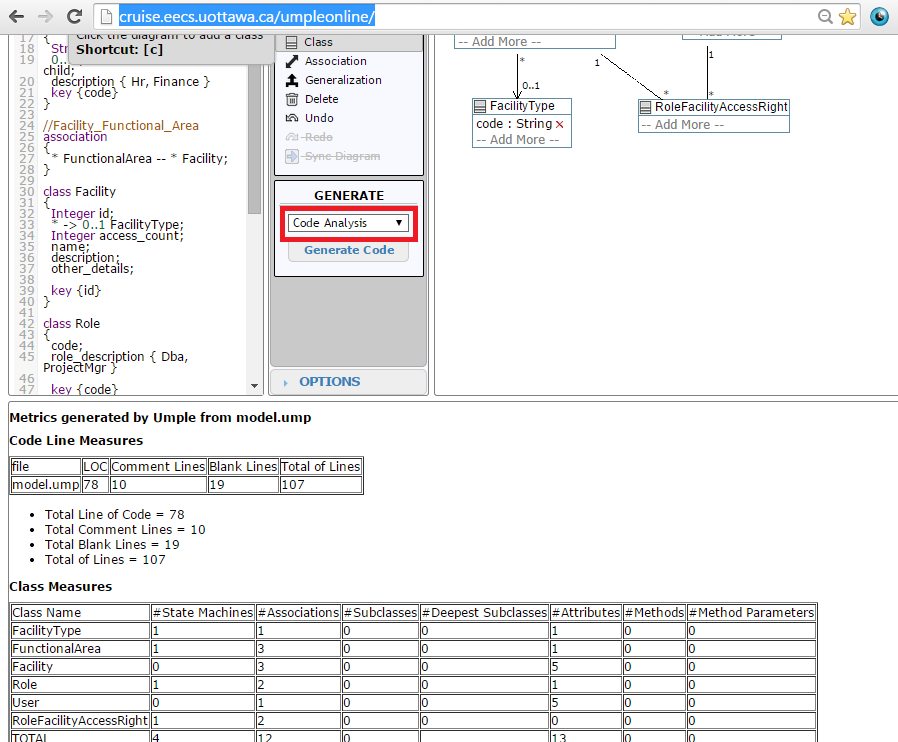
\includegraphics[width=0.75\textwidth]{Figures/UmpleOnlineCodeAnalyzer.png} 
\caption{Umple online - Code Analysis generation}
\label{fig:onlineCodeAnalyzer}
\end{figure}

\subsection{Results}

In the following tables, we will present the number of initially recovered  attributes, and associations (of each type) for each of the systems studied. Nine different types of associations were identified in previous work \cite{UmpleAssociations}; we present results for three of them, corresponding to the top multiplicity patterns in industry: optional-one-to-many, optional-one-to-one and many-to-many associations.

The results below are a snapshot following the first attempt at automated umplification on these systems. That is, no tuning had been performed on the Umplificator to improve the results. Since then, after tuning the Umplificator,  the precision and recall measures for all open-source systems studied in Table \ref{table:umplifiedSystems} has been increased to 100\%.

Tables \ref{table:umplifiedResultsSystems1} - \ref{table:umplifiedResultsSystems7} detail the number of generalizations, the number of attributes and the different types of associations for the systems studied.

The second column of Tables \ref{table:umplifiedResultsSystems1} - \ref{table:umplifiedResultsSystems7} presents the number of Umple constructs that were correctly recovered (True Positives). The third column presents the number of Umple constructs that were incorrectly recovered (False Positives). The fourth column presents the number of expected Umple constructs (True Positives + False Negatives, resulting from manual umplification). The last two columns present the precision and recall computations. Note that the number of missed Umple constructs (False Negatives) can be computed by subtracting the number of correctly retrieved Umple constructs from the number of expected Umple constructs. 


Let us look specifically at one of the tables, Table \ref{table:umplifiedResultsSystems1}; this shows the results of detection of Umple constructs for the JHotDraw framework.  It shows that for JHotdraw, 383 of the attributes were recovered; however only 95\% were actual attributes. It turns out that, 20 1-to-1 associations were mistakenly extracted as attributes. More details concerning the Umplification of JHotdraw and Weka will be given in Section \ref{sec:6CaseStudies}.

\begin{table}[h]
\caption{Results of umplification for JHotDraw}
\label{table:umplifiedResultsSystems1}
\centering 
\begin{tabular}{p{4cm}|rrrrr}
\toprule
\rowcolor[HTML]{BBDAFF}
\textbf{} & \textbf{TP}  & \textbf{FP} & \textbf{Expected} & \textbf{Precision}  & \textbf{Recall}\\ \hline
Attributes & 383  & 20  & 363  & 95\% & 100\% \\ \hline
Associations optional-one-to-many &  22 & 0 & 49 & 100\% & 45\% \\ \hline
Associations optional-one-to-one &  115 & 0 & 185  & 100\% & 62.2\% \\ \hline
Associations many-to-many & 30 & 0 & 32 & 100\% & 93.8\%\\ \bottomrule
\end{tabular}
\end{table}

\begin{table}[h]
\caption{Results of umplification for Weka}
\label{table:umplifiedResultsSystems2}
\centering 
\begin{tabular}{p{4cm}|rrrrr}
\toprule
\rowcolor[HTML]{BBDAFF}
\textbf{} & \textbf{TP}  & \textbf{FP}  & \textbf{Expected} & \textbf{Precision}  & \textbf{Recall}\\ \hline
Attributes & 1281	& 0	& 1510 & 100\%	& 84.9\% \\ \hline
Associations optional-one-to-many &  168 & 0 & 442 & 100\% & 38\% \\ \hline
Associations optional-one-to-one &  224 & 12 & 285 & 94.92\%  & 86.8\% \\ \hline
Associations many-to-many & 89 & 0 & 115 & 100\% & 77.4\% \\ \bottomrule
\end{tabular}
\end{table}

\begin{table}[h]
\caption{Results of umplification for the Java bug reporting tool}
\label{table:umplifiedResultsSystems3}
\centering 
\begin{tabular}{p{4cm}|rrrrr}
\toprule
\rowcolor[HTML]{BBDAFF}
\textbf{} & \textbf{TP}  & \textbf{FP}  & \textbf{Expected} & \textbf{Precision}  & \textbf{Recall}\\ \hline
Attributes & 31 & 0  & 31  & 100\% & 100\% \\ \hline
Associations optional-one-to-many &  9 & 0 & 12  & 100\%& 75\% \\\hline
Associations optional-one-to-one &  4  & 0 & 4  & 100\% & 100\% \\ \hline
Associations many-to-many & 7 & 0 & 7 & 100\% & 100\%\\ \bottomrule
\end{tabular}
\end{table}

\begin{table}[h]
\caption{Results of umplification for JEdit}
\label{table:umplifiedResultsSystems4}
\centering 
\begin{tabular}{p{4cm}|rrrrr}
\toprule
\rowcolor[HTML]{BBDAFF}
\textbf{} & \textbf{TP}  & \textbf{FP}  & \textbf{Expected} & \textbf{Precision}  & \textbf{Recall}\\ \hline
Attributes & 30  & 1 & 30 & 96.8\% & 100\%\\ \hline
Associations optional-one-to-many & 15  & 0 & 15  & 100\% & 100\% \\ \hline
Associations optional-one-to-one  &  22 & 0 & 22 & 100\% & 100\% \\\hline
Associations many-to-many &  40 & 0 & 48  & 100\% & 83.3\% \\ \bottomrule
\end{tabular}
\end{table}

\begin{table}[h]
\caption{Results of umplification for FreeMaker}
\label{table:umplifiedResultsSystems5}
\centering 
\begin{tabular}{p{4cm}|rrrrr}
\toprule
\rowcolor[HTML]{BBDAFF}
\textbf{} & \textbf{TP}  & \textbf{FP} & \textbf{Expected}  & \textbf{Precision}  & \textbf{Recall}\\ \hline
Attributes & 140  & 0  & 140  & 100\% & 100\% \\ \hline
Associations optional-one-to-many &  37 & 0 & 38 & 100\% & 97.4\% \\\hline
Associations optional-one-to-one &  29 & 0 & 29  & 100\% & 100\% \\ \hline
Associations many-to-many & 50 & 0 & 52 & 100\% & 96.2\%\\ \bottomrule
\end{tabular}
\end{table}

\begin{table}[h]
\caption{Results of umplification for the Java Financial Library}
\label{table:umplifiedResultsSystems6}
\centering 
\begin{tabular}{p{4cm}|rrrrr}
\toprule
\rowcolor[HTML]{BBDAFF}
\textbf{} & \textbf{TP}  & \textbf{FP} & \textbf{Expected}  & \textbf{Precision}  & \textbf{Recall}\\ \hline
Attributes & 15  & 0  & 15  & 100\% & 100\%  \\ \hline
Associations optional-one-to-many &  8 & 0 & 8 & 100\% & 100\%\\\hline
Associations optional-one-to-one &  30 & 0 & 30  & 100\% & 100\% \\ \hline
Associations many-to-many & 12 & 0 & 12 & 100\% & 100\% \\ \bottomrule
\end{tabular}
\end{table}

\begin{table}[h]
\caption{Results of umplification for Args4j}
\label{table:umplifiedResultsSystems7}
\centering 
\begin{tabular}{p{4cm}|rrrrr}
\toprule
\rowcolor[HTML]{BBDAFF}
\textbf{} & \textbf{TP}  & \textbf{FP} & \textbf{Expected}  & \textbf{Precision}  & \textbf{Recall}\\ \hline
Attributes & 186 & 5 & 186 & 97.4\% & 100\%  \\ \hline
Associations optional-one-to-many &  12 & 0 & 12 & 100\% & 100\%\\ \hline
Associations optional-one-to-one &  4 & 0 & 5  & 100\% & 100\% \\ \hline
Associations many-to-many & 28 & 0 & 28 & 100\% & 100\% \\ \bottomrule
\end{tabular}
\end{table}

By studying the tables, we can see that the recall rate of our detection algorithms (before tuning) was at its absolute minimum around 38\% but neared 100\% in many cases. Precision ranged between 95\% and 100\%.

An additional step we took was to instrument our forward and reverse engineering framework components with timers to measure the time taken to process an input Java file and produce the target source code. More specifically, the timer measures the time taken to 
\begin{enumerate*}
\item parse an input file,  \item build (extract) an instance of the base language model,   \item  transform the input model based on a predefined set of mapping rules into an Umple model, and \item generate code  (creating files with the .ump extension).
\end{enumerate*}

Table \ref{table:executionTimes} summarizes the execution times in milliseconds taken to reverse engineer two of the open-source systems in Table \ref{table:umplifiedSystems}. Note that the reverse engineering component uses Perf4J \cite{Perf4j} for calculating (and displaying) performance statistics. The values presented in Table \ref{table:executionTimes} correspond to the average of multiple execution times as gathered by this utility. Computation times do not include the time taken to compute metrics on the software systems. 

The tests were executed on a machine exhibiting the following characteristics:
\begin{itemize}
\item Intel Core i7-4500 CPU @ 3.10GHz  
\item RAM: 8.00 GB 
\item Windows 8 - 64 bits
\end{itemize}

\begin{table}[h]
\caption{Reverse engineering execution times}
\label{table:executionTimes} 
\centering
\begin{tabular}{p{4cm}|rr}
\toprule
\rowcolor[HTML]{BBDAFF} 
  & \multicolumn{2}{l}{\textit{\textbf{Execution Time (in ms)}}} \\\hline
\textbf{Component}             & \textbf{JHotDraw}     & \textbf{Args4J}   \\\hline
\textbf{Parsing}               & 50899  & 12500         \\\hline
\textbf{Extractor}             & 21025  & 3204         \\\hline
\rowcolor{lightgray} 
\textbf{Transformer}           & 339327 & 920          \\\hline
\textbf{Generating Umple Code} & 1700   & 450          \\\hline
\textbf{Total Time:}           & 412951 & 14074        \\\hline
\end{tabular}
\end{table}


It can be seen from the above that the transformer is the process that dominates the time, and performs substantially worse than linearly; the other processes perform better than linearly. The execution times for the Transformer process depend on the number of rules applied (based on the level of refactoring achieved) and on the size of input system (138 classes and 22 interfaces as for JHotDraw, for instance) and this explains the variations in the execution times from one system to another. Furthermore, for args4j where the code contains only a few instance variables that can become Umple constructs, the transformation stage has been performed very fast compared to the corresponding time for JHotdraw, a very rich system in terms of modeling abstractions. Note that JHotdraw possesses 81632 lines of code compared to args4j which is made of 2233 lines of code. The net result in the cases shown here is approximate linear scaling; however, given that the transformer takes so much time, it appears that for extremely large systems the time required may become extremely lengthy. On the other hand, umplification is expected to be a task that a project would only perform once per body of code, so extended transformation time might not actually pose a practical problem.


\section{Second Phase of Validation}

This phase of our validation approach will adapt the model often used in machine learning. We take one set of systems as the `training set' and then take another set as the `testing set' to see how well the Umplificator performs on unknown systems.

Our initial training set is the set of systems we worked with in the previous phase.

We adapt this process to be iterative; in other words, we  tune the system based on problems found when working with the testing set. One type of problem is  failure of the umplification to complete, at its various levels. Another type of problem is automatic umplification that doesn't match manual umplification of one of the test systems.

The testing set hence becomes a new `training set'. The idea is to pick yet another fresh testing set, and repeat. Over time the umplificator should get better and better.

To enable this form of validation, we developed a tool that randomly downloads open-source projects from repositories such as Google Code, GitHub and SourceForge.

The following are the first three steps of our process:

\begin{enumerate}
\item \textit{Download} 100 projects (randomly) from the mentioned repositories based on the following criteria: 
	\begin{enumerate}
	\item The system must be written in Java (we will extend this for C++ as part of future work)
	\item The system must be of medium-size or small-size. We determine this using the labels provided by the repository hosting service.
	\end{enumerate}
\item \textit{Umplify} the projects that have been downloaded into the file system. Attempt to umplify the project fully, and in case of any error, leave behind the result up to the last successful umplification level. For instance, if the Umplification failed at level 2 for one project, then stop the umplification for that project at level 1.

\item \textit{Report} the results following a similar directory structure as the downloaded project. The examples presented next will clarify this idea.
\end{enumerate}

Assuming that we download the projects in a directory called \textit{downloaded\_projects}. We then call the script with two positional arguments, the first is the path to the built umplificator, and the second is the path the to projects directory. That is:

\vspace{\baselineskip}
\begin{lstlisting}[style=umplePlain]
   umplifying_script.sh ~/umplificator.jar ~/downloaded_projects
\end{lstlisting}

The script, partially shown in Listing \ref{lst:script}, calls the umplificator.jar to umplify each of the projects at level 0 (Line 3), if it succeeds we continue to the next level and attempt level 1 (Line 12) and so on. 

\begin{lstlisting}[style=mine, label=lst:script, caption=Part of the script responsible to umplify and report results]
# Umplify all projects
for dir in "${to_umplify[@]}"; do
 java -jar $umplificator -level=0 -dir -path=$dir/umple_output $dir
 if [ $? -eq 0 ]; then 
 # if success: output 0-file and continue to next level
  touch $dir/0.umplify.score
 else 
 # if fail: output f-file and move to next project
  touch $dir/F.umplify.score
  continue
 fi
 java -jar $umplificator -level=1 -dir -path=$dir/umple_output $dir 
 if [ $? -eq 0 ]; then 
 # if success: output 0-file and continue to next level
  touch $dir/1.umplify.score
 else 
  # if fail: move to next project
  continue
fi
  # ... code omitted
done
\end{lstlisting}

The file system is employed to report the Umplification scores; we place a file containing logging information following the same directory structure as the input system being umplified. In other words, 
we generate a file with a name that follows this structure '\textit{umplify\_dir/project/version/myfile}':

Where \textit{myFile} will can be one the following:
\begin{itemize}
\item (Doesn't Exist) -- If the Umplificator hasn't even been run on that version yet
\item F.Umplify.Score.log -- If the Umplificator failed to even umplify the version to level 0
\item \{012\}.Umplify.Score.log -- If the Umplificator succeeds on a specific level, a file starting with that level number (a project can potentially have all 3 levels and therefore can have 3 of these files).
\end{itemize}

For instance, if we are running the script on JHotdraw 7.5.1, and we have successfully umplified it at level 2, then we will be able to find a file named \textit{2.Umplify.Score} as follows:

\vspace{\baselineskip}
\begin{lstlisting}[style=umplePlain]
   umplify_dir/org/jhotdraw/draw/7.5.1/2.Umplify.Score.log
\end{lstlisting}


These files will be used to log the time taken to umplify, the mapping rules activated for the umplification of that unit and/or any errors. Listing \ref{lst:loggingUmplificator} shows an example of the logging information that could be gathered in one of these files.
% MG. If listing is too big, I can reduce it.
\begin{lstlisting}[style=umplePlain, caption= Logging Information sample gathered by the Umplificator, label=lst:loggingUmplificator]
12:30:37 DEBUG cruise.umplificator.UmplificatorMain - Configure Logger from log4j.properties
12:30:37 DEBUG cruise.umplificator.UmplificatorMain - Umplification process started!
12:30:37 DEBUG cruise.umplificator.core.Umplificator - start time : 1427733037483
12:30:37 INFO  cruise.umplificator.FileHelper - Files to be umplified: Student.java
12:30:37 DEBUG cruise.umplificator.rules.RuleRunner - Instantiate RuleRunner- 
12:30:37 DEBUG cruise.umplificator.rules.RuleService - RuleService.startRuleEngine
12:30:37 DEBUG cruise.umplificator.rules.RuleRunner - RuleRunner.addRuleFile - Add Rules to WM
12:30:39 DEBUG cruise.umplificator.rules.RuleRunner - RuleRunner.insertUmpleModel 
12:30:39 DEBUG cruise.umplificator.core.Umplificator - Input language is: .java
12:30:39 DEBUG cruise.umplificator.core.Umplificator - ---Input---
12:30:39 DEBUG cruise.umplificator.parser.JavaParser - Parsing Compilation Unit
12:30:40 DEBUG cruise.umplificator.parser.JavaParser - Initializing Java Visitor 
12:30:40 cruise.umplificator.visitor.JavaClassVisitor - Visiting TypeDeclarations-Student
12:30:40 DEBUG cruise.umplificator.visitor.JavaClassVisitor - Visiting FieldDeclarations-private int id;
12:30:40 DEBUG cruise.umplificator.visitor.JavaClassVisitor - Visiting MethodDeclarations-setId
12:30:40.DEBUG cruise.umplificator.rules.RuleRunner - RuleRunner.insertUmpleClass - Insert uClass into working memory
12:30:40 DEBUG cruise.umplificator.rules.RuleRunner - RuleRunner.fireAllRules -     Fire rules LEVEL2
12:30:40 INFO  cruise.umplificator.core.Umplificator - Umplification process completed!
12:30:40 DEBUG cruise.umplificator.FileHelper - --UmpleClass has been created for output\Student.ump--
12:30:40 DEBUG cruise.umplificator.core.Umplificator - Elapsed Time : 2643
12:30:40 DEBUG cruise.umplificator.core.Umplificator - Stop Time : start[1427733037483]
\end{lstlisting}

We then perform the following steps to complete this validation phase:

\begin{enumerate}[resume]
\item \textit{Fix} issues at level 0. We check the results for each of the umplified projects. We inspect the log file for each of the failed projects (F.umplify.score files) to determine what is the root cause of the problem. We fix any issues and proceed with next step.

\item \textit{Fix} issues at levels 1 and 2. We check this time the projects that were not umplified at level 2. We fix any issues and proceed with the next step.

\item \textit{Collect} the statistics on the number of umplified constructs for all projects umplified.

\item \textit{Tune further} by manually umplifying a sample. We select one of the projects for manual umplification. The results of manual umplification are compared with those of the automated umplification using the \textit{CodeAnalyzer}. At this point, we tune the Umplificator (refer to beginning of section \ref{sec:tuning}) until there are no discrepancies between the two umplified versions. 

\item \textit{Re-umplify}. We attempt the umplification of the initial 100 projects again, and compare the statistical results with those of Step 3. Ideally, tuning the Umplificator to fix issues in steps 4, 5 and 7 has improved the effectiveness for other projects in the set.

\item \textit{Repeat}. We collect 100 more projects and apply steps 1-9. 
\end{enumerate}

For the 100 first projects used in this part of our study and after completion of steps 1 to 3, we obtained the following results:

\begin{itemize}
\item 100 Projects were successfully umplified at level 0. '\textit{Successfully}' means that the resulting umple code can generate valid Java code.

\item 68 Projects were successfully umplified at level 1. 

\item 55 Projects were successfully umplified at level 2.On-going work is being done to fix the issues (Step 5 above).
\end{itemize}

We also note the results below, after completion of steps 4 to 8:

\begin{itemize}
\item  From the 32 umplified projects that couldn't be umplified at level 1, 18 of these umplified projects when compiled generated uncompilable source code. The main problem resided in the usage of generic types. For instance, class \textit{BuiltInBinding} of open-source project \textit{Dagger} in Listing \ref{lst:genericType} declares a generic type and is umplified as shown in Listing \ref{lst:genericUmplified}. In fact, this Umple class will generate a Java class that will break all code related to instantiating class \textit{BuiltInBinding} (i.e., return new BuiltInBinding$<$Object$>$(...).
Since Umple does not yet support template parameters, we have employed Umple's `top' construct as temporary workaround (in Listing \ref{lst:genericUmplifiedTop}). Code inside the `top' construct is generated into a file corresponding to the name of the `top' construct. Generic classes in Umple will be considered future work.

\item After fixing issues related to Generic types. The 18 projects were correctly umplified at level 1.

\item The 14 remaining projects were successfully umplified after fixing issues related to misplaced code injections.

\item Rules for the detection of one-to-many associations were tuned resulting in an improvement of 4\% in the number of detected associations of this type (on average for the 100 projects).
\end{itemize}

\begin{lstlisting}[style=java, caption=BuiltInBinding.java, label=lst:genericType]
public class BuiltInBinding<T> {
  private String delegateKey;
  private final ClassLoader classLoader;
  private Binding<?> delegate;
  // The rest of the code is omitted
}
\end{lstlisting}

\begin{lstlisting}[style=umpleIn, caption=BuiltInBinding.ump (Invalid), label=lst:genericUmplified]
class BuiltInBinding {
  String delegateKey;
  private final ClassLoader classLoader;
  private Binding<?> delegate;
  // The rest of the code is omitted
}
\end{lstlisting}

\begin{lstlisting}[style=umpleIn, caption=BuiltInBinding.ump using the Top construct, label=lst:genericUmplifiedTop]
top BuiltInBinding {
 public class BuiltInBinding<T> {
   private String delegateKey;
   private final ClassLoader classLoader;
   private Binding<?> delegate;
   // The rest of the code is omitted
 }
}
\end{lstlisting}

The code for the script is published online and can be found in our code repository \cite{umpleRepository} in the following directory:

\url{cruise.umplificator/scripts/umplificator_all_projects.sh}.

The project surrounding the umplificator that automatically downloads, tracks and reports on various projects can be found at: 

\url{https://github.com/mgarzon/dlproj}.

% Will this umple-ucosp userid stick around -- is it totally under your control? Better to put in our main repo sooner rather than later.
% MG. I have forked it to my own repository. Once John is done with all modifications I can move it to the main umple repository or leave it there. I don't have permissions to fork into the umple rep (in github).

The umplified systems, statistical results and scoring reports are available online in our code repository \cite{umpleRepository} in the following directory:

\url{experiments/mgarzon/thesis/CH6Evaluation}.


\section{Case Studies}
\label{sec:6CaseStudies}

We now discuss three case studies in more detail. We start by presenting our experiences with \textbf{JHotDraw} and \textbf{Weka}, the two larger systems we studied; then we present a third case study regarding \textbf{Args4j} in which we perform additional re-engineering tasks.

\subsection{JHotDraw}
 
JHotDraw7 \cite{jhotdraw} is an open source graphic editor that supports operations on many graphics file formats. It makes extensive use of software design patterns and has detailed documentation about its design. We selected JHotDraw for umplification to be able to apply our transformations on documented frameworks and to compare results with the documentation of these frameworks and the analyses performed by other tools \cite{jhotdraw}. For this research, we worked with JHotDraw 7.5.1.

Table \ref{table:umplifiedResultsSystems1} showed the results of detection of Umple constructs for the JHotDraw framework during our first attempt. After improving and refining our rules, we have obtained a precision and recall of 100\%. Table \ref{table:problemsJHotDraw} summarizes some of problems encountered during the incremental transformation of JHotDraw. The last column indicates the type of change required to fix the problem and the component concerned by the change: \{Umple.Compiler, Umplificator.Parser, Umplificator.Transformer, Umplificator.Generator and/or Umple.Extractor\}. The refinements consisted of adding the Java idioms that our detection algorithms were not able to catch on the first attempt and tuning the Umple compiler to generate compilable code from some of the umplified classes.

\begin{table}[htbp]
\caption{Problems encountered while umplifying JHotDraw}
\label{table:problemsJHotDraw}
\centering
\begin{tabularx}{\textwidth}{X|X}
\toprule
\rowcolor[HTML]{BBDAFF}
\textbf{Problem Description}  & \textbf{Fix}  \\ \hline
\textbf{1.} The Umplificator correctly detected Abstract Classes but since Umple did not support abstract classes at the time. Java code generated from the umplified JHotDraw was having compilation issues.
  & Umple.Compiler: We added the ability to declare classes as abstract classes. Refer to issue 76 in our defect tracking list \cite{UmpleIssues}.  \\\hline
 
\textbf{2.} Annotations preceding variable declarations were correctly output by the Umplificator but not handled by the Umple compiler. That is, the Umple compiler was generating invalid code from classes having annotations preceding field declarations such as @NotNullable.
 & Umple.Compiler: Annotations and comments are now handled and appear at the right place in the generated code.  Refer to issue 427 in our defect tracking list \cite{UmpleIssues}\\ \hline

\textbf{3.} Attributes were not correctly recovered. 23 Attributes were declared as immutable when they were not. By analyzing the cases, we discovered that some fields had setters that were not following the standard conventions (i.e., setX()). For instance, in class \textit{ArrowTip}, the setter for field angle was named 'updateAngle' rather than setAngle(...).
  &  Umplificator.Transformer: The helper, in charge of analyzing method declarations to determine whether or not the method sets a given field, was updated to take into account this naming convention.\\ \hline
  
\textbf{4.} Independent enumerations (Enum X in file X.java) were correctly identified by the Umplificator; however the Umple compiler didn't handle them since it could at the time only generate classes and interfaces. 
  &  Umple.compiler: We introduced a new construct named 'top' to put extra code at the top level. Refer to issue 614 in our defect tracking list \cite{UmpleIssues} \\ \hline

\textbf{5.} \textit{package-info.java} files that are used to provide a home for package level documentation and package level annotations were not handled correctly.
  &  Umple.compiler: We employed the 'top' construct previously described.    
 \\ \hline
\end{tabularx}
\end{table}

The Umplificator (Generator component) can generate master files to regroup classes per package. The Master file includes other Umple files by means of the 'use' statement. This is shown in Figure \ref{fig:jhotdrawMasterDraw}. The file named 'Master\_org.jhotdraw.draw.ump' regroups all classes in package '\textit{org.jhotdraw.draw}' and is used to generate the UML class diagram presented in Figure  \ref{fig:jhotdrawUMLClass}.

\begin{figure}[h]
\centering
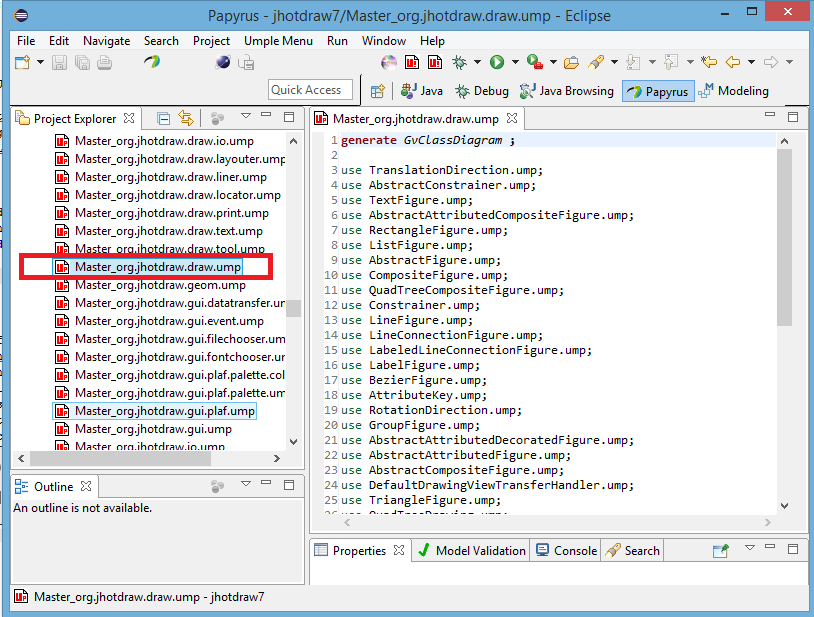
\includegraphics[width=0.80\textwidth]{Figures/jhotdrawMasterDraw.png} 
\caption{Master files used to compile JHotdraw}
\label{fig:jhotdrawMasterDraw}
\end{figure}

\newpage
\begin{sidewaysfigure}
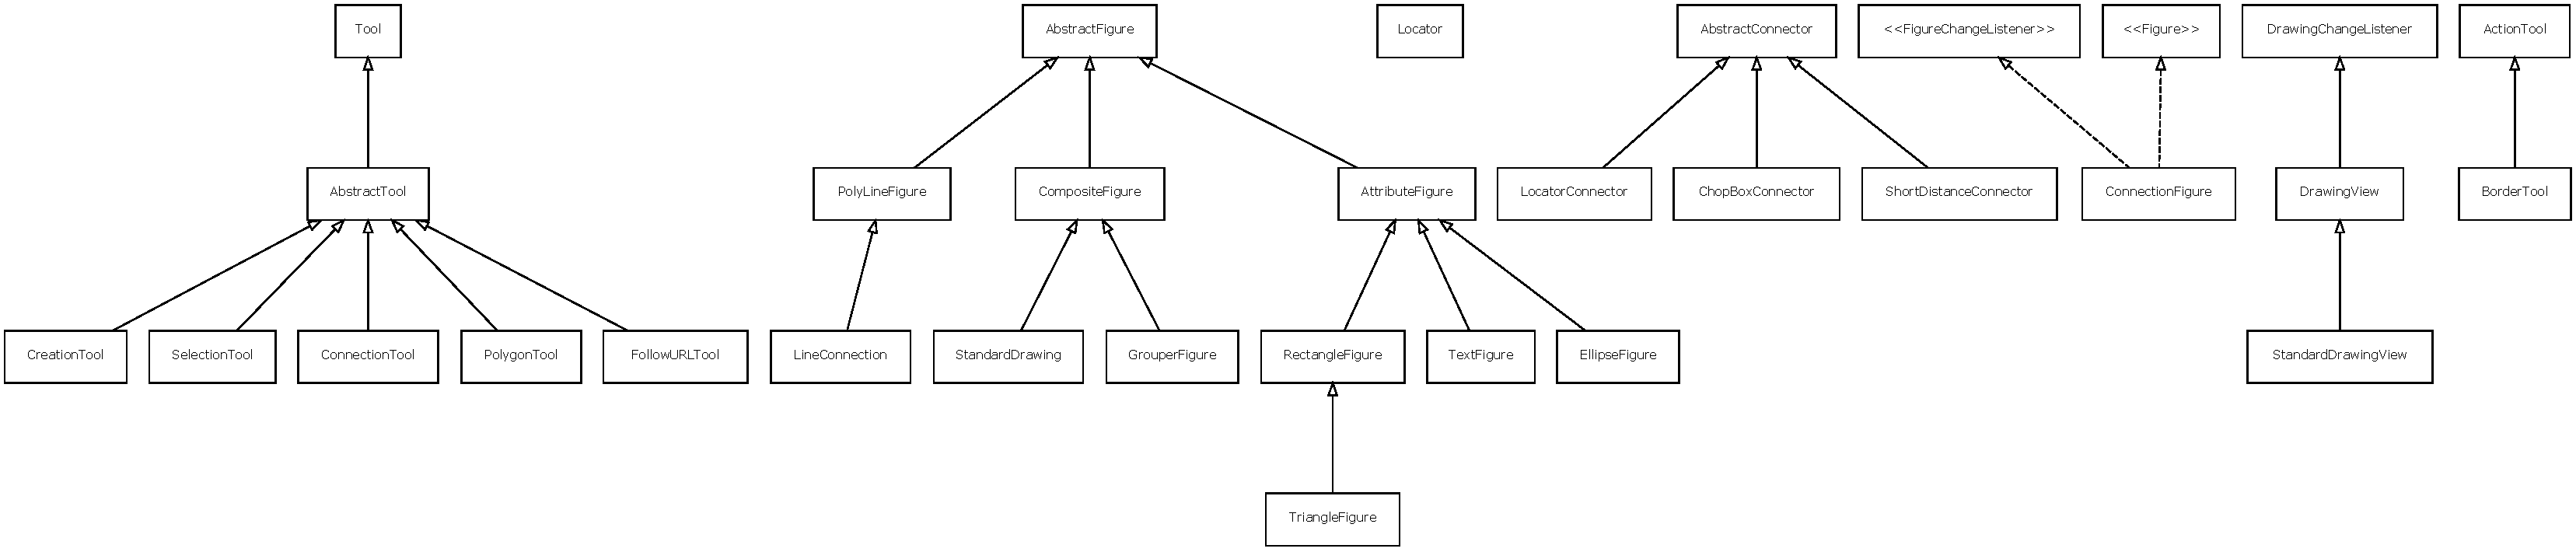
\includegraphics[width=0.99\textwidth]{Figures/jhotdrawuml.pdf} 
\caption{UML class diagram of package 'org.jhotdraw.draw' -  JHotdraw}
\label{fig:jhotdrawUMLClass}
\end{sidewaysfigure}

\subsection{Weka}
 
The next system we focused on was the machine learning tool Weka \cite{Weka}. As with our the first attempt at umplifying JHotDraw, our first attempt at automatically umplifying Weka resulted in the identification of the need for improvement to our rules; in particular some idioms it uses were not yet detected by our tool as it existed. For example, some classes in the classifiers package implement add() and remove() methods with different argument types. Also, the Confusion class declares add(RuleSet) and remove(Antecedent) to add and remove a set of rules from the evaluation algorithm. In addition, we detected, after execution of the test suite, that two classes were not compiling due to an unexpected constructor signature.

Another problem encountered while umplifying the Weka classes was related to inner classes. A Class such as \textit{weka.attributeSelection.BestFirst} uses two inner classes to manage the nodes and linked lists in a best-first search. The Umplificator was attempting to match types inside other data types, resulting in an infinite loop. In addition, since the Umple compiler does not currently support inner classes, the solution chosen to remedy this situation was to ignore inner classes and process them as Umple's `extra code'. 

Initial Umplification results for Weka nonetheless had a precision of 85\% when it comes to attributes and 38\% for 1-to-many associations. Table \ref{table:umplifiedResultsSystems1} summarizes the results. Note that a precision of 38\% doesn't mean that the Umplificator has missed 62\% associations of this type. It means that some of them were not correctly transformed into Umple (e.g. incorrect navigability, role names or transformation of accessor/mutator methods). The extensibility and flexibility of our tool allows us to add and refine rules without having to recompile the system. That is, rules in a external rule file (extension .drl) can be added to the working memory when running the Umplificator on the command line.

\subsection{Args4j - Modernization of the Code Base}

We reverse engineered Args4j \cite{UmpleFrameworkSANER15p494}, a small library that enhances the parsing of command line options and arguments in any Java application.

For every class in Args4j, our reverse engineering tool has produced two different files. The model design is expressed as an Umple model (i.e. Model.ump) and any algorithmic code is separated from the model (i.e. Model\_code.ump). Developers can now use the code generation technology to generate their system in any chosen programming language from the list of available languages in Umple.

If the modeler chooses to reproduce their system in the same language as it was before the reverse engineering process, we anticipate that the generated code will be of higher quality for a couple of reasons: First, we follow a rigorous test driven development approach in all of our framework components to ensure quality. Second, we have a state-of-the art code generator that respects associations multiplicity constraints and referential integrity \cite{UmpleAssociations}, and supports complex state machine code generation \cite{Badreddin2014EnhancedComposites}. Further details on the Umple API generated from various Umple constructs can be found at \cite{UmpleAPI}.

In another scenario, if the modeler chooses another programming language, as a target language, to generate the system, then they need to manually convert the algorithmic code in (files of type Model\_code.ump) to a new programming language such as C++. The distribution in terms of lines of code is as follows:

\begin{itemize}
\item Original Args4j Java source code is composed of 61 classes and 2223 lines of code.
\item Umplified Args4j source code is composed of 122 (2 per input class) umple files and 1980 lines of code in total.
\item Total number of lines of code in files containing modeling constructs (X.ump) is 312 LOC.
\item Total number lines of code in files with algorithmic/logic code (X\_code.ump) is 1668 LOC. If we exclude the umple class declarations and curly brackets, the number becomes 1424 LOC.
\end{itemize}

Consequently, to achieve the goal of translating Args4j into C++, a developer must translate 1518 lines of code (rather than 2223 lines of code). The benefits of umplification for the purposes of re-engineering may be more significant when processing larger software systems. This is marked as future work.


\section{Summary}

In this chapter, we have presented evaluation results showing that our approach and its current implementation are effective enough to be applied to real systems.

We have presented a multi-stage validation process evaluating the Umplificator from various perspectives
and ensuring the quality of the transformations as well as the systems umplified by our tool.

In the testing phase, we have presented an approach that independently tests the components of our tool. This is a generic approach that could be applied for the testing of programming languages, transformations technologies or compilers.

In the pre-validation phase, we have tested the umplification process using our own set of examples while in the initial phase of validation we have used 7 commercial open source systems. The results show that the precision and effectiveness of the tool improves when more and more systems are umplified, and any needed tuning is performed.

Finally, the second validation phase, validates the Umplificator with a set 100 randomly selected projects. At this point of time, seven open-source and commercial projects have been fully reverse-engineered successfully and 100 randomly selected systems were successfully umplified at level 1 (attributes ). 

% Got rid of efficiency above ... people will think the tool speeds up

It is our continuous objective to successively umplify more and more systems, with the hope that eventually our rule base will cover the vast majority of cases needed to successfully umplify new systems the Umplificator is presented with. However, even with a precision only in the high 80\% range (i.e. not yet at 100\%), our tool serves as a useful tool for umplification. Users can leave some variables un-umplified, or can manually umplify the rest.  
 % Evaluation

\lhead{\emph{\leftmark}}  
\chapter{Related Work}
\label{chap:related}
This chapter surveys previous work in reverse engineering approaches, and relates them to the work presented in this thesis. We will take a close look at studies that focused on generating UML models from source code written in object-oriented programming languages.
The following section describes the literature review methodology. We then present the results of our findings and a comparison between the different approaches and our own approach. 

\section{Literature Review Methodology}

This study has been undertaken as a literature review based on some of the guidelines proposed by Kitchenham \cite{kitchenham2004procedures}. Key parts of this systematic literature review are presented in this thesis.

\paragraph*{Research Question}

The main goal of this systematic review was to identify and classify different techniques for reverse engineering to UML. Specifically, we target the reverse engineering to UML of software systems by means of transformations. The high-level research question addressed by this study is:

\textit{What transformation techniques and/or methodologies for reverse engineering to UML can be identified from the literature?}

\paragraph*{Search process}

To search the databases, a set of strings was first created for each of the research questions based on keywords extracted from the research question, augmented with synonyms.

We designed a two-phase systematic review. In both phases, we searched for papers (including cited references) using the search engines in Table \ref{table:sourcesReviewed}. We then performed analyses of the related work to select a subset of papers that were truly relevant.

In the first phase we paid special attention to  existing surveys and literature review papers to ensure we found any literature review answering our research question.
In the second phase we  focused on technologies and techniques, as opposed to existing reviews. 

\begin{table}[ht]
\caption{Selected sources for the literature search}
\label{table:sourcesReviewed}
\centering
\begin{tabular}{ll}
\toprule
\rowcolor[HTML]{BBDAFF}
\textbf{Source}   & \textbf{Acronym} \\ 
\hline
IEEE Xplore	& IEEE   \\ 
ACM Digital Library &	ACM   \\ 
Springer Link	&SL   \\ 
Elsevier	&EV   \\ 
Scopus & SC   \\ 
Google Scholar &	GS   \\ 
Science Direct &	SD   \\ 
\hline
\end{tabular}
\end{table}

The sources for the search were chosen such that they included journals and conferences focusing on software engineering and program comprehension. 

The search resulted in an extensive list of potential papers. To ensure that all papers included in the review were related to the research questions, we defined detailed inclusion and exclusion criteria.  

\paragraph*{First Phase Queries and Results}

In the first phase of the review we used the following queries:
Related terms such as `design recovery' or `class diagram' `recovery' or `static' or `dynamic' were employed when some expected (already known/classified) papers did not appear as part of the results.

\begin{itemize}
\item `Reverse engineering' \textbf{AND}  UML \textbf{AND} `Survey'  4610 results
\item `Reverse engineering' \textbf{AND}  UML \textbf{AND} `systematic review' 210 results
\item `Reverse engineering' \textbf{AND}  UML \textbf{AND} `literature review' 669 results
\item `Reverse engineering' \textbf{AND}  UML \textbf{AND} `taxonomy' 22 results
\end{itemize}

By limiting the search to titles of articles, in the manner discussed below, we reduced the search results to a total of 33 papers. After manual inspection, only 5 papers were retained \cite{surveyMens},\cite{biehl2010literature}, \cite{DynamicSurvey}, \cite{Nelson1996} and \cite{Chikofsky}. 

The queries used in the second phase are enumerated below:

\paragraph*{Second Phase Queries}

\begin{itemize}
\item `Reverse engineering' \textbf{AND}  UML 
\item `Reverse engineering' \textbf{AND}  UML \textbf{AND} `class diagrams'
\item `Reverse engineering' \textbf{AND}  UML \textbf{AND}  `attributes'
\item `Reverse engineering' \textbf{AND}  UML \textbf{AND} `associations'
\end{itemize}

\paragraph*{Inclusion and exclusion criteria}

The databases searches resulted in an extensive list of potential papers. To ensure that all papers included in the review were clearly related and relevant to the research questions, detailed inclusion and exclusion criteria were defined. These criteria are summarized in Tables \ref{table:inclusionCriteria} - \ref{table:exclusionCriteria}. 
 The process followed for filtering the search result was:

\begin{enumerate}
\item Use the title to eliminate any papers clearly not related to the research

\item Use the abstract and keywords to exclude additional non-related papers

\item Read the remaining papers and eliminate those that do not fulfill the criterion in Table \ref{table:inclusionCriteria}.
\end{enumerate}

\begin{table}[ht]
\caption{Inclusion criteria}
\label{table:inclusionCriteria}
\centering
\begin{tabular}{l}
\toprule
\rowcolor[HTML]{BBDAFF}
\textbf{Inclusion criteria}    \\ \hline
  Papers that focus on software comprehension   \\\hline
  Papers that focus on software maintenance \\\hline
  Papers that focus on restructuring and re-engineering  \\\hline
  Papers describing model-to-model transformation techniques  \\\hline
  Papers describing model-to-text transformation techniques  \\\hline
\end{tabular}
\end{table}

\begin{table}[ht]
\caption{Exclusion criteria}
\label{table:exclusionCriteria}
\centering
\begin{tabular}{l}
\toprule
\rowcolor[HTML]{BBDAFF}
\textbf{Exclusion criteria}    \\ \hline
   Short-papers, tutorials, mini-tracks and workshop papers \\ \hline
   Studies whose results are not supported by any evidence or validated \\ \hline
\end{tabular}
\end{table}

\section{Results}

In the next section, we list and explain the criteria employed to assess the papers retrieved after filtering the results from the second-phase queries. Only 28 papers were retained from the originally 78 retrieved. The papers retained can mainly be categorized based on what type of technique they rely on: static or dynamic analysis of source code. Tables \ref{table:relatedPapers1} and \ref{table:relatedPapers2} list the 21 papers. The third column of the tables indicates if the approach uses dynamic analysis, static analysis or an hybrid approach (static + dynamic).

\begin{table}[h]
\caption{Filtered results from second-phase queries - Static approaches}
\label{table:relatedPapers1}
\centering
\begin{tabular}{p{6cm}|p{5cm}|p{3cm}}
\toprule
\rowcolor[HTML]{BBDAFF}
\textbf{Title}  & \textbf{Authors - Year - Ref} & \textbf{Category} \\ \midrule
1. Mining design patterns from C++ source code & Balanyi et al. - 2003 - \cite{Balanyi2003} &  Static (Graph-Based)
\\ \hline
2. Extraction and use of class dependency information for Java & Barowski et al. - 2002 \cite{Barowski} & Static 
\\ \hline
3. Recovering concepts from source code with automated concept identification & Carey et al. - 2007 - \cite{recoveringconcepts} &  Static
\\ \hline
4. A Patterns based reverse engineering approach for Java source code & Couto et al. - 2012 - \cite{Couto2012} & Static
\\ \hline
5. Recovering class diagrams from data-intensive legacy systems & Lucca et al.  - 2000 - \citep{Lucca2000}  &  Static
\\ \hline
6. Reverse engineering co-maintenance relationships using conceptual analysis of source code & Grant et al. - 2011 - \cite{grant2011reverse} & Static
\\ \hline
7. A systematic study of UML class diagram constituents for their abstract and precise recovery & Guéhéneuc - 2004 - \cite{GueheneucSystematic} & Static
\\ \hline
8. On reverse engineering an object-oriented code into UML class diagrams incorporating extensible mechanisms & Vinita et al. - 2008 - \cite{Vinita2008} & Static
\\ \hline 
9. Reverse-engineering 1-n associations from Java bytecode using alias analysis & Kang et al. - 2007 - \cite{Kang2007} & Static
\\ \hline
10. UML-based reverse engineering and model analysis approaches for software architecture maintenance & Riva et al. - 2004 - \cite{1357789} & Static
\\ \hline
11. Recovering UML class models from C++: A detailed explanation & Sutton et al. - 2007 -  \cite{Sutton2007} & Static
\\ \hline
12. Towards an AST-based approach to reverse engineering & Wang et al. - 2006 - \cite{4054609} & Static
\\ \bottomrule
\end{tabular}
\end{table}

\begin{table}[h]
\caption{Filtered results from second-phase queries - Dynamic and hybrid approaches}
\label{table:relatedPapers2}
\centering
\begin{tabular}{p{6cm}|p{5cm}|p{3cm}}
\toprule
\rowcolor[HTML]{BBDAFF}
\textbf{Title}  & \textbf{Authors - Year - Ref} & \textbf{Category} \\ \midrule
1. A simple static model for understanding the dynamic behavior of programs & Kelsen - 2004 - \cite{Kelsen2004} & Dynamic 
\\ \hline
2. Discovering Program's Behavioral Patterns by Inferring Graph-Grammars from Execution Traces &  Zhao et al. - 2008 - \cite{Zhao2008}& Dynamic (Traces)
\\ \hline
3. CPP2XMI: Reverse Engineering of UML Class, Sequence, and Activity Diagrams from C++ Source Code & Korshunova et al. - 2006 - \cite{cpp2xmi} & Hybrid
\\ \hline
4. Reverse engineering of design patterns from Java source code & Shi et al. - 2006 - \cite{4019568} & Dynamic
\\ \hline
5. Understanding applications through dynamic analysis & Antoniol et al. - 2004 - \cite{Penta2004Web} & Dynamic \\ \hline
6. Reverse engineering of object oriented code & Tonella et al. - 2005 - \cite{1553682} & Hybrid
 \\ \hline
7. A fully dynamic approach to the reverse engineering of UML sequence diagrams & Ziadi et al. -  2011 - \cite{5773385} & Dynamic
\\ \hline
8. Mining design patterns from existing projects using static and run-time analysis & Dobis et al. - 2011 - \cite{Huzar2011} & Hybrid
\\ \hline
9. Reverse-engineering of UML 2.0 sequence diagrams from execution traces & Delamare et al. - 2006 - \cite{Delamare06} &  Dynamic
\\ \bottomrule
\end{tabular}
\end{table}

In the next subsection, we present the most relevant (most cited and very related to our work) papers found. 
Although the results may convey that this area of research is mature enough, we believe there is still much work that can be done. The important fact is that the underlying research in this area makes us confident that our proposed approach contributes positively to the advancement of the reverse-engineering field.

\subsection{Most Relevant Papers}

A number of approaches have been presented in the literature for reverse engineering to discover associations and other related information from source code. Unlike our work, none of them is incremental or produces compilable artefacts. The majority of these produce in one single step a UML model derived from the source code \cite{Nelson1996}.

In \cite{Kollmann2001}, Gogolla and Kollman present a technique using both static and dynamic analysis to recover UML class models from C++ source code. This approach defines one of the few techniques for finding bidirectional associations.

In \cite{Barowski}, Barowski and Cross propose a technique to extract dependency information from Java bytecode. This approach, however, is not able to express correctly the multiplicity of the recovered associations.

Sutton and Maletic \cite{Sutton2007} propose a set of mappings that are intended to recover design-level UML class models from source code. They present their prototype tool, Pilfer, and use it to reverse engineer HypoDraw \cite{Hypodraw}, an open source tool.

%FINAL CHANGE START
%TLFINAL added space below to start paragraph; also added space at end of change and added the word a in one place

Gueheneuc \cite{GueheneucSystematic} presents a technique that infers associations, aggregation and composition relationships from Java programs using a constraint-based approach. 
The author formalized the class relationships at the implementation level as conjunctions of four different properties: Exclusivity, invocation-site, lifetime and multiplicity properties. 
However, their approach requires the availability and analysis of both static and dynamic models to build the class diagrams.
%FINAL CHANGE END

Commercial tools and widely used open source tools, including IBM Rational Software Architect \cite{ROSE}, Visual Paradigm \cite{VisualParadigm} and ArgoUML \cite{ArgoUML} lack configurability options and incremental reverse engineering capabilities. Moreover, they detect simple attributes, as well as one-way associations between classes but produce incomplete generated code (e.g. lacking methods and/or referential integrity) and fail to preserve semantics when the UML models derived from the tools are input in their own code generators \cite{kollmanToolsCurrent}. Some of the most popular reverse-engineering tools have been already discussed in Chapter \ref{chap:detections}.

Systa in her paper \cite{Systa} presented a tool named Fujaba \cite{Systa} that combines static analysis (graph matching) and dynamic analysis to detect pattern implementations in source code. This is so far the most popular and cited research tool relevant to this research found in the literature.

Bruneliere et al.\cite{ModiscoMain} introduced in their paper a model-driven reverse engineering tool, named Modisco, which has been developed as an Eclipse project and provides a set of generic tools to understand and transform complex models created out of existing systems. MoDisco uses JDT \cite{jdtProject} to discover Java elements in Java projects and allows the user to gather metrics and visualize results in a tree representation. Transformations can be performed on the discovered elements using another Eclipse technology, the ATL project \cite{jdtProject}, a model-to-model (M2M) transformation toolkit that we discussed earlier in this thesis.

TXL \cite{Cordy2006} is a rule-based language designed for a variety of source-to-source transformations tasks. We experimented with TXL as well as with ATL to implement  umplification, and, as described earlier, conclude that the two technologies were not ideal for incremental transformation of multi-language input models (Umple, Java, Umple+Java, etc.). A core concept behind umplification is that we want tool support for incrementality. We need to be able to load and transform a target model, already (partially) transformed by our tool so that users can convert Umple to Umple in steps of their choosing, always passing test cases, and maintaining confidence of the results. Existing model transformation tools proved not readily suitable for the multi-language incremental mode of use.

Paige et al. \cite{paigetowards} demonstrated the use of TXL in representing and for implementing efficient transformations between languages. A transformation from UML-to-Java were presented as part of their work. 

\subsection{Evaluation for Papers on Reverse-Engineering into UML}

 In this section, we list and define several important characteristics that we believe contribute to the comprehension of software systems. Our criteria emphasize the extraction of modeling constructs from source code.

The evaluation criteria we will use are as follows: 
\begin{itemize}

\item Scalability:  This refers to how well the solution works when the size of the system being studied increases.

\item Incrementality: This refers to the ability of the approach to be performed in incremental and small steps.

\item Validation:  Has the solution been validated by other software practitioners? Fully if so, Partial if it has been validated only by the authors. 

\item Usability: Is the tool easy to set up or use? N/A means that a tool is not available.

\item Target Programming Language: The programming language(s) that can be input into the tool.

\item Attributes Recovery: Is the approach/tool able to infer attributes from source code?

\item Associations Recovery: Is the approach/tool able to infer all different types of associations from source code? 
\end{itemize}

The outcomes of our evaluation can be:

\begin{itemize}
\item \textit{None} indicates that the criterion is not met or there is no evidence about this in the paper (or papers from the same author on the same topic).

\item \textit{Partial (P)} indicates that the criterion is partially satisfied.

\item \textit{Fully (F)} indicates that the criterion is fully satisfied and there is clear evidence of this.

\item \textit{N}  Not applicable. 
\end{itemize}

These criteria focus on how well the related studies solved the main topic of this thesis, i.e, reverse-engineering of object-oriented systems into UML. Note that the expected output from the techniques is UML and not Umple, as we are the first approach recovering Umple models from software systems.

Table \ref{table:finalResults} shows the above criteria applied to the key papers. 

\begin{table}[ht]
\caption{Application of the evaluation criteria to the key papers}
\label{table:finalResults}
\centering
\begin{tabularx}{\textwidth}{X|lllllll}
\toprule
\rowcolor[HTML]{BBDAFF}
\textbf{Authors-Year-Ref}  & \rotatebox{90}{\textbf{Scalability}} & \rotatebox{90}{\textbf{Incrementality}}& \rotatebox{90}{\textbf{Validation}}& \rotatebox{90}{\textbf{Usability}}& \rotatebox{90}{\textbf{Target Prog. Lang.}} & \rotatebox{90}{\textbf{Attribute Recovery}}& \rotatebox{90}{\textbf{Associations Recovery}} \\ \hline
Barowski et al. - 2002 \cite{Barowski} & N & N & P & N & Java  & P & P \\ \hline
Grant et al. - 2011 - \cite{grant2011reverse} & P  & N & P &  F & Java  & F & P \\ \hline
Gueeheneuc - 2004 - \cite{GueheneucSystematic} & P & P& F  & F &Java  & F & F \\ \hline
Vinita et al. - 2008 - \cite{Vinita2008} & N & N & N & N & Cpp & P & P \\ \hline
Kang et al. - 2007 - \cite{Kang2007} & N & N& N & F &Java & F & P \\ \hline
Sutton et al. - 2007 -  \cite{Sutton2007} & N & N & P & F & Cpp & P & P\\ \hline
Korshunova et al. - 2006 - \cite{cpp2xmi} & P & N & P & F & Cpp & F & P\\ \hline
{Umplification} & \textbf{P} & \textbf{F} & \textbf{P}  & \textbf{F} & \textbf{Java,Cpp} & \textbf{F} & \textbf{P} \\ 
\hline
\end{tabularx}
\end{table}

What mainly differentiates our work from other work is incremental refactoring, the configurability of the mappings rules, the form of the output (model and code as a single entity), and the preservation of semantics when code is generated from the recovered models.

As the last row of the  table indicates, our approach performs well for most of the covered criteria. However, one of the most important characteristics of our approach is that it can be easily extended to cover those missed parts. % Related Work

\lhead{\emph{\leftmark}}  % Set the left side page header to 
\chapter{Conclusions and Contributions}
\label{chap:conclusion}
In this thesis we presented a reverse engineering approach called umplification and the corresponding tool, the Umplificator. Umplification is the process of transforming step-by-step a base language program to an Umple program that merges textual modeling constructs directly into source code. 

\section{Summary of Answers to Research Questions}

We outline how the umplification approach and its underlying implementation addresses the  research questions identified at the beginning of the thesis.

\paragraph*{RQ1. To what extent can we achieve automated umplification?}

In Chapter \ref{chap:technology} we addressed this research question by exploring technology alternatives and developing a tool to implement the umplification reverse engineering capabilities. The effectiveness of the transformations were then evaluated in Chapter \ref{chap:evaluation}. The evaluation results showed that our approach and its current implementation are effective and efficient enough to be applied to real systems. In particular we were able to successfully umplify many real open-source systems at varying degrees of effectiveness, and were able to iteratively improve this effectiveness by adjusting rules.
 
\paragraph*{RQ2. What transformation technology and transformations  will work effectively for umplification?}

In Chapter \ref{chap:technology}  we discussed our experiments with ATL and TXL approaches. However in the end we selected an approach that uses a) the mature xDT family of parsing libraries (JDT, CDT, etc.) to process both code and textual models, and build in memory models; b) the Drools tool to transform the in-memory models, accomplishing the core umplification task; and c) our own generator technology to produce revised versions of the system. Details of the approach are expanded in the answer to the next research question.

\paragraph*{RQ3. What should be the architecture, design and implementation of an umplification tool?}

The implementation of the Umplificator, combining the technologies mentioned above, was discussed in depth in Chapter \ref{chap:technology}. The advantages of the selected approach enabled the following aspects, each of which we discussed in Chapter \ref{chap:technology}.

\begin{enumerate}

\item Separation of concerns

\item Speed and scalability

\item Centralization of knowledge

\item Multi-level testing

\item Robust parsing 

\item Efficiency

\item Agile development 

\item Extensibility

\item Reusability

\end{enumerate}

\paragraph*{RQ4. What would be an effective process for improving the accuracy of the umplification tool?}

We presented in Chapter \ref{chap:evaluation} an approach adapted from the model often used in machine learning that  considerably improved the precision and recall of our transformations. This validation approach takes one set of systems as the `training set' and then takes another set as the `testing set' to see how well the Umplificator performs on unknown systems. The process is iterative; in other words, we tune the system based on problems found when working with the testing set. 
One type of problem is  failure of the umplification to complete, at its various levels. Another type of problem is automatic umplification that does not match manual umplification of one of the test systems. To solve these problems, the Umplificator can be readily tuned by adding new mapping rules to cover `False Negative' cases, by refining existing rules to cover `False positive' cases or by correcting the refactoring helper functions when code injections are incorrectly inserted.

\section{Contributions}

The main contributions of this thesis are as follows:

% FINAL CHANGE START - NOT DONE YET
\begin{enumerate}
\item The overall concept of umplification and the defined levels of refactoring;

\item An understanding of how umplification compares with other reverse-engineering techniques (incrementality, minimal adjustment of code to prevent disruption);

\item The implementation and analysis of integrating different transformation technologies;  resulting in the Umplificator tool itself;

\item Case studies of Umplification, demonstrating strengths, weaknesses and opportunities. Results presented in this thesis are reproducible and repeatable. Popular and highly cited open-source projects such as JHotdraw and Weka are now fully rewritten in Umple. We also made improvements to Umple compiler  to support abstract classes, interfaces and top-level enumerations, as needed to support the case studies.

\item Mapping rules for Umplification and the language for expressing these. We have employed a popular rule management system known as Drools. Drools offers a native rule language with a simple Java-like syntax. Rules can easily be added and refined by means of an editor with syntax highlighting and code completion.

\item Detection of associations in a body of source code written in an object-oriented;
programming language. We have investigated how associations are employed in both forward and reverse engineering and proposed a set of heuristics for the detection of these in source code.
\end{enumerate}
% FINAL CHANGE END
Major advantages of our work, as compared to other reverse engineering approaches, are the concept of incrementally, the ease of addition of mapping rules, and the preservation of the system in a textual format.

\section{Future Work}

Although the results presented here have demonstrated the effectiveness of the umplification approach, it could be further developed in a number of ways:

\begin{description}
\item[Umplify more Projects] We plan to apply the approach to other open source systems, gradually increasing the ability of the Umplificator to obtain a higher and higher first-pass precision on new systems it encounters.
% FINAL CHANGE START
\item[Incorporate other object-oriented programming languages] We plan to add support for C++ and PHP languages. In particular, we need to create new mapping rules for those idioms that were not already considered for Java. For instance, in C++ we need to analyze the content of header files. The work to be done targets exclusively the \textit{Transformer} component of the Umplificator, since parsing and base language model generation is achieved by means of the CDT/PDT frameworks.
% FINAL CHANGE END
\item[State Machines Support] We also plan integrate the mapping rules for state machines and refine some of the existing rules to make them more maintainable. Our team's decision to consider state machines as the next model construct to analyze is based on the observation that there seems to be interesting research opportunities in that area.

\item[IDE Integration] It would be beneficial to improve tools to support better IDE integration including a step-by-step guide to indicate the level of umplification achieved of a software project. The Umplificator Eclipse plugin could be improved by adding an Eclipse perspective to better present the available features of the Umplificator to end-users.

\item[Evaluation with real developers] To date, we have theoretically demonstrated the benefits of the approach, as well as demonstrated its industrial practicality by  reverse-engineering open-source systems with the tool.  A next logical step, outside the scope of this thesis, is to evaluate its efficiency and precision with a representative set of software practitioners.  In particular,  it would be beneficial to subject the Umplificator to evaluation with real developers The process might work as follows: 1) Arrange for a group of users to umplify some small systems, some by hand, and others with the Umplificator. 2) Measure the speed and correctness of the result, and also administer a questionnaire to the participants. 3) Video developers as they umplify larger programs, while  encouraging them to think aloud. 4) Analyze the videos looking for places where the participants make mistakes, express frustration, spend a lot of time thinking, have to refer to help, etc. 5) Evaluate in a similar manner the language used to express the mapping rules. 

\item[Exploring other types of software] Investigating the integration of algorithms for the umplification of mobile and Web applications which require enhancing the Umple Language itself and our tool support.

\item[Umplifying code that matches other model elements] Investigating the detection of additional software patterns aligning with those supported by Umple (e.g keys) is also an interesting research opportunity for future researchers.

\end{description} % Conclusions and Contributions

%% ----------------------------------------------------------------
% Now begin the Appendices, including them as separate files

\addtocontents{toc}{\vspace{2em}} % Add a gap in the Contents, for aesthetics
 
%\appendix % Cue to tell LaTeX that the following 'chapters' are Appendices

%\input{Appendices/AppendixA}	% Appendix Title

%\input{Appendices/AppendixB} % Appendix Title

%\input{Appendices/AppendixC} % Appendix Title

\addtocontents{toc}{\vspace{2em}}  % Add a gap in the Contents, for aesthetics
\backmatter

%% ----------------------------------------------------------------
\label{Bibliography}
\lhead{\emph{Bibliography}}  % Change the left side page header to "Bibliography"
\bibliographystyle{unsrtnat}  % Use the "unsrtnat" BibTeX style for formatting the Bibliography
\bibliography{Bibliography}  % The references (bibliography) information are stored in the file named "Bibliography.bib"

\end{document}  % The End
%% ----------------------------------------------------------------